%% IFBThesis Latex Template Version 1.0, a fork of :
%% 	RiSE Latex Template - version 0.5
%%
%% IFBthesis latex template for thesis and dissertations
%% https://github.com/auyer/IFBtcc
%%
%% (c) 2017 Rafael de Campos Passos (rcpassos@ieee.org)
%%
%% This document was initially based on RiSE Latex template, from Yguaratã
%% Cerqueira Cavalcanti
%%
%% GENERAL INSTRUCTIONS
%%
%% We strongly recommend you to compile your documents using pdflatex command.
%% It is also recommend use the texlipse plugin for Eclipse to edit your documents.
%%
%% Options for \documentclass command:
%%         * Idiom
%%           pt   - Portguese (default)
%%           en   - English
%%
%%         * Text type
%%           bsc  - B.Sc. Thesis
%%           msc  - M.Sc. Thesis (default)
%%           qual - PHD qualification (not tested yet)
%%           prop - PHD proposal (not tested yet)
%%           phd  - PHD thesis
%%
%%         * Media
%%           scr  - to eletronic version (PDF) / see the users guide
%%
%%         * Pagination
%%           oneside - unique face press
%%           twoside - two faces press
%%
%%		   * Line spacing
%%           singlespacing  - the same as using \linespread{1}
%%           onehalfspacing - the same as using \linespread{1.3}
%%           doublespacing  - the same as using \linespread{1.6}
%%
%% Reference commands. Use the following commands to make references in your
%% text:
%%          \figref  -- for Figure reference
%%          \tabref  -- for Table reference
%%          \eqnref  -- for equation reference
%%          \chapref -- for chapter reference
%%          \secref  -- for section reference
%%          \appref  -- for appendix reference
%%          \axiref  -- for axiom reference
%%          \conjref -- for conjecture reference
%%          \defref  -- for definition reference
%%          \lemref  -- for lemma reference
%%          \theoref -- for theorem reference
%%          \corref  -- for corollary reference
%%          \propref -- for proprosition reference
%%          \pgref   -- for page reference
%%
%%          Example: See \chapref{chap:introduction}. It will produce
%%                   'See Chapter 1', in case of English language.
%%
%% Citation commands:
%%          \citet (from natbib) -- To cite a reference as part of the narrative
%%          \citep (from natbib) -- To cite a reference between parenthesis
%%          citationblock environment -- To produce direct citation blocks according to the ABNT

\documentclass[pt,oneside,onehalfspacing,bsc]{ifbthesis}

\usepackage{colortbl}
\usepackage{color}
\usepackage[table]{xcolor}
\usepackage{microtype}
\usepackage{bibentry}
\usepackage{subfigure}
\usepackage{multirow}
\usepackage{rotating}
\usepackage{booktabs}
\usepackage{pdfpages}
% \usepackage{caption}
\usepackage{lipsum}
\usepackage{sectsty}
\usepackage{float}
\usepackage{pdfpages}
\usepackage{longtable}
\usepackage{tabularx}
\usepackage{natbib}

%% Set the language used in your code in the block above

% \captionsetup[table]{position=top,justification=centering,width=.85\textwidth,labelfont=bf,font=footnotesize}
% \captionsetup[lstlisting]{position=top,justification=centering,width=.85\textwidth,labelfont=bf,font=footnotesize}
% \captionsetup[figure]{position=bottom,justification=centering,width=.85\textwidth,labelfont=bf,font=footnotesize}

%% Chapter and (Sub)Section fonts must be same size as text (12)
\sectionfont{\fontsize{12}{15}\selectfont}
\subsectionfont{\fontsize{12}{15}\selectfont}
\subsubsectionfont{\fontsize{12}{15}\selectfont}

%% Change the following pdf author attribute name to your name.
\usepackage[linkcolor=black,
            citecolor=black,
            urlcolor=black,
            colorlinks,
            pdfpagelabels,
            pdftitle={Rise Thesis Template (ABNT)},
            pdfauthor={Rise Thesis Template (ABNT)},
            breaklinks=true]{hyperref}

\address{BRASÍLIA}

\universitypt{Instituto Federal de Brasília}
\universityen{Federal Institute of Brasilia}

\campus{Campus Taguatinga}

\departmentpt{Departamento de Computação}
\departmenten{Computer Department}

\programpt{Bacharelado em Ciência da Computação}
\programen{Bachelors in Computer Science}

\majorfieldpt{Ciência da Computação}
\majorfielden{Computer Science}

\title{Melhoria do Sistema Integrado de Divulgação de Informações do IFB: aperfeiçoamento da integração ao Facebook e aplicativo móvel}

\date{2018}

\author{Maxwell Borges Bezerra}
\adviser{Prof. Me. Daniel Saad Nogueira Nunes}
%\coadviser{Nome dompleto do co-orientador }

% Macros (defines your own macros here, if needed)
\def\x{\checkmark}
%\let\lstlistoflistings\origlstoflistings
\begin{document}

\frontmatter

\frontpage

\presentationpage

\begin{fichacatalografica}
% 	\FakeFichaCatalografica % Comment this line when you have the correct file
    %\includepdf{documentacoa/ficha} % Uncomment this
    \includepdf[pages=-]{documentacao/ficha.pdf}
\end{fichacatalografica}

\banca

\begin{dedicatory}
    Dedico essa obra aos meus amigos e ao orientador, estes que me apoiaram, me zoaram e passaram raiva durante todo o desenvolvimento, são eles: Leandro Chaves, Evio Fragoso, Mauricio Arruda, Flavia Dias e Daniel Saad.
\end{dedicatory}

\acknowledgements
Agradeço a minha família por me apoiar em todas as minhas decisões, até mesmo nos momentos mais difíceis, aos meus amigos da faculdade, por todos os momentos que tivemos e a cumplicidade dos mesmos. Mas não somente, agradeço a todos que de alguma forma participaram da minha vida e me proporcionaram momentos e aprendizagens que me fizeram uma pessoa melhor. Deixo meus sinceros agradecimentos ao meu orientador Daniel Saad Nogueira Nunes por me instruir durante todo o desenvolvimento do trabalho.

\gdef\resumoname{Resumo} 
{\parindent0pt
	\begin{resumo}
Este trabalho apresenta o Sistema Integrado de Divulgação de Informações do IFB Câmpus Taguatinga - SID que, por meio de uso dos conceitos de sinalização digital e marketing digital, visa veicular notícias em forma de publicações que são repassadas por meio de televisões no ambiente do \textit{Campus} ou fora dele por meio de um aplicativo móvel instalado nos celulares. 

Foram realizadas diversas alterações no sistema inicial chamado de SIDv2. As alterações vão desde modificações na arquitetura existente para implementação de novas funcionalidades, até a implementação de um aplicativo exclusivos para celulares. As alterações foram realizadas de modo a flexibilizar a implantação de novas funcionalidade e serviços, para que outros sistemas pudessem fazer de um mesmo sistema. 

O SIDv3 também passou a possuir a integração completa com a rede social Facebook, disponibilizando a possibilidade de realização de publicações em páginas do Facebook e apresentação dos conteúdos referentes a essas publicações. Com isto é realizado uma junção de meios que anteriormente eram distintos no IFB.

Além disso, o aplicativo \textit{mobile} servirá de forma a repassar as divulgações criadas, além de realizar o consumo de uma API fictícia para interação entre alunos e professores com a troca de mensagens. Esse consumo de API possibilita uma futura integração com o Sistema de Gestão Acadêmica - SGA.
    
 \noindent
 %\textbf{Palavras-chaves}: latex. abntex. editoração de texto.
\end{resumo}

}

\abstract
% Write your abstract in a file called abstract.tex
{\parindent0pt
	\begin{resumo}[Abstract]
 \begin{otherlanguage*}{english}
   This is the english abstract.

   \vspace{\onelineskip}
 
   \noindent 
   \textbf{Key-words}: latex. abntex. text editoration.
 \end{otherlanguage*}
\end{resumo}

}

% List of figures
\listoffigures

% List of Codes
\lstlistoflistings

% List of tables
\listoftables

% List of acronyms
% Acronyms manual: http://linorg.usp.br/CTAN/macros/latex/contrib/acronym/acronym.pdf

% Summary (tables of contents)
\tableofcontents

\mainmatter

\chapter[Introdução]{Introdução}
Apesar de muito usada, a definição exata de mídia é complicada de ser explicada. De acordo com \cite[p.49]{guazina2007}, o uso predominante do termo ``mídia'' é para representar um conjunto de meios de comunicação, representado por meios de comunicação em massa como jornais, televisão, rádio, cinema e \textit{Internet}.

Sendo a mídia, talvez, responsável por introduzir mudanças comportamentais e comerciais nas mais diferentes sociedades, seja ela por informações presentes em canais de televisão, outdoors ou até mesmo panfletos, em ambientes públicos ou privados, \cite[p.3]{escobar2007} propõe que a mídia é capaz de redefinir ``o modo como o homem se comunica e se relaciona com os semelhante.''

Para se ter uma ideia do poder que a mídia tem, para \cite{silva2007}, quando a população não tem acesso a outras fontes de informações, as notícias e mensagens veiculadas pelas mídias são muitas vezes vistas como verdades inquestionáveis. \cite[p.53]{guazina2007} aponta que os meios de comunicação são visto como potenciais construtores de conhecimento e formadores de compreensão sobre mundo e política.

Ainda sobre a influência da mídia, para \cite[p.54]{hjarvard2012}, surge o conceito de midiatização. Para ele, a midiatização é um termo usado para caracterizar a influência da mídia e coloca também a midiatização como ``um processo contínuo em que os meios alteram as relações e o comportamento humanos e, assim, alteram a sociedade e a cultura''. 

Com o passar dos anos, a mídia foi obtendo novas formas, as divulgações de forma estática e mais tradicionais (revistas, jornais e canis de televisão) foram deixando de serem os meios mais eficientes de se expor um conteúdo ou propaganda, para \cite{meditsch2001} o advento da \textit{Internet} e sua popularização trouxe uma ameaça para estes meios, então foi necessário que novas formas de expor conteúdos fossem pensadas e desenvolvidas em conjunto com essa nova ferramenta.

Nos meios de comunicação em massa sempre estão presentes os mais diversos tipos de propagandas e divulgações, o \textit{marketing} é responsável por criar e melhorar as ferramentas que tem como objetivo influenciar pessoas a adquirir ou aderir determinado produto ou serviço. Assim como a mídia, novas formas e ferramentas de \textit{marketing} também foram surgindo, ampliando os meios de como as informações são repassadas. 

Para a ampliação, foi necessário que os caminhos da publicidade e da tecnologia fossem se convergindo para se então definir um novo conceito de \textit{marketing}, o \textit{marketing} digital. O \textit{marketing} digital conta com novas tecnologias de comunicação que para \cite[p.2]{escobar2007}, isso coloca a interatividade em evidencia, então, a utilização de novas ferramentas mais interativas com seu receptor, tornam a leitura menos monótona e passível de atingir uma maior atenção do espectador de forma mais consistente.  

As vantagens para a utilização da interatividade estão presentes em diversas formas, como por exemplo para \cite[p.4]{escobar2007}, transmissões ao vivo por rádio ou televisão permite o acesso a um dado acontecimento no exato momento em que ele acontece, mas quando se tem o advento da Internet coloca-se a possibilidade de interação com a informação que é recebida, isso quase que instantaneamente, onde os integrantes atuam simultaneamente, comentando ou opinando sobre aquele determinado assunto. Para \cite{deuze2002}, o advento da \textit{Internet} traz a possibilidade do público ``responder, interagir ou mesmo customizar certas histórias''. 

A evolução do \textit{marketing} digital trouxe consigo a união das mídias sociais e dispositivos móveis. Isso permite não somente que as informações circulem fora de ambientes específicos, mas também que os receptores das informações transmitidas possam interagir quase que em tempo real com o conteúdo que é apresentado. Para \cite{santos2014}, no contexto do novo cenário da web é necessário um marketing em ambiente digital.

Para \cite[p.7]{machado2010}, o rápido crescimento das organizações juntamente com a Internet as obrigou a aderirem novos conceitos de gestão e apresentação das informações, usando não somente os veículos de comunicação e as mídias digitais. Pensando na maior abrangência, surge o conceito de sinalização digital, que para \cite[p.37]{machado2010}, consiste na transmissão de conteúdo via Internet, onde essa mesma informação pode se ter receptores no mais diversos locais, independente de cidade, estado ou país com o uso de painéis e televisores apresentando informações e propagandas de forma dinâmica, nos mais diversos pontos e com a possibilidade de gerenciá-las remotamente de acordo com a necessidade. 

As mídias sociais também possuem seu importante papel para disseminação de uma informação ou conteúdo e vem se tornando uma das ferramentas mais atraentes para divulgações, para \cite{rosa2010} isso se deu pelo seu grande uso e por elas se tornarem a extensão da vida real. Não apenas por ser um dos meios mais acessados atualmente, mas também por conta da maior facilidade de interações dos espectadores, usuários e empresas que para \cite{rosa2010} esse tipo de mídia permite as empresas encontrarem a melhor solução para seus objetivos. 

Com o passar dos anos os dispositivos móveis estão sendo cada vez mais usados pelas pessoas, isso vem atraindo cada vez mais o foco dele como ferramenta para divulgação de informações. A pesquisa da \cite{fgv2017} aponta que até outubro de 2017 teria-se 208 milhões de aparelhos ativos no brasil e que até maio de 2018 terá cerca de 220 milhões de \textit{smartphones} ativos, mais de 1 aparelho por habitante. 

Não somente pelo grande número de dispositivos, mas também pela grande integração com as redes sociais que segundo a \cite{forbes2016}, pesquisas feitas pela agencia eMarketer afirmavam que até o final de 2016, 42\% da população da América latina iriam acessar regularmente as redes sociais, em 2016 estimava-se que 74\% da população do Brasil que usasse a internet no pais teriam uma conta no Facebook, se comparado o mundo todo, o número chega a 2 bilhões de usuários em 2017. 

O Campus, para divulgação de notícias e as mais variadas informações, se utiliza principalmente da sua página oficial e sua página oficial no Facebook. Para utilização desses meios, é necessário que os administradores façam publicações independentes para cada uma das páginas, onerando o trabalho do mesmo, além disso, as páginas não são bem divulgadas, muitas vezes os estudantes e visitantes nem ficam sabendo das notícias que lá são publicadas. Além disso, os professores contam com poucas formas fáceis e intuitivas para repassar informações a seus alunos.

Essa falta de integração entre os veículos institucionais, que atuam de forma independente acabam degradando a qualidade e a disseminação da notícia, não somente pela falta de um sistema integrado mas também pela complicada interação e acesso dos usuários com as atuais mídias, o que acaba afetando o interesse de acompanha-la.

O Sistema Integrado de Divulgação de Informações do IFB (SID) oferece uma maior visibilidade das notícias, sendo possível por meio painéis espalhados pelo campus, uma melhor interação da comunidade com as notícias, apresentando nos painéis os comentários que foram publicados nas mídias sociais, além de uma melhor forma de comunicação entre professor e aluno, oferecendo um aplicativo \textit{mobile} que simula o Sistema de Gestão Acadêmica (SGA) em conjunto com a apresentação das notícias.

\section{Motivação}
A atenção do espectador a uma determinada informação que está sendo apresentada é algo crucial para o sucesso das notícias que estão sendo exibidas, quanto melhor disseminada ela for, maior a chance de sucesso. Quando se tem uma interatividade com o telespectador a sua atenção é atraída. Nesse intuito, a interatividade e o dinamismo com a utilização de ferramentas atuais, usadas no dia a dia, é algo que pode atrair a atenção do usuário, fazendo-o ter interesse em acompanhar e participar de uma determinada noticia ou matéria, tornando-a mais facilmente acessível. 

Atualmente, o IFB utiliza o seu perfil do Facebook e sua página oficial como principal forma de veiculação das notícias referentes a informações da instituição, sejam elas notícias de eventos ou institucionais. Para realizar a criação de uma nova notícia é necessário o administrador acessar cada página e realizar uma postagem independente em cada uma delas. 

Então se tem a necessidade de melhor exposição das notícias, de uma forma de contato fácil e rápida com a comunidade acadêmica, de um sistema mais interativo, com suporte a gestão academia e com uma forma simplificada de contato entre professor e aluno. Pensando nisso, vê-se a necessidade de um sistema onde é possível expor notícias referentes a instituição com facilidade, contando com uma melhor facilidade de acesso e interatividade do espectador dessa notícia, por meio de comentários na publicação e apresentação em tempo real.

Além disso, a comunicação entre professor e turma é feita geralmente por meio físico, e-mail ou necessitando de outros \textit{softwares} complementares, sendo necessário o professor ter e-mails individuais de cada aluno ou de turma para encaminhar qualquer notícia e isso acaba sendo ruim tanto para os professores, quanto para os alunos. 

\section{Proposta}
Com uso da estrutura cliente-servidor e tendo o sistema SID em sua versão 2 implementado por \cite{sobrinho2017} como base, é proposto a elaboração da terceira versão. Com o uso dos conceito de sinalização digital e marketing digital, a proposta é fazer com que o sistema apresente conteúdos referentes ao IFB e essas informações tenham integração com o Facebook, apresentando postagens e comentários devidamente moderados em tempo real nas telas espalhadas por locais de maior movimento do Câmpus Taguatinga do Instituto Federal de Brasília ou nos dispositivos móveis de cada pessoa. 

O sistema proposto, visa proporcionar a integração dos meios usados atualmente para apresentação das informações referentes ao Câmpus, além da inclusão de outros meios. A sistema fará a integração entre a página do Facebook da instituição, painéis de notícias e dispositivos móveis dos alunos ou professores.

Portanto, a ideia do SID, é prover a melhor interatividade do espectador com as publicações acadêmicas e o administrador ter uma maior facilidade de criação e edição das publicações vinculadas as redes sociais, integrando vários serviços em um único.

Na versão para dispositivos móveis, além da apresentação das notícias, os professores e os alunos terão acesso a uma nova funcionalidade, o docente poderá enviar informações e avisos distintos para cada aluno ou turma, enquanto os alunos poderão acessar a cada mensagem enviada pelo professor para a turma em que ele está cadastrado, através de um login usando uma matricula e senha fictícia cadastrado no bancos de dados que simula plataformas acadêmicas já existentes, não sendo possível ainda o uso de dados reais por restrições de acesso as essas plataformas.

\section{Objetivos}
\subsection{Objetivos Gerais}
Com objetivo de uma melhor e fácil disseminação das informações e propagandas pertinentes ao IFB - Câmpus Taguatinga, o sistema deverá ser capaz de proporcionar objetividade e simplicidade nas informações a serem repassadas. Além de painéis instalados pelo Câmpus, ele deve ter a integração com as mídias sociais como o Facebook, unificando os atuais sistemas de comunicação do IFB.

Além das otimizações necessárias no sistema, é feito uma filtragem de comentários antes da exibição no sistema, esse filtro de comentários servirá para que não sejam apresentados comentários abusivos e que se tenha comentários mais propícios a reações positivas por partes dos telespectadores.

Com a versão mobile do sistema, o aluno poderá não só ter acesso as informações que serão publicadas de forma geral para o Câmpus, mas também aos conteúdos específicos através de uma matricula fictícia do aluno ou professor que simula o sistema usado pelo IFB, no caso o SGA. 

O aplicativo \textit{mobile} contará com três telas, a primeira é para exibição das publicações, a segunda tela servirá para que o professor possa encaminhar mensagens para uma turma em que ele leciona ou para um aluno especifico, a terceira tela é a do aluno, onde ele poderá verificar todas as mensagens que a turma em que ele está matriculado possui.

\subsection{Objetivos Específicos}
\maxwell{ARRUMAR OS OBJETIVOS - comentários 105 a 111}

	 \begin{itemize}
	\item Implementar um sistema para um âmbito mais acadêmico, para melhorar a disseminação de informações dentro do Câmpus.
	 	
	\item Melhorias do sistema usado como base, o SID \cite{sobrinho2017}.
	
	\item Aprimorar o uso da ferramenta Graph API para uma melhor integração do sistema com o Facebook, recuperando mensagens, curtidas entre outras informações que venham a ser necessárias.
	
	\item Integrar o sistema com outras mídias sociais.
	
	\item Implementação de uma versão mobile do sistema, para possíveis consultas ou exibição do conteúdo, tornando a exibição das informações multiplataforma, exibindo-a em painéis, TVs, páginas de Internet ou celulares.
	
	\item  Implementar um sistema em que os docentes possam trocar mensagens com alunos das turmas em que ele leciona.
	\end{itemize}
\section{Metodologia}
A revisão de bibliografia é usada como meio de direcionamento do trabalho, usando comparações entre ferramentas desenvolvidas com o proposito principais de sinalização e \textit{marketing} digital, partindo de tais soluções com o objetivo de avaliar os pontos negativos tendo como base as necessidades do Câmpus e então juntar ao processo de desenvolvimento os elementos que forem selecionados como principais e que são responsáveis por efetivar a disseminação da informação ao sistema de forma descentralizada e com o auxílio de ferramentas utilizadas no contexto WEB.
	 
Usando o SID versão 2 como sistema base, uma estrutura cliente-servidor e conexão a \textit{Internet} , será implementado no sistema as interações com as redes sociais. As informações serão apresentadas em multiplataforma que podem ser televisores, painéis, páginas web ou celulares, essas informações podem ser alteradas acessando ao servidor com o sistema instalado e conectado a Internet. Após serem criadas ou modificadas, as publicadas poderão ser transmitidas e acessadas pelos clientes em distintas plataformas ao mesmo tempo.

A metodologia presente neste trabalho está direcionada aos aspectos específicos do desenvolvimento de ferramentas computacionais com o intuito de melhoria no processo de comunicação e veiculação de informações através de várias plataformas, sejam elas \textit{mobile}, WEB ou painéis. Para a versão \textit{mobile} do sistema, será usado um \textit{framework} de desenvolvimento específica para a plataforma. 

\maxwell{FALAR SOBRE METODOLOGIAS - comentários 131 a 134}

\section{Organização}

\chapter[Trabalhos Relacionados]{Trabalhos Relacionados}
\section{OOZO}
Atualmente, uma solução encontrada na literatura que faz integração entre \textit{marketing} digital e o conceito de sinalização digital é o software \cite{oozo2017}, com suporte a multiplataformas como Linux, Windows, MacOs, Raspberry e pagina WEB, suas publicações podem ser exibidas online como \textit{streaming} ou também em telas públicas que são painéis colocada em locais estratégicos de grande acesso público e com programações especificas, designadas pelo desenvolvedor com a assinatura de um serviço de exibição.

Na pagina de login do aplicativo é possível criar uma nova conta, usar uma conta do Facebook ou Google. Na sua versão profissional, a mais completa, é possível sincronizar redes sociais, capturar comentários com \textit{hashtag}, não apresenta anúncios em exibições online ou telas publicas, cria novas publicações na sua pagina sincronizada, bloqueia usuários para novas publicações de comentários, além de ser possível definir o tempo em que a informação ficará sendo exibida na tela. Em sua versão gratuita, onde grande partes dos recursos não estão disponíveis, é possível sincronizar as principais redes sociais como Facebook, Instagram, Twitter, entre outras. 

Após a sincronização, na pagina inicial do aplicativo é possível gerenciar suas publicações que já foram postadas, selecionando uma delas, é possível ter o acesso direto a pagina ou excluir a publicação do aplicativo, ao excluir do aplicativo, a publicação não é excluída da pagina, não oferece a possibilidade de criar uma nova publicação pelo próprio aplicativo, metade do tempo de exibição das informações é de outras propagandas que não foram criadas pelo usuário. O OOZO não exibe comentários feitos na publicação, ele somente captura ela e a envia para exibição, além disso não é possível vincular uma página, somente um \textit{perfil} de usuário. Durante a exibição do conteúdo publicado, é exibido um \textit{QR code} de redirecionamento para a página da noticia completa.

\section{MangoSings}
Outra solução encontrada é o \cite{mango2017}, possui integração com as redes sociais, atualidades, informações do tempo e uma interface amigável, uma nova publicação só é possível a partir da pagina WEB. Entretanto, é necessário um dispositivo Android ou um próprio chamado Mango Sing Box conectado a uma TV ou Monitor para exibição do conteúdo criado, as publicações são \textit{slides}, que passam de acordo com o tempo configurado, sendo possível determinar tempo de transição e até quando a publicação será exibida, além da localização. 

A integração com os redes sociais é somente para captura de publicações feitas, sem comentários e curtidas. A exibição é dentro dos \textit{slides}, em nenhuma de suas versões é possível publicar nas redes sociais a partir do aplicativo. A pagina do MangoSigns oferece diversas interfaces prontas para criação dos \textit{slides}, mas também é possível criar uma nova. Na pagina de login do aplicativo é possível criar uma nova conta, usar uma conta do Facecioso ou uma conta do Google. Em sua versão gratuita, não é possível fazer sincronização com redes sociais, e é limitado a uma única publicação com 3 \textit{slides}. Além de não possuir um \textit{QR code} para que o telespectador possa acessar a noticia completa.

\section{SID Formosa}
O SID (Sistema Inteligente de Divulgação de Informações do IFG-Formosa), é outra solução, a pagina de login acessada via WEB, é possível fazer o acesso usando a conta do facebook ou uma conta cadastrada no banco de dados. Apesar de possuir integração com as redes sociais, é limitando a publicações no perfil do usuário do sistema. Usando o \textit{Raspberry Pi} como cliente, o SID apresenta as informações que lhe são configuradas. As publicações apresentadas na tela possui um \textit{QR Code} usado pelo telespectador caso tenha interesse em acessar a noticia completa. \cite{sobrinho2017}

\section{Screenly}
O \cite{screenly2017} usa o \textit{Raspberry Pi} e um programa próprio que deve ser instalado no equipamento para seu funcionamento. Na pagina de login, de acesso WEB, só é possível criar uma nova conta ou logar com uma existe, não havendo integração com Facebook ou Google para login automático. Um dos meios exibição das publicações é por meio de um Raspberry Pi com o uso de um software proprietário da Screenly instalado e uma televisão conectada a ele. Em nenhuma das versões o Screenly possui integração com as redes sociais. Em sua versão gratuita, ele é limitado a criar no máximo duas publicações para ficarem sendo exibidas sequencialmente, essas publicações podem ser imagens, links ou vídeos. Além do \textit{Raspberry Pi} é possível o uso de telas publicas para exibição, podendo ser de 1 em sua versão gratuita até 130 em sua versão mais cara.

\section{Xibo}
Outra solução encontrada na literatura corresponde ao \textit{software} Xibo, que trata-se de um sistema baseado em arquitetura cliente-servidor completo e flexível de sinalização digital que permite diversas customizações, na qual cada divulgação tem opção de estruturação das suas informações. Também suporta diferentes tipos de mídias como vídeos, imagens, texto, relógios, dados tabulares, etc. Possui gerenciador de conteúdo incluso (CMS) e possibilita que o servidor CMS e o módulo cliente estejam em dispositivos separados. No entanto, não possui integração com as redes sociais além de ser necessário que a cada divulgação a ser inserida tenha de ser estruturada como será a sua forma de apresentação \cite{xibo2017}.

\section{Comparativo}
A Tabela 1 faz um comparativo entre os sistemas citados acima, comparando algumas das funcionalidades consideradas importantes para sistemas que trabalham com a implantação de sinalização digital e \textit{maketing} digital, na qual seus elementos comparativos são descritos a seguir:
\begin{enumerate}[label=\Roman*)]
	\item Comprometimento com o propósito: o sistema em questão possibilita a veiculação de informações através de mecanismos de sinalização digital?
	\item Criação simples de divulgações: o operador possui facilidade de incluir novas divulgações com aspecto atrativo?
	\item Portabilidade: é possível visualizar a divulgação em diferentes dispositivos?
	\item Integração com redes sociais: o sistema integra-se nativamente de alguma forma com redes sociais, mesmo que de forma limitada?
	\item O conteúdo pode ser gerenciado em um dispositivo diferente ao que é criado, fortalecendo a descentralização e manutenção?
	\item A versão gratuita explora toda a capacidade do programa?
	\item Usa um sistema/dispositivo de fácil obtenção (Aplicativo próprio ou de uso comum)?
\end{enumerate}

\begin{table}[h!]
	\caption{Comparativo}
	\centering
	\begin{tabular}{|c|c|c|c|c|c|}
		\hline
		Quesito/Sistema & OOZO & MangoSigns & SID & Screenly & XIBO \\ \hline
		I 				& SIM  & SIM		& SIM & SIM 	 & SIM	\\ \hline
		II 				& SIM  & SIM 		& SIM & SIM 	 & SIM	\\ \hline
		III				& NÃO  & SIM 		& NÃO & NÃO 	 & NÃO	\\ \hline
		IV 				& SIM  & NÃO 		& SIM & NÃO 	 & NÃO	\\ \hline
		V 				& SIM  & SIM 		& SIM & SIM 	 & SIM	\\ \hline
		VI 				& NÃO  & NÃO 		& SIM & NÃO 	 & SIM	\\ \hline
		VII 			& SIM  & SIM 		& SIM & SIM 	 & SIM	\\ \hline
	\end{tabular}
\end{table}
\chapter[Referencial Teórico]{Referencial Teórico}
\label{cap:referencial}
Este capítulo tem o propósito de apresentar ao leitor os principais conceitos e ferramentas utilizados para desenvolvimento do sistema. Apresentando de forma superficial o que é cada uma e sua finalidade. 

\section{Marketing Digital}
O \textit{marketing} já passou por diversas modificações e melhorias com o passar dos anos, começando com jornais e revistas, passou por panfletos, pôsteres e \textit{outdoors}, teve-se também os rádios, televisões e telefones até atingir hoje o que é conhecido como \textit{marketing} digital. Ele se aproveita da popularização das redes sociais e da crescente facilidade de acesso a \textit{Internet} para aproximar produtores e vendedores as pessoas, que são consumidores, integrando ou expondo produtos ou serviços de maneira simplificada no cotidiano das pessoas.

O advento da \textit{Internet}, obrigou o \textit{marketing} a ser mais digital, inserindo-se em novos contextos, \citet{canto2017} afirma que o \textit{marketing} digital é uma \begin{quote} ``premissa básica para aqueles que desejam estreitar as relações com os clientes''\end{quote} criando melhores estratégias de \textit{marketing} e inserindo-as em um ambiente digital, integrando as redes sociais para se ter uma ampla divulgação.

\citet[p.2]{ryan2016} relata que o \textit{marketing} digital em 2016 se tornou uma grande fonte de negócios, quando, com a revolução online, trouxe uma nova onda de consumidores, aqueles que integram a tecnologia a sua vida cotidiana. Para ele, publicidade tem tudo a ver com influenciar pessoas e para isso propagandas e tecnologias vem se convergindo cada vez mais para se criar um panorama de \textit{marketing}. A tecnologia e a publicidade se tornaram parte do cotidiano das pessoas.

\citet{santos2014} comenta que em um primeiro momento as estratégias de mercado eram voltadas para meios tradicionais como TVs, rádios, jornais, revistas e outros. Com a popularização da \textit{Internet} foi necessário a busca por outros meios de para se realizar
o \textit{marketing}, chegando ao \textit{marketing} digital que é o uso das mídias sociais ou de ferramentas cotidianas, como a \textit{Internet}, para exposição dos produtos.

O \textit{marketing} tem por objetivo, como cita \citet{ryan2016}, persuadir as pessoas a tomar determinadas ações que são desejadas pela divulgação, por exemplo, influenciar alguém a escolher uma determinada marca ou objeto, apenas como aquela apresentação.

Na opinião de \citet{torres2000}, as mídias sociais são páginas de \textit{Internet} onde os usuários são, ao mesmo tempo, produtores e consumidores das informações que nelas são criadas, sendo possível a criação e compartilhamento dessas informações. Ainda para eles, essas mídias receberam esse nome por serem livres e terem a possibilidade de
colaboração e interação de todos que nelas estão, além de ser um meio de transmissão das informações e conteúdos.

O \textit{marketing} digital faz uso também das mídias sociais para uma melhor apresentação e disseminação do conteúdo desejado. Como apresenta \citet{torres2000}, a facilidade de exposição e compartilhamento que as redes sociais oferecem, as tornam mais atrativas quando se quer expor algo.

\section{Sinalização digital}
Para \citet{munari2006}, a sinalização pode ser feita das mais diversas formas, desde códigos, sinais, luzes, canetas, lápis ou até mesmo por imagem. Ela deve ser melhorada de modo a atingir o objetivo proposto pelo criador, seja ela para propaganda, informativo ou entretenimento, mas sempre com o mesmo objetivo, obter a atenção do telespectador.

Uma pesquisa com 91 telespectadores em 11 diferentes exibições realizada por \citet{muller2009}, usando painéis públicos e o conceito de sinalização digital, revela que os usuários consideram os anúncios chatos e por muitas vezes o ignoram. Quando o intuito é atrair a atenção do usuário, a interatividade por ser uma grande ferramenta.

Com o uso de programas para gerenciamento do conteúdo, \citet[p.31]{machado2010} explica que a a sinalização digital consiste na transmissão de conteúdo, via \textit{Internet}, à televisões ou painéis dos mais diversos tamanhos e nos mais diversos locais, usualmente instalados em pontos estratégicos onde as pessoas costumam ficar algum tempo como bancos, ônibus, elevadores. Ele ainda apresenta diversas vantagens e modos de uso para a sinalização digital, em que cada empresa pode optar ou não por ter determinada funcionalidade, mas em geral as vantagens apresentadas são opções como a de atualização instantânea de conteúdo, agendamento de programação, painel para controle, anúncios diferenciados e divisão de tela com diferentes conteúdo.

\citet[p.11]{cintra2010} relaciona a sinalização digital como alternativa aos \textit{outdoors}, que poluem visualmente grandes cidades. Usualmente colocadas em pontos estratégicos e de grande movimento, tem-se a grande vantagem da economia de tempo e dinheiro. A era da comunicação digital como apresenta a autora, coloca como vantagem a agilidade e a facilidade de troca do conteúdo contido nos painéis, por ser de forma digital e geralmente remota, além disso, é possível a inserção de novos recursos se comparados com outdoors, tais como movimentos nas imagens, efeitos digitais e som.

De acordo com \citet{mishima2016}, sistemas de sinalização
digital que possuem algum dispositivo eletrônico são amplamente usados para exibir informações dinâmicas, ao contrários de anúncios estáticos, que ficam por determinado ou muitas vezes logos tempos na mesma informação, o que acaba por muitas vezes, não atraindo a atenção ou interesse de quem os observa.

Entretanto, o uso da sinalização digital não fica restrito a uso externo, para propagandas, ela também pode ser usada para fins internos, para apresentar informações apenas para dentro de uma empresa. Além disso é possível a troca ou atualização de conteúdo em todos os pontos conectados ao mesmo tempo, economizando tempo e mão de obra para reajustar cada ponto específico.

\section{Arquitetura Cliente-Servidor}
Cliente/Servidor é uma arquitetura computacional que envolve requisições de serviços de clientes para servidores. \citet{cecin2005} explica que nesse paradigma, o servidor é responsável pela computação sobre os dados, enquanto o cliente lida apenas na camada de apresentação.

Uma definição para o que seria a arquitetura Cliente/Servidor, seria a existência de uma plataforma base para que as aplicações, onde um ou mais Clientes e um ou mais servidores, juntamente com o sistema operacional executem um processamento distribuído.

Em resumo, o cliente é um processo que interage com o usuário através de uma interface, enquanto o servidor fornece um determinado serviço que fica disponível para todo cliente que o necessita.

\section{Linguagens de programação}
Para \citet{sebesta2011}, existe uma lista de potenciais vantagens no estudo dos conceitos de linguagem de programação, entre elas está a da capacidade aumentada para expressar ideias. Ainda para \citet{sebesta2011}, para as pessoas que não possuem esse conhecimento é mais complicado criar conceitos de estruturas que elas não podem descrever ou expressar. 

Na lista feita por \citet{sebesta2011} aponta também o embasamento para escolher linguagens adequadas e a habilidade aumentada para aprender novas linguagens como parte vantagem do estudo desses conceitos.

Na linguagem de programação, metodologias de projeto, ferramentas de desenvolvimento e a própria linguagem de programação estão ainda em evolução, por esse motivo \citet{sebesta2011} considera o desenvolvimento de software uma profissão excitante, mas que obriga a se ter um aprendizado contínuo.

As linguagens de programação possuem vários conceitos, entre eles estão linguagens de programação estruturada, modular, orientada a objeto, orientada a aspecto e linear. Cada uma possui sua particularidade e seu grau de abstração que podem ser baixo nível, médio nível e alto nível.

Sendo o padrão seguido por diversas linguagens, a orientação a objeto é usada por diversas linguagens conhecidas, tais como PHP, java e C\#. Além do uso de classes e objetos, para \citet{ricarte2001}, um dos grandes diferenciais da orientação a objeto está o conceito de herança que facilita a extensão e o polimorfismo que permite selecionar funcionalidades de forma dinâmica.

As linguagens de baixo nível, são linguagens mais complexas para compreensão humana, onde o código é uma representação direta do código de máquina. O maior exemplo de linguagem de baixo nível é o Assembly.

As linguagens de médio nível, são linguagens intermediarias, que são abstratas, mas com uma facilidade maior de compreensão. Entre os exemplos de linguagem de médio nível estão o C e o C++.

Já as linguagens de alto nível são bem mais inteligíveis pelo ser humano, possuindo baixo nível de abstração. Entre os exemplos desse tipo de linguagem estão o Java e o PHP.

\subsection{PHP}
O PHP é uma das linguagens de programação mais populares no mundo, para \citet[p.2]{vaswani2010}, é a ferramenta  escolhida por milhões de pessoas no planeta para desenvolvimento de aplicações \textit{Web}. Isso porque o PHP é desenvolvido e mantido mundialmente por uma comunidade voluntária. 

Para \citet[p.2]{vaswani2010}, as razões pela popularização do PHP como linguagem de programação se dá pelo fato de não ser complicada de se aprender, escalável, de fácil obtenção e muito funcional com aplicações de terceiros. Além disso, desenvolvedores relatam grandes níveis de satisfação como a linguagem.

Além de ser uma linguagem que possui suporte a diversos \textit{frameworks} que auxiliam os desenvolvedores, possuindo compatibilidade com diferentes sistemas de banco de dados, ela ainda é livre e não necessita de licença para uso. Uma pesquisa da \citet{w3techs2018}, mostra que grandes sites como o do Facebook e Wikipedia foram desenvolvidos nessa linguagem, isso faz com que a linguagem seja mais utilizada, por possuir exemplos de sucesso.

\subsection{JavaScript}
JavaScript - JS é uma linguagem de programação \textit{Web}. \citet{balduino2014} comenta que JS se faz presente nas mais diversas aplicações, em seu \textit{backend}, seja jogos, emulação de hardwares ou até como linguagem padrão de plataformas inteiras.

Uma aplicação com JS pode ser usada para invocações AJAX, onde é possível realizar diversos tipos de requisições de dados de um servidor.

\section{Banco de Dados}
Quanto maior é a quantidade dedados, maior é a necessidade do uso de um banco de dados. O uso de papéis para armazenar informações podem necessitar de uma grande quantidade de espaço físico e de um grande controle, para que nada se perda.

Com o uso de um banco de dados, tem-se a possibilidade de se armazenar as mais diversas informações e criar uma relação entre cada uma delas para uma melhor organização.

Para \citet{elmasri2005}, é viável afirmar que os bancos de dados representam um papel crítico em quase todas as áreas que os computadores são utilizados. Considerando uma definição genérica usada por \citet{elmasri2005}, o banco é uma coleção de dados relacionados, onde os dados podem ser gravados e possuem um significado.

\section{Interface de Programação de Aplicativos}
A API (Application Programming Interface) é um instrumento que visa facilitar o desenvolvimento e a vida dos programadores. Na visão de \citet{makice2009}, é uma ferramenta que permite uma aplicação compartilhar dados, onde através de requisições URL, usando métodos HTTP, é possível receber dados estruturados de páginas \textit{Web}, por exemplo.

Exemplo do usos delas, são redes socais mais famosas, como Facebook, Twitter e Instagram que possuem suas próprias APIs e são usadas pelos programadores para se ter a integração mais facilmente realizada entre os serviços que as redes sociais oferecem e a sua aplicação.

As APIs das redes sociais por exemplo, oferecem recursos como recuperação e envio de informações, além de outros serviços, como os mecanismos de geolocalização, com uso do GPS.

\subsection{REST}
\textit{A REpresentational State Transfer}(REST), é frequentemente usado em \textit{Web services}, permitindo que os clientes acessem e manipulem os dados através de requisições. \citet{zhou2014} abordam que é possível que clientes requisitem diferentes dados de um mesmo recurso URI, ou seja, requisitar a partir do endereço da página, seguido do recurso que deseja solicitar.  

\citet{makice2009} considera que a REST insere escalabilidade e flexibilidade nas aplicações fazendo com que os dados fiquem em camadas, sem estados e bem definidos, portanto, devem esconder detalhes de implementação e não depender de cookies ou sessão.

As requisições de dados podem ter como respostas aquivos do tipo XML, HTML, JSON, entre outras, podendo-ser receber um único recurso ou 
uma coleção deles.

Na arquitetura cliente-servidor, a REST é usada para que os clientes possam realizar requisições de dados aos servidores, seguindo as regras e com uso dos métodos HTTP como GET, POST, DELETE e PUT.  

\section{Linguagem de modelagem unificada - UML}
\label{sec:uml}
Para \citet{guedes2009}, a UML é uma linguagem visual para modelagem de softwares. Possuindo um propósito geral, ela é a linguagem-padrão adotada pela engenharia de software para modelagem.

A UML tem o objetivo de auxiliar os desenvolvedores de software a definir as características que o sistema terá, definindo os requisitos, comportamento, estrutura lógica e até mesmo as necessidades físicas como equipamentos e sistemas que serão usados. 

Para as definições podem ser separadas em diversos diagramas, como o de classe, casos de uso, de objeto, entre outros. 

\section{Metodologia de desenvolvimento - SCRUM}
Existem diversas metodologias de desenvolvimento que são consideradas ágil, onde a SCRUM está inserida. Para \citet{dos2013}, o SCRUM se destaca onde os requisitos não estão claros ou mudam com frequência, sendo um processo de desenvolvimento de \textit{software} incremental.

Os processos são divididos em \textit{sprints}, que são as interações que ocorrem durante o desenvolvimento do \textit{software}. Dentro de cada uma dessas \textit{sprints} acontecem reuniões que são colocadas as atualizações do status do projeto.  

\section{JSON}
Frequentemente utilizados em \textit{Web services}, o JSON (JavaScript Object Notation) é uma formatação de fácil leitura e escrita por seres humanos, usado para troca de dados e baseado em subconjunto do javascript.

Podem ser estruturados de duas formas, podendo ser como uma coleção de pares relacionando nome e valor ou então uma lista ordenada de valores. 

Podendo possuir os quatro tipos básicos de conteúdo: numérico, booleano, caractere e String, o JSON é um modelo para armazenamento e transmissão de informações no formato texto e com capacidade de transmitir um grande volume de dados.

Na Listagem \ref{lst:json}, é criado uma variável contendo várias informações sobre um usuário, por exemplo. 

\begin{lstlisting}[caption={Exemplo de JSON},label={lst:json}]
	$variavel = { 
		"name":"Fulano", 
		"age":50, 
		"city":"Brasilia",
		"inicialNome": "f",
		"PossuiAnimal": false
	};
\end{lstlisting}

\section{QR Code}
Sendo o \textit{QR Code} um código bidimensional de leitura rápida, \citet{sousa2014} explica que o seu uso implica em duas etapas, que é a impressão e a leitura do código. A leitura está condicionada ao uso de um \textit{scanner}, estando diretamente ligado ao uso dos dispositivos móveis e a \textit{Internet} para acesso ao conteúdo.

\citet{sousa2014} comenta que a ferramenta é cada vez mais usada na estratégia de marketing digital, concebendo a comunicação e a interação entre organizações e público-alvo.

\section{Frameworks}
\textit{Frameworks} são usado para diversas funções, entre elas estão a de automatizar tarefas repetitivas e a de melhorar a organização e estruturação do código.  

No geral, para \citet{minetto2007} um \textit{framework} é uma coleção de códigos-fontes, classes, funções, técnicas e metodologias que visam facilitar o desenvolvimento de novos softwares. A seguir, estão descritos alguns dos \textit{frameworks} utilizados.

\subsection{Zend}
Zend Framework é uma coleção de pacotes profissionais para PHP, podendo ser usado na versão 5.6 ou superior do PHP \citet{zend2018}, ele oferece completa orientação a objeto, boas práticas, reusabilidade, internacionalização, código aberto, suporte da comunidade, boa documentação, entre várias outras vantagens \citet{vaswani2010}[p.4-5].

\citet[p.3]{vaswani2010} explica que o Zend oferece uma completa implementação do \textit{Model-View-Controler} (MVC), servindo para aplicações de médio e grande complexidade e é geralmente usada no desenvolvimento de aplicações \textit{Web}.

Usado em conjunto com o PHP para estruturação do projeto SID, o Zend oferece a facilidade de separação de módulos, essa funcionalidade foi usada para divisão do projeto em três diferentes módulos, são eles, administrador, cliente e API, onde cada um dos módulos oferece diferentes funcionalidades.

\subsection{Doctrine}
Nas aplicações que armazenam informações no banco de dados é feito uma camada de abstração dos dados do banco, com o gerenciamento de conexões e execução de consultas SQL. O Zend cria um \textit{Object-Relational Mapping}(ORM) usando o doctrine.

O doctrine é usado para obter dados de um banco, usando o ORM ele cria um mapeamento do dados para simplificar as tarefas de consulta \citet[p.102]{vaswani2010}.

O doctrine é usado na aplicação para fazer a comunicação entre a aplicação criada e o banco de dados. Com ele é possível fazer a inserção, listagem, edição e exclusão de dados.

\subsection{Cordova}
Cordova é um \textit{framework} mantido pela Apache, disponível para diversos sistemas e é usado para criação de aplicativos multiplataforma, utilizando-se de linguagens \textit{Web} como HTML, CSS e javascript é possível desenvolver para diversas plataformas distintas, seja ela \textit{browser}, Android, iOS e outras \citet{prezotto2017}.

No intuito da criação de um aplicativo multiplataforma, o SID para dispositivo móvel foi desenvolvido usando o \textit{framework} Cordova. Com ele é possível criar o executável e posteriormente a instalação do aplicativo desenvolvido nos mais diversos \textit{smartphones}.

\subsection{Framework 7}
Framework 7 - F7 é um \textit{framework} gratuito e de código aberto para desenvolver aplicações híbridas que funcionam em navegadores, Android e iOS com visões e estéticas nativas \citet{f72018}.

A criação de uma aplicação híbrida com o F7 é feita usando uma estrutura com HTML, CSS e JS. O HTML é usado para criação dos itens que serão mostrados para o usuário, as telas por exemplo. O CSS é usado para organizar e estilizar o conteúdo criado no HTML. Já o JS é usado para realizar as requisições e transições de tela.
\chapter[Graph Api]{Graph Api}
Para integração entre o Facebook e outros aplicativos externos é necessário o uso de uma API, a disponibilizada pela rede social em questão é a Graph. Ela é usada para que aplicativos externos possam realizar as requisições e envio de dados para a rede social, possibilitando consulta e gerência dos dados presentes nela. 

Usada para extrair e inserir dados da plataforma do Facebook por meio de requisições HTTP é possível realizar as mais diversas tarefas, entre elas estão a de publicar novas histórias, gerenciar anúncios e carregar fotos \cite{facebook2018b}.

\section{Visão Geral}
A Graph segue um padrão de estrutura que se assemelha a um grafo. Para\cite{soares2014}, um grafo pode ser explicado como um conjunto finito de vértices e cada par de vértices relacionados é chamado de arestas. A estrutura da Graph, segue esse mesmo conceito, possuindo nós, arestas e campos. 

Os nós representam elementos únicos, cada um deles são considerados um vértice. Na rede social, eles podem ser os mais diversos elementos, como: páginas, usuários, comentários, fotos, entre outras. Cada um desses elementos são considerados um nó distinto \cite{facebook2018b} e possuem um identificador único (ID). 

O relacionamento entre dois ou mais vértices são chamadas de arestas e representam a ligação entre os nós, são conexões entre um objeto único e uma coleção de objetos, tais como as fotos de uma página ou o conjunto de comentários em uma foto. 

Os campos são os atributos mais específicos dos nós, tais como, o link de uma publicação, as informações de quem realizou o comentário, o tamanho de uma imagem, entre outros.

A obtenção dos elementos é feita através de requisições e podem ser feitas diretamente do navegador ou usando outras aplicações que usem bibliotecas HTTP. Entretanto, para o seu funcionamento, elas devem seguir a sintaxe correta para requisição e obtenção da resposta do servidor. 

As requisições devem ser feitas, a conteúdos existentes na rede social e usando os conceitos de nós, vértices e campos juntamente com as requisições HTTP (GET,POST ou DELETE) e um \textit{token} de acesso para que se possa obter os elementos desejados, onde a resposta será um JSON contendo os dados solicitados.

Todas as requisições de dados ao Facebook devem ser feitas a uma URL que serão redirecionas para um servidor que estarão hospedados todos os dados que podem ser requisitados: \url{graph-video.facebook.com}, usada para requisições de vídeos e \url{graph.facebook.com}, usadas para todos os outros tipos de requisições.

A API trabalha de forma a auxiliar o desenvolvedor a realizar requisições, oferecendo diversas classes e métodos, para as mais diversas funcionalidades. Essas classes podem ser usadas para recuperar um vértice ou uma aresta, por exemplo.

Nesse capítulo, serão demostrados exemplos de requisições e de retorno, esses exemplos foram escritos em código PHP, que atualmente está entre as linguagens suportadas pela SDK do Facebook. A variável \$graphNode será a responsável por receber maioria das respostas das requisições. Enquanto o objeto \$fb será a instancia criada do SDK para chamada das classes e métodos presentes nele. 

A tabela \ref{tlb:nosEarestas} apresenta alguns exemplos de nós, a descrição deles e algumas arestas que cada pode alcançar.

\begin{table}[H]
\centering
\caption{Exemplos de nós e arestas}
\label{tlb:nosEarestas}
\begin{tabular}{|c|c|c|}
\hline
Nó         & Descrição                              & \begin{tabular}[c]{@{}c@{}}Exemplos de \\ Arestas\end{tabular}                                             \\ \hline
Usuário    & Representa o perfil de um usuário.     & \begin{tabular}[c]{@{}c@{}}Álbuns de fotos,\\ Fotos específicas,\\ Linha do tempo,\\ Amigos\end{tabular}  \\ \hline
Página     & Representa uma página.                 & \begin{tabular}[c]{@{}c@{}}Álbuns de fotos,\\ Vídeos publicados,\\ Linha do tempo,\\ Eventos\end{tabular} \\ \hline
Postagem   & As postagens em um perfil ou página.   & \begin{tabular}[c]{@{}c@{}}Comentários,\\ Curtidas,\\ Reações\end{tabular}                                \\ \hline
Comentário & Comentários feitos em uma postagem.    & \begin{tabular}[c]{@{}c@{}}Comentários,\\ Curtidas,\\ Reações\end{tabular}                                \\ \hline
Álbum      & Álbuns criados em um perfil ou página. & \begin{tabular}[c]{@{}c@{}}Fotos específicas,\\ Capa do álbum,\\ Curtidas\end{tabular}                    \\ \hline
Foto       & Fotos postadas em um perfil ou página. & \begin{tabular}[c]{@{}c@{}}Comentários,\\ Curtidas,\\ Reações\end{tabular}                                \\ \hline
Evento     & Eventos criados pelo perfil ou página. & \begin{tabular}[c]{@{}c@{}}Administradores,\\ Comentários,\\ Fotos específicas\end{tabular}               \\ \hline
Video      & Videos criados pelo perfil ou página.  & \begin{tabular}[c]{@{}c@{}}Comentários,\\ Curtidas,\\ Reações\end{tabular}                                \\ \hline
\end{tabular}
\end{table}

\section{Token de acesso}
\label{sec:tokenDeAcesso}
O \textit{token} de acesso é uma cadeia de caracteres usadas para realizar chamadas da Graph API. O tempo de duração deles podem ser curtos ou longos, variando de cerca de uma hora de duração a duração infinita.

Para todas as requisições feitas para a rede social é necessário o uso dele, funcionando de maneira a autenticar o usuário sem a necessidade que um novo \textit{login} seja feito a cada requisição, além de identificar o aplicativo, o usuário que executará a ação e quais os dados serão possíveis acessar usando a Graph de acordo com as permissões solicitadas.

Os \textit{tokens} são separados em quatro tipos, sendo \textit{token} de acesso do usuário, usado para alterações de uma conta de usuário específica, os  \textit{token} de aplicativo, usado para que as requisições sejam feitas em nome do aplicativo, o \textit{token} de página, usado para realizar modificações em páginas e o \textit{token} de cliente, usado em aplicativos moveis e aplicações de computador.

\subsection{\textit{Tokens} de usuário}
Os \textit{tokens} de usuário são requisitados através da Graph que por sua vez verifica e provê as devidas permissões que foram solicitadas. A requisição desse \textit{token} é feita através do método ``getRedirectLoginHelper()'' que retorna um objeto capaz de invocar outros métodos, inclusive o método ``getAccessToken()'', usado para solicitar o \textit{token}, nesse método é necessário a passagem de uma string contendo a URL da página inicial do aplicativo, que foi representada como ``Pagina de retorno'' no exemplo \ref{lst:tokenUsuario}, nele é realizado uma requisição para solicitação do \textit{token}, onde a variável \$accessToken conterá um JSON com string com a cadeia de caracteres. 

\begin{lstlisting}[caption={Obtendo Token de acesso a página},label={lst:tokenUsuario}]
	$helper = $fb->getRedirectLoginHelper ();
	$accessToken = $helper->getAccessToken (Pagina de retorno);
\end{lstlisting}

\subsection{\textit{Tokens} de aplicativo}
Os \textit{tokens} de aplicativos possuem limitações, restringindo o acesso a conteúdos públicos, não exibindo alguns dados de usuários como as curtidas. A obtenção dele pode ser feito conforme o exemplo \ref{lst:tokenAplicativo}, devendo ser passado o ID único e o ID secreto do aplicativo como parâmetros, onde o retorno será o JSON do exemplo \ref{lst:retornoAplicativo}, contendo o \textit{token} e o tipo.

\begin{lstlisting}[caption={Obtendo \textit{token} de acesso de aplicativos},label={lst:tokenAplicativo}]
$fb->get('/oauth/access_token
    ?client_id={app-id}
    &client_secret={app-secret}&grant_type=client_credentials');
\end{lstlisting}

\begin{lstlisting}[caption={Retorno \textit{token} de acesso de aplicativo \ref{lst:tokenAplicativo}},label={lst:retornoAplicativo}]
{
  "access_token": {token},
  "token_type": "bearer"
}
\end{lstlisting}

\subsection{\textit{Tokens} de página}
Os \textit{tokens} de página dependem de uma permissão específica chamada \textit{manage\underline{{ }}pages}, além da necessidade do usuário ser administrador da página. Para se obter o \textit{token} é necessário realizar uma requisição de todas as páginas que o usuário é administrador, além do \textit{token} de usuário, como mostra o exemplo \ref{lst:tokenPagina}.

\begin{lstlisting}[caption={Obtendo Token de acesso a página},label={lst:tokenPagina}]
  $response = $fb->get(
    '/me/accounts',
    '{access-token}'
  );
  $graphNode = $response->getGraphNode();
\end{lstlisting}

O retorno da requisição \ref{lst:tokenPagina} será um JSON como no exemplo \ref{lst:retornoPagina}, contendo uma lista com todas as páginas e as informações referentes a cada uma delas, como o \textit{token} da página, a categoria, o nome, o id e as permissões que o usuário tem sobre página. 

\begin{lstlisting}[caption={Retorno \textit{token de acesso de página \ref{lst:tokenPagina}}},label={lst:retornoPagina}]
{
  "data": [
    {
      "access_token": {token},
      "category": "Education",
      "category_list": [
        {
          "id": "2250",
          "name": "Education"
        }
      ],
      "name": "IFB",
      "id": "415358248866659",
      "perms": [
        "ADMINISTER",
        "EDIT_PROFILE",
        "CREATE_CONTENT",
        "MODERATE_CONTENT"
      ]
    }
  ]
}
\end{lstlisting}

É possível também obter de uma página específica, ao invés de todas as páginas que o usuário é administrador. Para isso é necessário seguir o exemplo \ref{lst:tokenunico} que terá como resposta o \textit{access token} e o ID da página, onde o retorno será o JSON do exemplo \ref{lst:retornoTokenUnico}.

\begin{lstlisting}[caption={Obtendo Token de uma única página},label={lst:tokenunico}]
  $response = $fb->get(
    '/415358248866659',
    '{access-token}'
  );
$graphNode = $response->getGraphNode();
\end{lstlisting}

\begin{lstlisting}[caption={Retorno \textit{token} de uma única página específica},label={lst:retornoTokenunico}]
{
  "access_token": {token},
  "id": "415358248866659"
}
\end{lstlisting}


\subsection{\textit{Tokens} infinitos}
Os \textit{token} com duração infinita só podem ser solicitados para página ou usuário, para isso é necessário uma requisição com passagem dos parâmetros ID único, ID secreto, e o uso do \textit{token} de usuário de curta duração, obtido na requisição \ref{lst:tokenPagina}, a requisição é feita do modo do exemplo \ref{lst:tokeninfinito}. Obtendo como retorno um JSON contendo o \textit{token} de acesso vitalício.

\begin{lstlisting}[caption={Obtendo Token Infinito},label={lst:tokeninfinito}]
  $response = $fb->get(
    '/oauth/access_token?grant_type=fb_exchange_token&client_id={ID Unico}&client_secret={ID secreto}&fb_exchange_token={Token} ',
    '{access-token}'
  );
  $graphNode = $response->getGraphNode();
\end{lstlisting}

Cada linguagem possui a sua forma específica de obter o \textit{token} por meio do uso da SDK específica de cada uma. Além da chamada usando o SDK, para se gerar um \textit{token}, exceto o de aplicativo, é necessário um usuário autenticado.

\section{Autenticação}
O Facebook disponibiliza diversas ferramentas, dentre elas está a que viabiliza o login com a rede social, chamada ``login com Facebook''. Ela segue os padrões de conformidade do protocolo OAuth 2.0, que provê um fluxo de autorização específica para aplicações web, telefones móveis, entre outras \cite{oauth2018}. 

A ferramenta é disponibilizada pela rede social e oferece um sistema de autenticação multiplataforma e controle de acesso, através da análise de permissões, definindo as operações que o usuário poderá usar \cite{facebook2018c}. Ela funciona de forma a autenticar o usuário do aplicativo por meio de uma conta vinculada a rede social.

Para utilizar esta ferramenta é necessário o envio de alguns parâmetros de identificação do aplicativo, tais como, o app\underline{{ }}id, app\underline{{ }}secret, default\underline{{ }}graph\underline{{ }}version, fileUpload, entre outros.

\begin{itemize}
\item O app\underline{{ }}id e o app\underline{{ }}secret são obrigatórios, os dois são IDs únicos para cada aplicativo vinculado a rede social, esses IDs são gerados pelo Facebook no momento da criação do aplicativo, entretanto, o app\underline{{ }}id é publico, enquanto o app\underline{{ }}secret é secreto.

\item O parâmetro defalt\underline{{ }}graph\underline{{ }}version, não é obrigatório. Ele irá identificar qual versão da Graph o seu programa irá usar. Caso não seja passado como parâmetro, o Facebook irá usar a última versão da API lançada.

\item O fileUpload não é obrigatório. Ele é o parâmetro necessário para informar se será enviado arquivo de imagem ou não.
\end{itemize}

No exemplo \ref{lst:appesdk}, os parâmetros necessários para validação são passados em um array e armazenados na variável \$newFacebook, os parâmetros passados na variável é enviada para a API que fará a conexão com o Facebook. Após a conexão com o SDK é possível a realização de requisições, elas podem ser do tipo \textit{GET}, \textit{POST} ou \textit{DELETE} e serão feitas a partir de chamadas da SDK.

\begin{lstlisting}[caption={Conexão entre aplicativo e SDK},label={lst:appesdk}]
	$newFacebook = array(
		'app_id' => {ID},
		'app_secret' => {ID},
		'default_graph_version' => v2.10,
		'fileUpload' => true;
		)
	$fb = new \Facebook\Facebook ( $newFacebook );
\end{lstlisting}

Para realização de \textit{login} é necessário também o uso do método getRedirectLoginHelper(), para que seja possível invocar o método ``getReRequestUrl()'', usado para solicitar do usuário as permissões que o aplicativo requisita. Nesse segundo método é necessário a passagem da URL que a página do Facebook irá retornar após o \textit{login} e as permissões necessárias. O \textit{login} é possível usando o exemplo \ref{lst:solicitacaologin}, onde a variável \$permissions conterá as permissões que serão solicitadas.

\begin{lstlisting}[caption={Solicitação de Login},label={lst:solicitacaologin}]
	$helper = $fb->getRedirectLoginHelper ();
	$permissions = [
		'email',
		'manage_pages',
		'publish_pages'
	];
	$loginUrl = $helper->getLoginUrl ( 'Pagina de retorno', $permissions );
\end{lstlisting}

\section{Permissões}
\label{sec:permissoes}
Um sistema de permissões é utilizado na Graph API para controle de acesso e manipulação de conteúdo, sendo possível o controle de publicação e de edição de informações, por exemplo. Assim, para que alguma modificação na publicação ou solicitação de dados por parte do modulo administrador possa ser efetivada, é necessário possuir as permissões adequadas. As permissões funcionam de forma a autorizar o acesso a um determinado conteúdo, podendo solicitar um novo tipo de permissão de acordo com a necessidade.

As permissões descrevem quais as possíveis ações podem ser feitas em cooperação com a Graph API, elas determinam quais tipos de dados pode-se gerenciar e quais as possíveis respostas a API pode retornar. A forma de solicitar permissões está descrita no exemplo \ref{lst:solicitacaologin}, onde a variável \$permissions possui diversas permissões que serão solicitadas no momento que o usuário for realizar o login.

O Facebook oferece diversas permissões, elas podem ser de leitura ou de escrita, cada uma poderá ser usada para se obter um determinado acesso a um determinado dado. As permissões podem ser usadas para que a Graph acessar dados específicos quando solicitado, tais como as permissões de email, \textit{user\underline{{ }}birthday}, \textit{user\underline{{ }}friends}, usadas para recuperar email, data de aniversário e amigos, respectivamente de um determinado usuário.

Não somente os usuários, as permissões também abrangem as páginas do Facebook, por exemplo, pode-se usar a \textit{manage\underline{{ }}pages}, a \textit{publish\underline{{ }}pages}, entre outras, usadas para gerenciar e criar novos conteúdos para as páginas, respectivamente.

Algumas permissões, como as de gerenciamento de páginas, necessitam que pré-requisitos sejam atendidos para que a solicitação da permissão seja possível. Por exemplo, a \textit{manage\underline{{ }}pages} necessita que o usuário que está efetuando o \textit{login} seja administrador da página.

\section{Requisições}
As requisições seguem um padrão, onde em todas elas serão necessárias a passagem do tipo, do ID e do \textit{token} de acesso. Entretanto, é possível obter dados mais específicos, para isso é inserido novos parâmetros como as arestas ou os campos. 

As requisições podem ser feitas de diversas formas, é possível recuperar apenas dados um nó específico, seguindo o exemplo \ref{lst:requisicoes1}. A partir de um nó, é possível encontrar outros nós, para isso é usado as arestas como no exemplo \ref{lst:requisicoes2}. Mas existe a possibilidade de solicitar apenas dados específicos, definindo os campos como no exemplo \ref{lst:requisicoes3}.  

\begin{lstlisting}[caption={Requisição com o uso do ID},label={lst:requisicoes1}]
	$fb->get(
    	'{ID}',
    	'{access-token}'
  	);
\end{lstlisting}

\begin{lstlisting}[caption={Requisição com o uso do ID+aresta},label={lst:requisicoes2}]
	$fb->get(
    	'{ID}/{aresta}',
    	'{access-token}'
  	);
\end{lstlisting}

\begin{lstlisting}[caption={Requisição com o uso do ID+campo},label={lst:requisicoes3}]
	$fb->get(
		'{ID}?field={campo}',
   		'{access-token}'
	);
\end{lstlisting}

\subsection{Tipos de Requisição}
Os métodos utilizados na GRAPH API estão em conformidade com uma arquitetura REST, de modo que GET é utilizado para recuperação de informações, POST para inserção de novas informações de DELETE para remoção de informações.

Para envio ou edição de dados é necessário o uso do POST, ele pode ser usado para realizar uma nova publicação, envio de um comentário, entre outras. No exemplo \ref{lst:requisicao9} é realizado uma nova publicação na linha to tempo de um perfil ou página, com a passagem do parâmetro 'message', contendo o texto que será apresentado. O retorno será um JSON contendo somente o ID da publicação criada.

\begin{lstlisting}[caption={Requsição POST},label={lst:requisicao9}]
	$response = $fb->post(
   		'{ID}/feed',
    	array (
      		'message' => {mensagem}
    	),
    	'{access-token}'
  	);
	$graphNode = $response->getGraphNode();
\end{lstlisting}

Para deletar uma publicação ou comentário é necessário o uso do DELETE, com a passagem dos parâmetros ID e \textit{token} de acesso, como no exemplo \ref{lst:requisicao10}, onde o retorno será um JSON, contendo uma variável 'success' do tipo boleano, contendo verdadeiro ou falso.

\begin{lstlisting}[caption={Requsição DELETE},label={lst:requisicao10}]
	$response = $fb->delete(
    	{ID},
   		array (),
    	'{access-token}'
  	);
	$graphNode = $response->getGraphNode();
\end{lstlisting}

Esses métodos podem ser usados para criar, editar, solicitar ou deletar informações de um nó.

\subsection{Nó}
Os nós representam os vértices de um grafo, eles podem ser os mais diversos elementos, sendo objetos individuais, onde todo elemento é único e possui um identificador próprio (ID). Nos exemplos apresentados abaixo, são demostradas algumas possibilidades de requisições de um nó.

Para requisições feitas usando somente o nó, geralmente necessita-se somente que dois parâmetros sejam repassados, que é o ID e o \textit{token}. Esses parâmetros devem ser repassados para a Graph, através da chamada dos métodos do objeto \$fb, com esse objeto é possível instanciar as diferentes classes e métodos disponibilizadas pela API. Além disso, a variável \$response receberá o retorno desses requisições e a variável \$graphNode receberá o conteúdo estruturado de acordo com o método requisitado, que podem ser ``getGraphNode()'' ou ``getGraphEdge()''.

O método GraphEdge() é usado para retornar conteúdos referentes a aresta, enquanto a classe GraphNode() é usada para retornar conteúdo referentes aos nós, podendo referenciar os métodos asArray, asJson e getField que são usados para representar respectivamente um retorno em formato de ARRAY, em formato JSON ou um campo específico em formato ARRAY.

Os dados que são retornados são os campos solicitados durante a requisição e podem variar de acordo com os parâmetros que são colocados. Entre os principais retornos estão os campos \textit{name}, ID, \textit{created\underline{{ }}time}, entre diversos outros. Nos exemplos de retorno, as respostas obtidas do servidor são respostas em que as requisições continham apenas o nó como parâmetro.  

Alguns parâmetros de retorno podem ter definições diferentes para cada tipo de requisição, exemplo disso é o parâmetro ``name'', onde na requisição de informações de usuário ele contem o nome de usuário ou página, enquanto na requisição de postagem, esse mesmo parâmetro é a descrição ou texto da postagem. Outros já são padrões, com o ID que é o identificador único do nó e o \textit{``created\underline{{ }}time''}, que é a data da criação da publicação, comentário ou evento.

O próprio utilizador da rede social, que está autenticado e está usando a API, também é considerado um nó. No exemplo \ref{lst:me}, é requisitado informações do próprio utilizador. O parâmetro /me se refere ao usuário, nessa requisição se obtém o mesmo retorno que a requisição \ref{lst:usuario}.

\begin{lstlisting}[caption={Requisitar informações do próprio usuário},label={lst:me}]
  $response = $fb->get(
    '/me',
    '{access-token}'
  );
  $graphNode = $response->getGraphNode();
\end{lstlisting}

Com exceção da requisição anterior, elas devem seguir uma sintaxe, contendo ao menos um valor numérico que representa o ID e um conjunto de caracteres que representa o \textit{token} de acesso. Tanto o ID, quanto o \textit{token} de acesso, são variáveis do tipo string e são representados respectivamente nas linhas 2 e 3 nos exemplos de requisições \ref{lst:usuario} a \ref{lst:album}.

É possível requisitar diversas informações de um usuário ou página quando se possui o ID deles, nos exemplos \ref{lst:usuario} e \ref{lst:pagina} são apresentados requisições de informações básicas de um usuário e de uma página, respectivamente. O conteúdo de retorno será estruturado da forma apresentada no exemplo \ref{lst:retornoUsuario}  

\begin{lstlisting}[caption={Requisitar informações de um usuário específico},label={lst:usuario}]
  $response = $fb->get(
    '/1371436046298678/',
    '{access-token}'
  );
  $graphNode = $response->getGraphNode();
\end{lstlisting}

\begin{lstlisting}[caption={Requisitar informações de uma página},label={lst:pagina}]
  $response = $fb->get(
    '/415358248866659/',
    '{access-token}'
  );
  $graphNode = $response->getGraphNode();
\end{lstlisting}

\begin{lstlisting}[caption={Resposta do servidor as requisições \ref{lst:me}, \ref{lst:usuario} e \ref{lst:pagina} (Usuário e Página)},label={lst:retornoUsuario}]
{
  "name": "Maxwell Borges",
  "id": "1371436046298678"
}
\end{lstlisting}

Para se obter dados básicos de uma postagem é necessário a mesma sintaxe da requisição feita para dados de usuários, como é apresentado no exemplo \ref{lst:postagem}. O retorno será estruturado da forma que é mostrado no exemplo \ref{lst:retornoPostagem}.

\begin{lstlisting}[caption={Requisitar informações de uma postagem específica},label={lst:postagem}]
  $response = $fb->get(
    '/511846152551201/',
    '{access-token}'
  );
  $graphNode = $response->getGraphNode();
\end{lstlisting}

\begin{lstlisting}[caption={Resposta do servidor a uma requisição \ref{lst:postagem} (Postagem)},label={lst:retornoPostagem}]
{
  "created_time": "2018-05-21T20:15:54+0000",
  "name": "Bem vindo! Esse e o SID, integracao, facilidade e interatividade em um unico sistema.",
  "id": "511846152551201"
}
\end{lstlisting}

Sendo mais específico ainda é possível requisitar informações como o comentário feito em uma postagem de uma página. Na requisição \ref{lst:comentario} é solicitado dados básicos de um comentário. O retorno será estruturado da forma do exemplo \ref{lst:retornoComentario}.

\begin{lstlisting}[caption={Requisitar informações de um comentário específico},label={lst:comentario}]
  $response = $fb->get(
    '/511846152551201_515868852148931/',
    '{access-token}'
  );
  $graphNode = $response->getGraphNode();
\end{lstlisting}

\begin{lstlisting}[caption={Resposta do servidor a uma requisição \ref{lst:comentario} (Comentário)},label={lst:retornoComentario}]
{
  "created_time": "2018-05-30T14:00:17+0000",
  "from": {
    "name": "Maxwell Borges",
    "id": "1371436046298678"
  },
  "message": "Ola",
  "id": "511846152551201_515868852148931"
}
\end{lstlisting}

É possível obter dados de eventos e de álbuns criados por uma página. Uma formas de requisitar esses dados é apresentado nos exemplos \ref{lst:evento} e \ref{lst:album}. Onde o retorno será como apresentado no exemplo \ref{lst:retornoEvento}

\begin{lstlisting}[caption={Requisitar uma evento específico},label={lst:evento}]
	$response = $fb->get(
    	'/383399765490475',
    	'{access-token}'
	);
	$graphNode = $response->getGraphNode();
\end{lstlisting}

\begin{lstlisting}[caption={Resposta do servidor a requisição \ref{lst:evento} (Evento)},label={lst:retornoEvento}]
{
  "description": "Sera um evento bem legal",
  "end_time": "2018-06-02T19:00:00-0300",
  "name": "Aula",
  "place": {
    "name": "por ai"
  },
  "start_time": "2018-05-30T16:00:00-0300",
  "event_times": [
    {
      "id": "383399778823807",
      "start_time": "2018-05-30T16:00:00-0300",
      "end_time": "2018-05-30T19:00:00-0300"
    }
  ],
  "id": "383399765490475"
}
\end{lstlisting}

\begin{lstlisting}[caption={Requisitar uma álbum específico},label={lst:album}]
	$response = $fb->get(
		'/420148828387601',
		'{access-token}'
	);
	$graphNode = $response->getGraphNode();
\end{lstlisting}

É possível chegar a cada um desses vértices usando apenas o ID do nó desejado, um \textit{token} de acesso e permissões específicas para acesso a cada um dos nós, essas permissões foram explicados na sessão \ref{sec:tokenDeAcesso} e \ref{sec:permissoes}, respectivamente.

\subsection{Aresta}
As arestas são as ligações entre os vértices, elas representam a conexões entre um objeto único e uma coleção de objetos. Na rede social, como quase tudo é considerado um vértice, é possível buscar as arestas de cada uma delas. Os vértices podem ser o conteúdo de uma Página, de uma postagem, de um comentário, entre outras.

As arestas são usadas para alcançar outros nós. Por exemplo, uma postagem é um vértice e um comentário da postagem é outro vértice, para buscar o ID do comentário, é necessário uma requisição contendo o vértice que é o ID da postagem e o parâmetro comentários que é a aresta que deseja alcançar, seguindo a sintaxe do exemplo \ref{lst:requisicoes2}.

Nos exemplos \ref{lst:feedUsuario} a \ref{lst:curtidasComentario}, são apresentados alguns exemplos de uso das arestas e exemplos de respostas para cada uma delas. A diferença das arestas para os vértices, é que nas arestas é possível obter uma coleção de nós, diferente dos vértices, onde só é possível obter a informação de um único nó.

Para se obter as arestas, assim como para se obtêm os vértices, é necessário o uso de no mínimo um ID e de um \textit{token} de acesso, com incremento de um novo parâmetro junto ao ID. Esse novo parâmetro é o elemento mais específico que se deseja obter partindo de um nó. Nos exemplos, ele está representado na linha 2, após o ID.

Para se obter as publicações de um usuário ou página, é necessário seguir o exemplo \ref{lst:feedUsuario}, nessa requisição o retorno será estruturado da forma que segue no exemplo \ref{lst:respostaFeed}.

\begin{lstlisting}[caption={Requisitando todas as publicações de um usuário},label={lst:feedUsuario}]
  $response = $fb->get( 
    '/1371436046298678/feed', 
    '{access-token}'
  );
  $graphNode = $response->getGraphNode();
\end{lstlisting}

Com as arestas é possível obter também a lista de álbuns (\ref{lst:albunsPagina}), vídeos (\ref{lst:videosPagina}), eventos (\ref{lst:eventosPagina}) e fotos de perfil (\ref{lst:fotosPagina}) que foram criados pelo usuário ou página. Para isso, é necessário o uso de um parâmetro específico para cada um, sendo o ID com o incremento de respectivamente ``/albums'',``/videos'', ``/events'' ou ``/photos''.
\begin{lstlisting}[caption={Requisitar todos os álbuns de uma página},label={lst:albunsPagina}]
  $response = $fb->get( 
    '/415358248866659/albums', 
    '{access-token}'
  );
  $graphNode = $response->getGraphNode();
\end{lstlisting}

\begin{lstlisting}[caption={Requisitar os vídeos publicados na página},label={lst:videosPagina}]
  $response = $fb->get( 
    '/415358248866659/videos', 
    '{access-token}'
  );
  $graphNode = $response->getGraphNode();
\end{lstlisting}

\begin{lstlisting}[caption={Requisitar os eventos agendados pela página},label={lst:eventosPagina}]
  $response = $fb->get( 
    '/415358248866659/events', 
    '{access-token}'
  );
  $graphNode = $response->getGraphNode();
\end{lstlisting}


\begin{lstlisting}[caption={Requisitar as fotos de perfil publicadas na página},label={lst:fotosPagina}]
  $response = $fb->get( 
    '/415358248866659/photos', 
    '{access-token}'
  );
  $graphNode = $response->getGraphNode();
\end{lstlisting}

Sendo mais específico na busca de uma nó, é possível também obter a lista com dados de todos os comentários de uma postagem (\ref{lst:comentariosPostagem}) ou todos as curtidas de um comentário) (\ref{lst:curtidasComentario}). Isso é possível com o uso do ID, com o incremento dos parâmetros ``/comments'' ou ``/likes'', respectivamente.

\begin{lstlisting}[caption={Requisitar todos os comentários de uma postagem em uma página},label={lst:comentariosPostagem}]
  $response = $fb->get( 
    '511846152551201/comments', 
    '{access-token}'
  );
  $graphNode = $response->getGraphNode();
\end{lstlisting}

\begin{lstlisting}[caption={Requisitar todas as curtidas de um comentário},label={lst:curtidasComentario}]
  $response = $fb->get( 
    '511846152551201_515868852148931/likes', 
    '{access-token}'
  );
  $graphNode = $response->getGraphNode();
\end{lstlisting}

Assim como nas requisições de nós, as requisições de arestas também retornam em formato estruturado. Com a diferença de que é uma coleção de objetos, podendo conter nenhuma ou diversas posições, cada item desse fica armazenada em uma posição na variável \textit{``data''}.

\begin{lstlisting}[caption={Resposta da requisição \ref{lst:feedUsuario} (Feed)},label={lst:respostaFeed}]
{
  "data": [
    {
      "created_time": "2018-05-30T18:03:41+0000",
      "message": "Sera um evento bem legal",
      "story": "IFB added an event.",
      "id": "415358248866659_383399765490475"
    },
    {
      "created_time": "2018-05-21T20:15:54+0000",
      "message": "Bem vindo! Esse e o SID, integracao, facilidade e interatividade em um unico sistema.",
      "id": "415358248866659_511846152551201"
    }
  ]
}
\end{lstlisting} 

\begin{lstlisting}[caption={Resposta das requisições \ref{lst:albunsPagina}, \ref{lst:fotosPagina} e \ref{lst:videosPagina}  (Álbuns, Fotos e Videos)},label={lst:respostaAlbuns}]
{
  "data": [
    {
      "created_time": "2017-10-24T01:22:51+0000",
      "name": "Timeline Photos",
      "id": "420148828387601"
    },
    {
      "created_time": "2017-10-10T22:45:42+0000",
      "name": "Profile Pictures",
      "id": "415358282199989"
    }
  ]
}
\end{lstlisting}

\begin{lstlisting}[caption={Resposta da requisição \ref{lst:eventosPagina} (Eventos)},label={lst:respostaEventos}]
{
  "data": [
    {
      "created_time": "2018-05-30T18:03:41+0000",
      "message": "Sera um evento bem legal",
      "story": "IFB added an event.",
      "id": "415358248866659_383399765490475"
    },
  ],
}
\end{lstlisting} 

\begin{lstlisting}[caption={Resposta da requisição \ref{lst:comentariosPostagem} (Comentários)},label={lst:respostaComentarios}]
{
  "data": [
    {
      "created_time": "2018-04-09T17:27:04+0000",
      "from": {
        "name": "Maxwell Borges",
        "id": "1371436046298678"
      },
      "message": "Esse e um comentario",
      "id": "487816184954198_492696814466135"
    },
    {
      "created_time": "2018-04-13T12:03:17+0000",
      "from": {
        "name": "Maxwell Borges",
        "id": "1371436046298678"
      },
      "message": "Comentario 2",
      "id": "487816184954198_494448427624307"
    }
  ]
}
\end{lstlisting} 

\begin{lstlisting}[caption={Resposta da requisição \ref{lst:curtidasComentario} (Likes)},label={lst:respostaCurtidas}]
{
  "data": [
    {
      "id": "1305648676232580",
      "name": "Fernando Nascimento"
    },
    {
      "id": "1371436046298678",
      "name": "Maxwell Borges"
    }
  ]
}
\end{lstlisting} 

\subsection{Campo}
Já os campos, são usados para representar os dados de um objeto específico, dados que serão incluídos na resposta. Os dados podem ser data de aniversário de um usuário ou nome de uma página. Os atributos de campo, podem ser os mais diversos, tais como: \textit{comments},\textit{likes},\textit{link}, entre outros. 

Esses parâmetros são colocados juntamente com o ID do objeto que se deseja obter os dados, eles são colocados referenciados com o o incremento do texto ``?fields='', onde cada elemento seguinte representará o dado específico que se deseja obter. Nos exemplos \ref{lst:requisicao7} e \ref{lst:requisicao8}, esses parâmetros são passados na linha 2.

No exemplo \ref{lst:requisicao7}, é feito a requisição dos comentários presentes nas publicações feitas na \textit{timeline} de uma página.

\begin{lstlisting}[caption={Requisitar os comentários de todas as publicações da página},label={lst:requisicao7}]
  $response = $fb->get(
    '/415358248866659/feed?fields=comments',
    '{access-token}' 
  );
  $graphNode = $response->getGraphNode(); 
\end{lstlisting}

Em posse do ID, é possível também obter também outros dados, como o \textit{link} e o as curtidas de uma publicação específica. No exemplo \ref{lst:requisicao8}, é solicitado mais de um parâmetro para a mesma publicação.

\begin{lstlisting}[caption={Requsição de diversos atributos},label={lst:requisicao8}]
  $response = $fb->get(
   '/415358248866659_511846152551201?fields=comments,likes,link', 
   '{access-token}'
  );
  $graphNode = $response->getGraphNode();
\end{lstlisting}

Nos exemplos, a página do SID é um nó, usando o ID único dela é possível criar novas publicações, cada uma dela será um novo nó. Cada publicaçãos é formada do ID da página acrescidos de um ID único da foto. Usando esse nó da publicação é possível recuperar comentários e \textit{likes}, por exemplo. \cite{facebook2018b}.

O retorno das requisições com campo segue o mesmo padrão que para requisições de nós ou de arestas, com o diferencial do campo solicitado.

\begin{lstlisting}[caption={Retorno da requisição \ref{lst:requisicao8} (Campos)}, label={lst:retornoRequisicao8}]
{
  "comments": {
    "data": [
      {LISTA COM COMENTARIOS}
    ],
  },
  "likes": {
    "data": [
     {LISTA COM CURTIDAS}
    ],
  },
  "link": "LINK DA PUBLICACAO",
  "id": "ID DA PUBLICACAO"
}
\end{lstlisting}
\chapter[SID]{SID}
\label{cap:sid}
O Sistema Integrado de Divulgação de informações do IFB \textit{Campus} Taguatinga - SID, tem como principal objetivo fornecer informações através de sinalização em sua forma digital, oferecendo de forma fácil o gerenciamento dessas informações que serão repassadas. 

Neste Capítulo, será feito o detalhamento do SID, primeiramente apresentando os detalhes de forma superficial, macroscópica. Posteriormente é apresentado de maneira microscópica, apresentando cada detalhe de como e onde são realizadas as demandas de cada elemento presente no sistema. 

\section{Visão Geral} 
O SID está estruturado em duas vertentes, o \textit{web} e o \textit{mobile}, ele foi desenvolvido com o objetivo de oferecer um sistema de divulgação que realiza integração com as redes sociais de forma ágil, intuitiva, dinâmica e amigável para os administradores e para os usuários comuns, além de melhorar a efetividade do processo de disseminação das informações referentes ao IFB \textit{Campus} Taguatinga. Atendendo ao objetivo principal, que é divulgação de informações através de uma plataforma \textit{web} e \textit{mobile}.

Necessitando sempre do uso da rede para realizar atualizações, o SID está dividido em dois módulos e um aplicativo. O primeiro módulo é o administrador, onde é possível fazer o gerenciamento completo do conteúdo que será apresentado no segundo módulo chamado cliente. No segundo módulo será apresentado as informações que foram cadastradas no módulo administrador, onde então serão propagadas por monitores ou celulares. O aplicativo é um sistema \textit{mobile}, onde o usuário poderá ter acesso a todas as divulgações assim como no módulo cliente, mas com o incremento de troca de mensagens entre professores e alunos através do consumo de uma API fictícia que simula a interface a ser oferecida pelo Sistema de Gestão Acadêmica do IFB (SGA).

A divisão de módulos foi feita para que se possa atender a arquitetura cliente-servidor, ela se mostrou necessária para minimizar o processamento do módulo cliente e do aplicativo que se utiliza do módulo cliente, centralizando o processamento das informações em um sistema mais robusto, ficando a cargo dos clientes exibirem as informações recebidas e realizar pequenos processamentos.

O sistema WEB foi desenvolvido na linguagem PHP, usada para estruturação do projeto, a linguagem JavaScript para realização das requisições de trocas de informações entre os módulos e as linguagens HTML e CSS para desenvolvimento das telas que serão apresentadas no sistema. Usa-se também o Banco de dados PostgreSQL para armazenamento e persistência das informações.

Baseado em desenvolvimento ágil, com metodologia SCRUM, foram definidos sprints semanais, para definição das funcionalidades a serem desenvolvidas ou melhoradas. Esta metodologia se torna importante para que o progresso seja acompanhado em cada parte do seu desenvolvimento.

No desenvolvimento, foram usados alguns \textit{frameworks}. O primeiro deles, usado em conjunto com o PHP, foi o ZEND que tem a finalidade de estruturar o código em modelo, visão e controle. Outro \textit{framework} foi o Doctrine, usado para efetivação da comunicação entre o banco de dados e a orientação a objeto. O terceiro foi o Framework7 (F7), em conjunto com o Cordova, para que fosse possível o desenvolvimento do aplicativo mobile. 

Se utilizando dos conceito de UML abordados na Seção \ref{sec:uml}, é  feito a representação dos elementos, demostrando cada artefato do SIDv3, como o diagrama de classe, de sequência e seus casos de uso.

Uma apresentação mais detalhada do funcionamento interno de cada tela disponível do SID é apresentada no Apêndice \ref{apendice}.

\section{Modulo Administrador}
Com o uso da arquitetura cliente-servidor, esse módulo fica situado no servidor e é responsável por conceder ao usuário administrador a funcionalidade de gerenciar todas as informações do sistema podendo inserir, alterar, e retirar as divulgações, fazendo todo o gerenciamento das informações que são repassadas ao módulo cliente e \textit{mobile}.

O modelo de casos de uso que representa o módulo é apresentado na Figura \ref{fig:casosDeUsoADM}. Ele tem a finalidade de demostrar os principais processos que o administrador pode executar no módulo.

\begin{figure}[H]
\centering
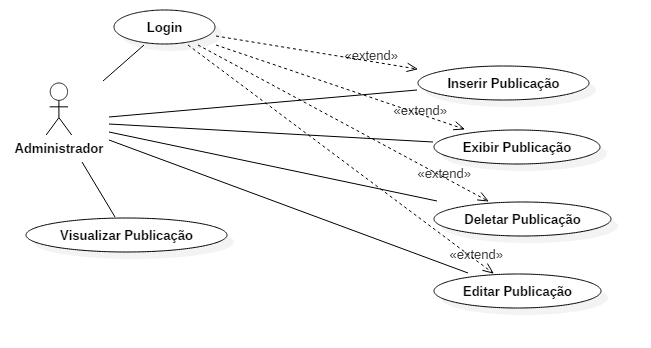
\includegraphics[scale=0.4]{figuras/casosDeUsoADM}
\caption{Casos de uso da ações do módulo administrador}
\label{fig:casosDeUsoADM}
\end{figure}

O acesso ao módulo é restrito, sendo necessário autenticação e para esse fim foi escolhido a ferramenta ``\textit{login} com o Facebook'', que a própria rede social disponibiliza como explicado na Seção \ref{sec:autenticacao}. Optou-se pelo uso dela, pois provê maior segurança, sendo baseada em sistemas criptográficos e também por facilitar o processo de recuperação de alguns dados básicos que são necessários para o processo de autenticação com o sistema. O diagrama de sequência que representa o processo de autenticação está representado na Figura \ref{fig:sequencialogin}.

\begin{figure}[H]
\centering
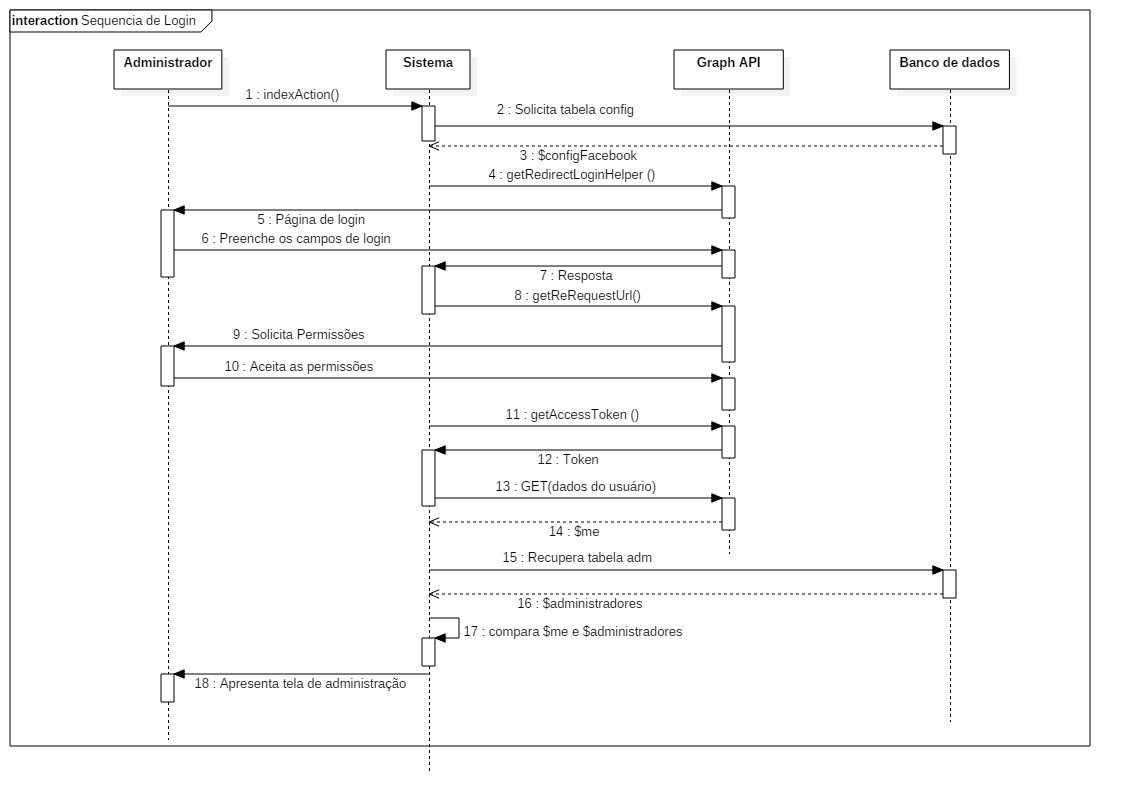
\includegraphics[scale=0.3]{figuras/sequencialogin}
\caption{Sequencia para efetivação de \textit{login}}
\label{fig:sequencialogin}
\end{figure}

A estruturação do banco de dados é composta por três tabelas, sendo mapeadas com as entidades ``config'', ``divulgacao'' e ``adm''. A função da tabela ``divulgacao'' é armazenar todos os objetos relacionados as divulgações que serão exibidas no cliente e no aplicativo. A tabela ``adm'' é usada para armazenar as informações referentes aos administradores do sistema. A tabela ``config'' é destinada a armazenar informações únicas para efetivação da comunicação entre aplicativo e Graph API.

\begin{figure}[H]
\centering
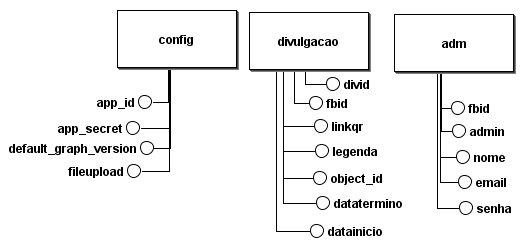
\includegraphics[scale=1.2]{figuras/entidaderelacionamento}
\caption{Modelo entidade e relacionamento}
\label{fig:casosDeUso}
\end{figure}

A Figura \ref{fig:diagramaclasseADM}, mostra a representação e o relacionamento entre as classes disponíveis no módulo. No diagrama de sequência \ref{fig:sequenciainserir} é exposta a sequência de uso das classes ao inserir uma nova publicação no sistema. 
\begin{figure}[H]
\centering
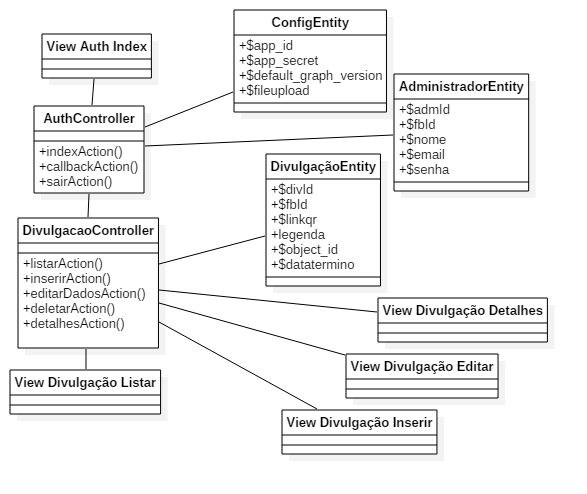
\includegraphics[scale=0.7]{figuras/diagramaclasseADM}
\caption{Diagrama de classe do módulo administrador}
\label{fig:diagramaclasseADM}
\end{figure}

 \begin{figure}[H]
\centering
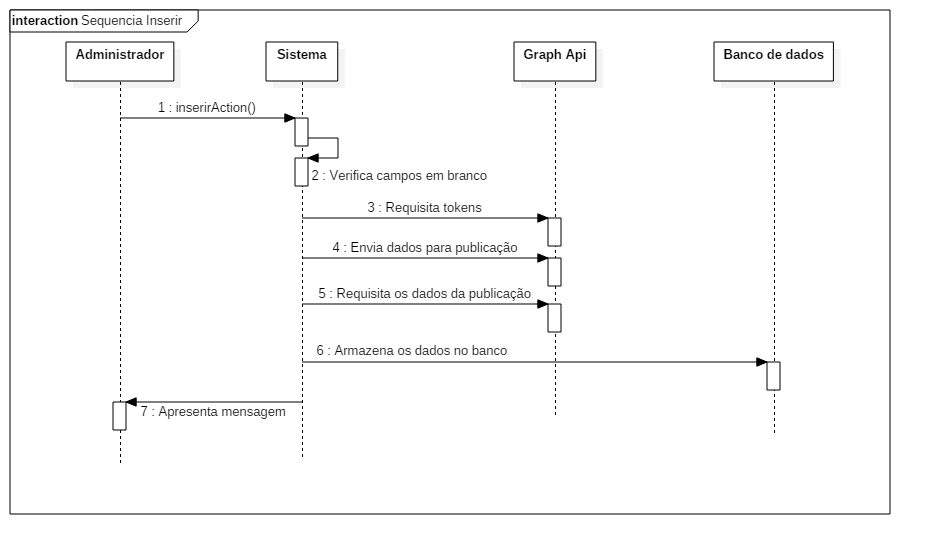
\includegraphics[scale=0.4]{figuras/sequenciainserir}
\caption{Diagrama de sequência para inserção}
\label{fig:sequenciainserir}
\end{figure}

Após a efetivação da autenticação, o usuário poderá ter acesso a todas as funcionalidades disponíveis no sistema, divididas entre as telas de ``inserir'' e ``Home''. A tela de inserir, é usada para criação de uma nova publicação, enquanto a tela Home oferece a opção de listar, detalhar, deletar e editar essa publicações que foram criadas.

A Figura \ref{fig:administrador1}, representa a visão do operador da tela de inserção, onde cada elemento da página está enumerado.

\begin{figure}[H]
\centering
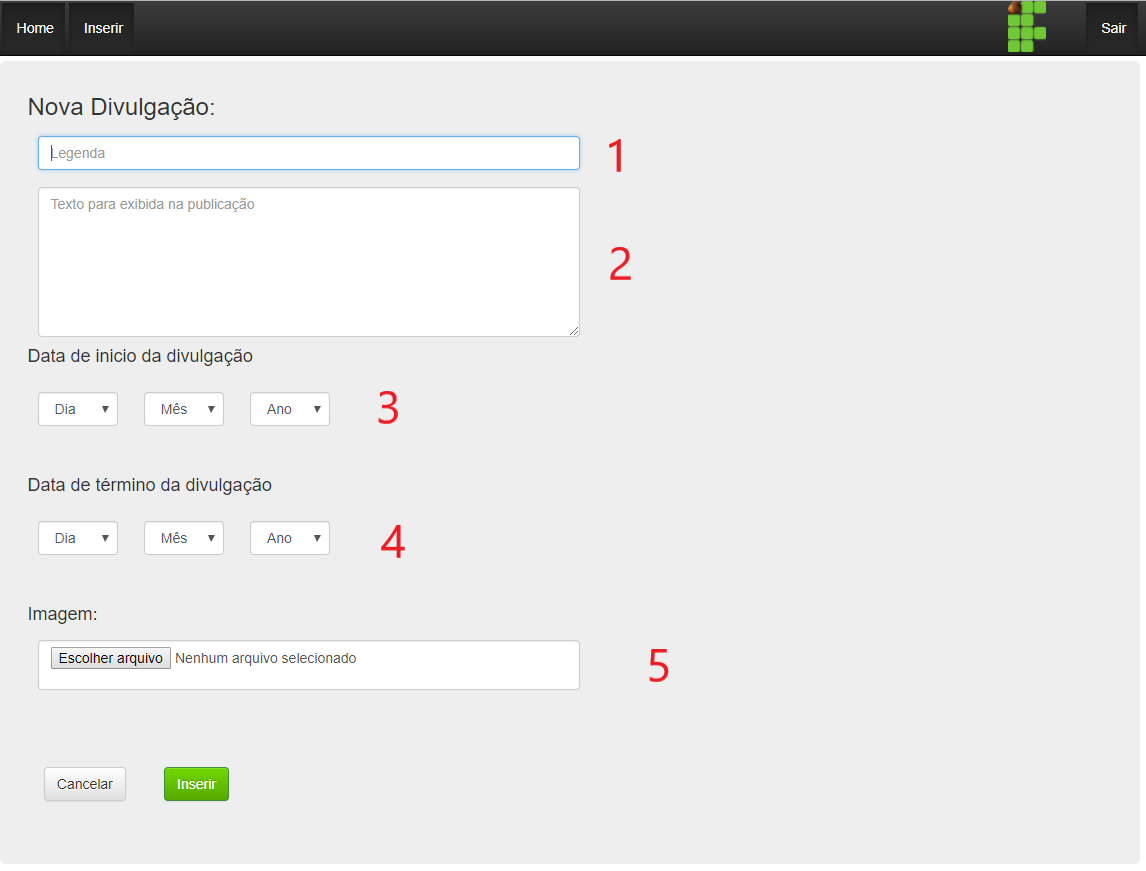
\includegraphics[scale=0.4]{figuras/administrador1}
\caption{Página de inserção do módulo administrador.}
\label{fig:administrador1}
\end{figure}

Os elementos presentes na tela de inserir são listados abaixo, juntamente com suas funcionalidades: 

\begin{enumerate}
   \item Legenda: É um campo de texto destinado a informação a ser repassada de forma sucinta e clara ao usuário final por intermédio cliente ou mobile. 
   \item Texto: É todo o texto que será enviado ao Facebook, contendo informações como descrição da publicação, data e horário da realização e um possível \textit{link} para acesso a mais informações. 
   \item Data de Início: É a data inicial em que a publicação começará a ser exibida no cliente e no mobile.
   \item Data de Término: É a data final em que a publicação deixará de ser exibida no cliente e no mobile.
   \item Imagem: Será a imagem enviada para o Facebook, para o cliente e para o mobile. Essa imagem pode ser um \textit{banner} de apresentação de um evento, por exemplo.
 \end{enumerate}

Todos os campos são de preenchimento obrigatório. O campo 5 é repassado para a API como parâmetro \textit{source}, já o campo 2 é repassado como parâmetro \textit{messagem}, os outros campos são enviados somente para o banco de dados.

Se durante o envio alguma das transações não forem efetivadas, será retornado a mensagem de erro na tela, assim como retornará a mensagem de sucesso, caso não ocorra nenhum erro.

O texto do campo 1 poderá conter letras ou números, entretanto possui a limitação máxima de 80 caracteres, isso é necessário para facilitar a leitura do usuário ao texto que será inserido, pois ele será armazenado no banco de dados e recuperado no módulo cliente para exibição.

Os outros campos não possuem limitação de caracteres, entretanto os campos 3, 4 e 5 possuem restrição de tipo de entrada, onde os campos 3 e 4 obrigatoriamente será um número inteiro e o campo 5, será um arquivo de imagem do tipo JPEG, JPG, GIF ou PNG.

Os campos 3 e 4 são botões do tipo dropdown, onde é preciso selecionar um dos valores que aparecem em cada um dos campos. Os possíveis valores para o campo ``dia'' vão de 1 a 31, os valores do campo ``mês'' vão de 1 a 12, enquanto os valores do campo ``ano'' irão do ano atual a dois anos seguintes.

A página ``Home'' é responsável por listar todas as publicações criadas, a visão do usuário será a mesma que representada na Figura \ref{fig:administrador2}. As funcionalidades de cada elemento da página são descritas logo abaixo. Essa é a página inicial do sistema, nela é possível ter acesso a página de inserção, listagem, detalhamento e ao botão excluir.

\begin{figure}[H]
\centering
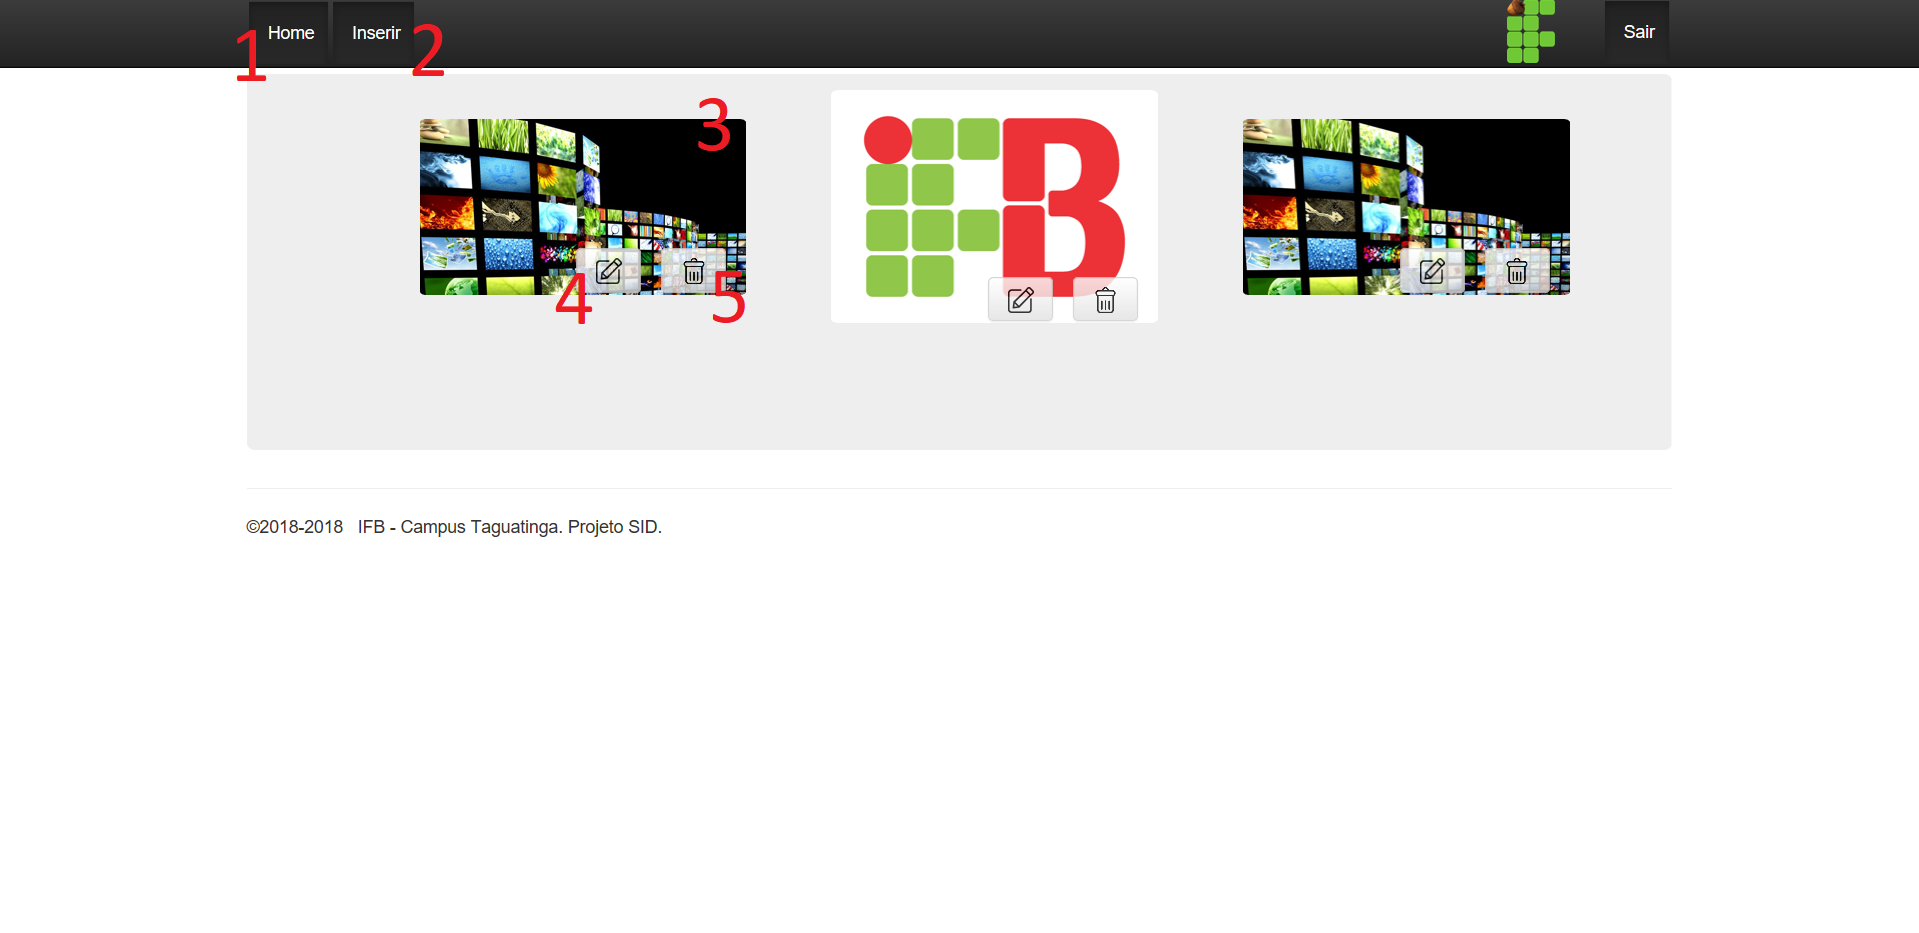
\includegraphics[width=\textwidth]{figuras/administrador2}
\caption{Página de listagem  do módulo administrador.}
\label{fig:administrador2}
\end{figure}

\begin{enumerate}
   \item Home: Botão para acesso a página inicial, onde são listadas todas as publicações criadas.
   \item Inserir: Botão para acesso a página de inserção.
   \item Detalhes: Ao clicar sobre a foto é possível obter dados específicos da publicação selecionada, tais como: Legenda, ID do autor, link de acesso a publicação, data de início, data de término, ID da publicação.
   \item Editar: Ao clicar no botão editar, será apresentado uma nova página edição dos dados específicos da publicação selecionada.
   \item Excluir: Exclui a publicação selecionada.
 \end{enumerate}

\subsection{Módulo API}
O módulo API faz parte do módulo administrador e possui a finalidade de recuperar os dados das publicações realizadas pelo administrador no Facebook, estruturá-los de forma que atendam a arquitetura REST e realizar o controle de alguns dados. Isso é crucial para que o módulo cliente e o aplicativo possam realizar requisições de solicitação ou envio de dados.

O controle de dados realizado pelo módulo API é indispensável para que conteúdos como comentários inadequados não sejam exibidos. Para esse controle é efetuado uma varredura de todos os usuários que curtiram cada comentários da publicação, caso seja encontrado a curtida de um dos administradores cadastrados no banco de dados o comentário é aprovado para ser exibido.

Além disso, as requisições para esse módulo devem seguir uma sintaxe de acordo com os dados desejados. Como mostra a Listagem \ref{lst:bd}, onde é requisitado as informações das publicações presentes no banco.

\begin{lstlisting}[caption={Requisitando dados para divulgação},label={lst:bd}]
	http://{IP DO SERVIDOR}:{PORTA}/bd
\end{lstlisting}

A resposta para a solicitação da Listagem \ref{lst:bd} é um arquivo do tipo JSON contendo o conteúdo apresentado no Listagem \ref{lst:retornobd}. O uso de cada um dos itens será explicado na Seção \ref{sec:cliente}.

\begin{lstlisting}[caption={Retorno da requisição \ref{lst:bd}},label={lst:retornobd}]
{
	0:[
		"bd": [
			"linkqr": {LINK DA DIVULGACAO}
			"legenda": {LEGENDA QUE SERA EXIBIDA}		
		],
		"comentarios": null,
		"imagem": []
	1:[
		"bd": [
			"linkqr": {LINK DA DIVULGACAO}
			"legenda": {LEGENDA QUE SERA EXIBIDA}
		],
		"comentarios": [
			0: [
				"created_time": {DATA DA CIRACAO},
				"from": [
					"nome": {NOME DO USUARIO},
					"id": {ID DO USUARIO}
				],
				"message": {MENSAGEM APRESENTADA},
				"id": {ID DA PUBLICACAO},
				"urlFoto": {URL DA FOTO DE PERFIL DO USUARIO}
			],
			1: [
				"created_time": {DATA DA CIRACAO},
				"from": [
					"nome": {NOME DO USUARIO},
					"id": {ID DO USUARIO}
				],
				"message": {MENSAGEM APRESENTADA},
				"id": {ID DA PUBLICACAO},
				"urlFoto": {URL DA FOTO DE PERFIL DO USUARIO}
			]
		],
		"imagem": {IMAGEM DE EXIBICAO, CODIFICADA}
	]
}
\end{lstlisting}

A propriedade `bd', contém uma \textit{array} de duas posições, contendo 2 \textit{strings}, sendo elas legenda e link. Esses dados foram armazenados pelo servidor no banco de dados, na criação da publicação. A propriedade `comentarios' é um array de \textit{strings} que pode possuir zero ou mais itens. Cada item representa um comentário da publicação, cada qual contendo data de criação, autor, foto de perfil e identificador do comentário. Já a 'imagem' é uma \textit{string} que representa uma imagem codificada em base64 a ser decodificada pelo módulo cliente.

O módulo API tem a função de, em conjunto com o banco de dados, realizar a simulação de um sistema de gestão acadêmico, sendo possível consultar alguns dados através de requisições. Os dados que podem ser recuperados, variam de acordo com a sintaxe utilizada.

É possível requisitar diversos dados distintos ou todos eles juntos. 
No Listagem \ref{lst:todos} é feito a requisição de todos os dados armazenados, que retornará um JSON de diversas posições, onde cada posição representa um mensagem enviada por um professor.
\begin{lstlisting}[caption={Requisitar todos os dados},label={lst:todos}]
	http://{IP DO SERVIDOR}/mobile
\end{lstlisting}

\begin{lstlisting}[caption={Retorno da requisição \ref{lst:todos}},label={lst:retornotodos}]
	0:[
		"id_mensagem": {NUMERO DA MENSAGEM NO SERVIDOR},
		"matricula_professor": {MATRICULA DO PROFESSOR},
		"nome_professor": {NOME DO PROFESSOR QUE ENVIOU},
		"id_turma": {IDENTIFICACAO DA TURMA},
		"mensagem": {MENSAGEM ENCAMINHADA PELO PROFESSOR}
	],
	1:[		
		"id_mensagem": {NUMERO DA MENSAGEM NO SERVIDOR},
		"matricula_professor": {MATRICULA DO PROFESSOR},
		"nome_professor": {NOME DO PROFESSOR QUE ENVIOU},
		"id_turma": {IDENTIFICACAO DA TURMA},
		"mensagem": {MENSAGEM ENCAMINHADA PELO PROFESSOR}
	]
\end{lstlisting}

A inclusão de um novo parâmetro na requisição da Listagem \ref{lst:todos} torna a busca mais específica. Por exemplo, pode ser usado ``/professores'', ``/alunos/'', ``/turmas/'' ou ``/mensagens/'', isso retornará um JSON contendo uma lista somente com os dados solicitados. Na Listagem \ref{lst:professores}, o retorno será uma lista com os dados de todos os professores cadastrados como mostra a Listagem \ref{lst:retornoprofessores}.

\begin{lstlisting}[caption={Requisitar lista de dados especifica},label={lst:professores}]
	http://{IP DO SERVIDOR}/mobile/professores/
\end{lstlisting}

\begin{lstlisting}[caption={Retorno da requisição \ref{lst:bd}},label={lst:retornoprofessores}]
	0:[
		"matricula": {MATRICULA DO PROFESSOR},
		"nome": {NOME DO PROFESSOR QUE ENVIOU},
		"senha": {SENHA CRIPTOGRAFADA}
	],
	1:[		
		"matricula": {MATRICULA DO PROFESSOR},
		"nome": {NOME DO PROFESSOR QUE ENVIOU},
		"senha": {SENHA CRIPTOGRAFADA}
	]
\end{lstlisting}

O diagrama de classe que representa esse módulo é descrito na Figura \ref{fig:diagramaclasseAPI}. Cada uma das classes é usada para uma determinada requisição.
\begin{figure}[H]
\centering
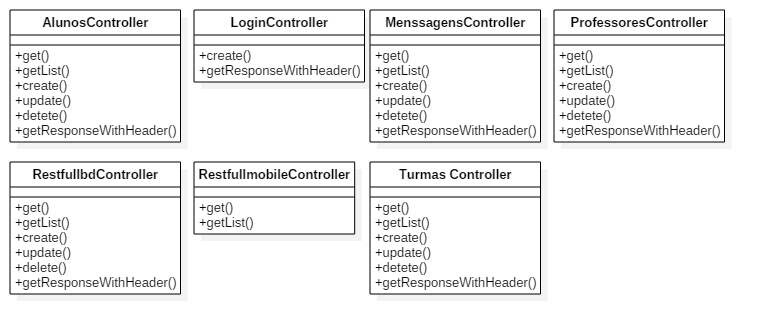
\includegraphics[scale=0.5]{figuras/diagramaclasseAPI}
\caption{Diagrama de classe do módulo API}
\label{fig:diagramaclasseAPI}
\end{figure}

\section{Módulo Cliente}
\label{sec:cliente}
O modulo cliente tem a função de apresentar as divulgações de maneira atrativa, intuitiva e dinâmica para o usuário. O seu caso de uso é apresentado na Figura \ref{fig:casosDeUsoCliente}. A estrutura e organização do que será apresentado, está disposto na Figura \ref{fig:cliente1} e o seu diagrama de classe é apresentado na Figura \ref{fig:diagramaclasseCLIENTE}.

\begin{figure}[H]
\centering
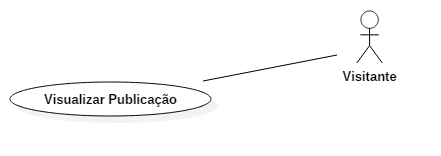
\includegraphics[scale=0.6]{figuras/CasosDeUsoCliente}
\caption{Casos de uso da ações do módulo cliente}
\label{fig:casosDeUsoCliente}
\end{figure} 

\begin{figure}[H]
\centering
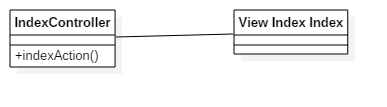
\includegraphics[scale=0.4]{figuras/diagramaclasseCLIENTE}
\caption{Diagrama de classe do módulo cliente}
\label{fig:diagramaclasseCLIENTE}
\end{figure}

Os elementos que compõem a página que será apresentada são divididos em cinco itens, que estão descritos abaixo.

\begin{enumerate}
   \item Imagem: O conteúdo poderá ser apresentado como uma imagem estática ou como GIF (imagem com animação), não oferecendo suporte a vídeos, até o momento, mas que poderá ser implementado em versões futuras. 
   \item Legenda: A legenda é apresentada em movimento linear da direita para a esquerda, possibilitando a leitura de forma dinâmica de toda a frase.
   \item QR Code: Imagem, que por meio de um aplicativo celular, possibilita a leitura que contém o \textit{link} de acesso a publicação publicada na rede social Facebook.
   \item Horário: Relógio que apresentará a data e hora atual.  
   \item Comentários: Espaço que será apresentado comentários publicados e devidamente moderados.
 \end{enumerate}
  
\begin{figure}[H]
\centering
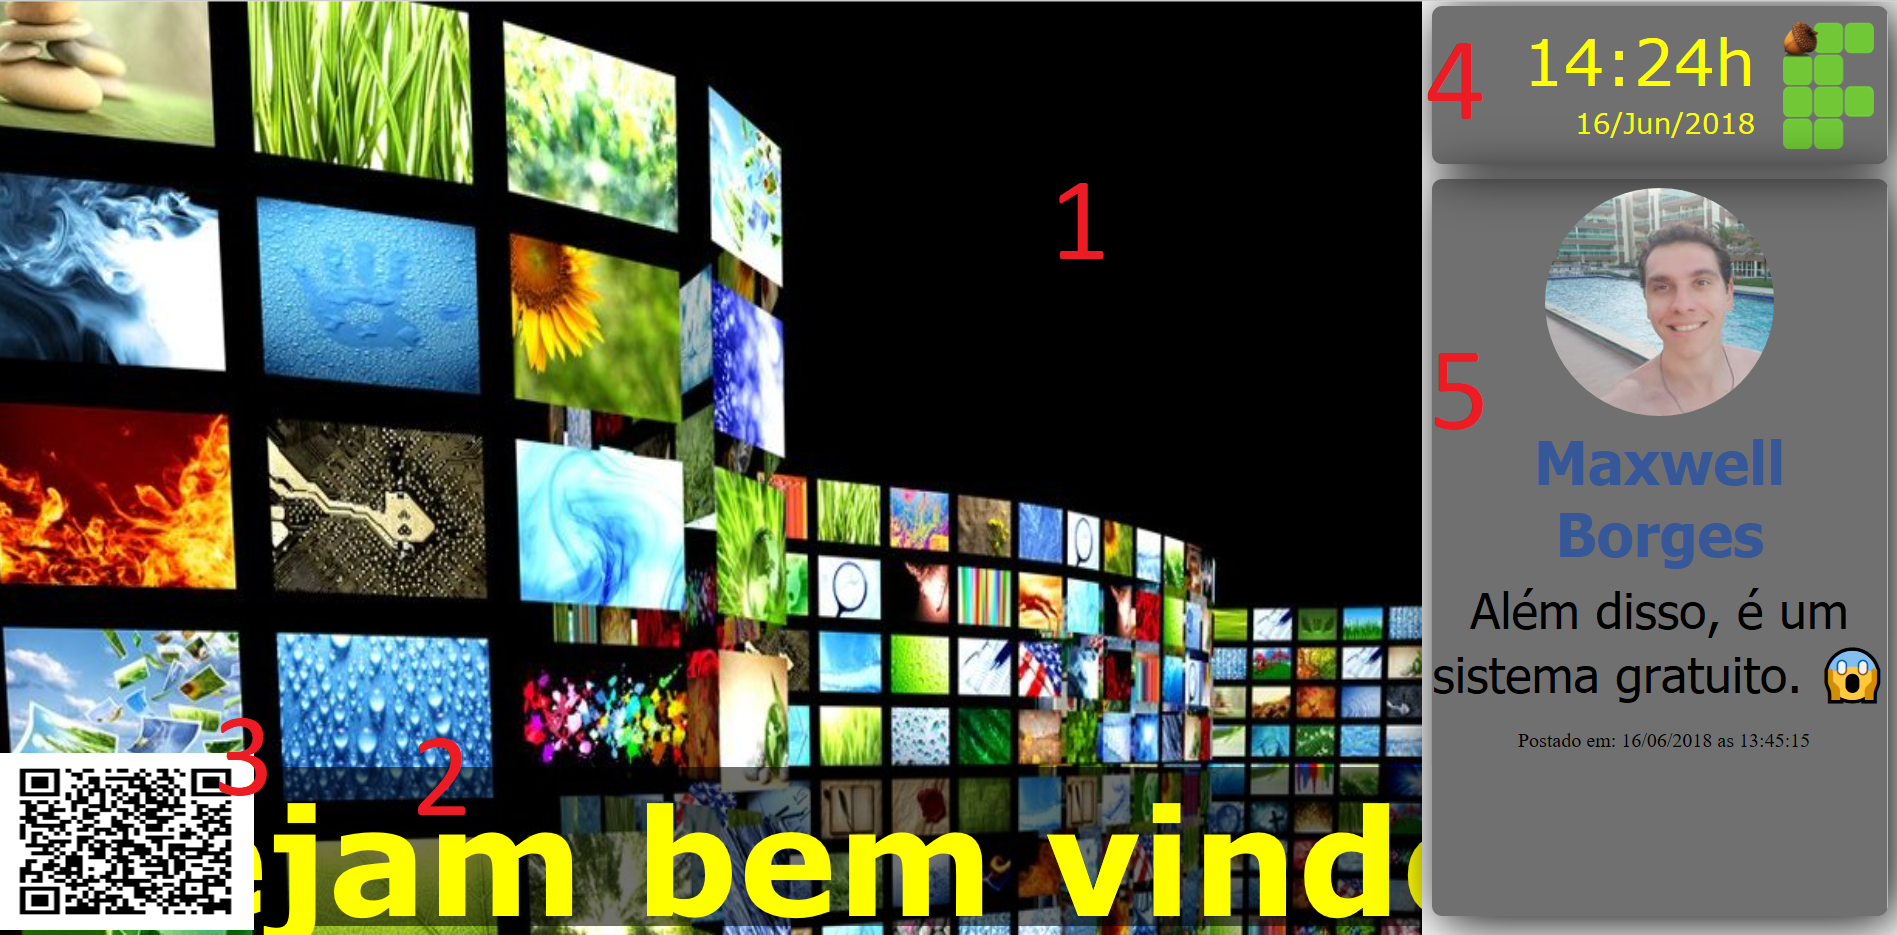
\includegraphics[scale=0.3]{figuras/cliente1}
\caption{Página do cliente}
\label{fig:cliente1}
\end{figure}

Consumindo uma API REST com requisições do tipo GET feitas a URL da Listagem \ref{lst:bd}, o módulo cliente receberá como resposta um JSON, contendo o número de posições equivalentes ao número de publicações válidas. Cada posição desse JSON terá três variáveis, são elas: ``bd'',``comentarios'' e ``imagem'', como apresentado na Listagem \ref{lst:retornobd}. 

O conteúdo recuperado da variável ``bd'', será apresentado nos itens 2 e 3, respectivamente. Já o conteúdo recuperado da variável ``comentarios'' será apresentado no item 5. Enquanto os da variável ``imagem'', será descriptografado e apresentado em forma de imagem no item 1.

O campo 5 irá apresentar 5 elementos recuperados na variável ``comentarios''. Esses elementos serão: a imagem de perfil, o nome, o comentário, a data e a hora da publicação do comentário feito pelo usuário. Antes da apresentação das informações de comentários, é escolhido um número randômico que representará a posição do array do comentário que será apresentado.

\section{Aplicativo Mobile}
Desenvolvido com auxílio dos \textit{Frameworks} Cordova, Framework7 e Dom. O aplicativo \textit{mobile} é responsável por apresentar de forma pública as divulgações, assim como o módulo cliente, com algumas funcionalidades a mais que são restritas.

As funcionalidades adicionais do aplicativo são as de disponibilizar uma melhor forma de comunicação entre professores e alunos, necessitando apenas de autenticação. Para autenticação é preciso que o aluno ou o professor tenha uma matrícula e senha cadastradas no banco.

Os casos de uso do aplicativo são demostrados na Figura \ref{fig:casosdeusomobile}, enquanto o modelo entidade e relacionamento é apresentado na Figura \ref{fig:entidaderelacionamentomobile}.
\begin{figure}[H]
\centering
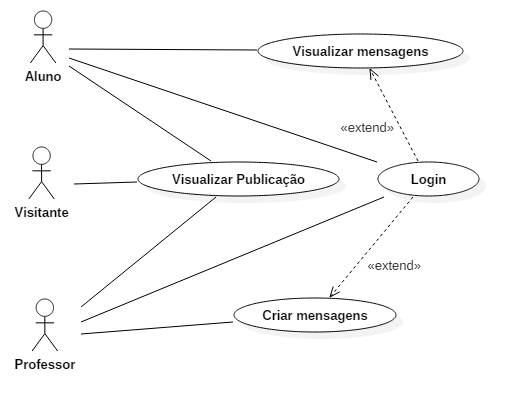
\includegraphics[scale=0.4]{figuras/CasosDeUsoMobile}
\caption{Casos de uso aplicativo móvel.}
\label{fig:casosdeusomobile}
\end{figure}

\begin{figure}[H]
\centering
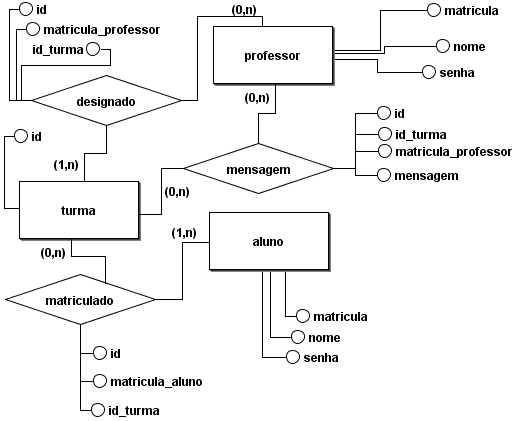
\includegraphics[scale=0.8]{figuras/entidaderelacionamentomobile}
\caption{Modelo entidade e relacionamento aplicativo móvel.}
\label{fig:entidaderelacionamentomobile}
\end{figure}

O aplicativo contará com três telas distintas que serão a tela inicial, a tela do aluno e a tela do professor. Em cada tela o sistema faz requisição de um serviço diferente para o módulo API. Na tela inicial é feito a requisição GET a Listagem \ref{lst:bd}, na tela do aluno é feito a requisição GET a Listagem \ref{lst:todos} e na tela do professor é feito um POST a Listagem \ref{lst:incluirmensagem},

\begin{lstlisting}[caption={Incluir novas mensagens},label={lst:incluirmensagem}]
	http://{IP DO SERVIDOR}/mensagens/
\end{lstlisting}

A tela inicial será apresentada como na Figura \ref{fig:mobile1}, exibindo o nome do SID e o botão de login na parte superior e as informações das publicações válidas, que foram requisitadas do módulo API, no restante da tela.
\begin{figure}[H]
\centering
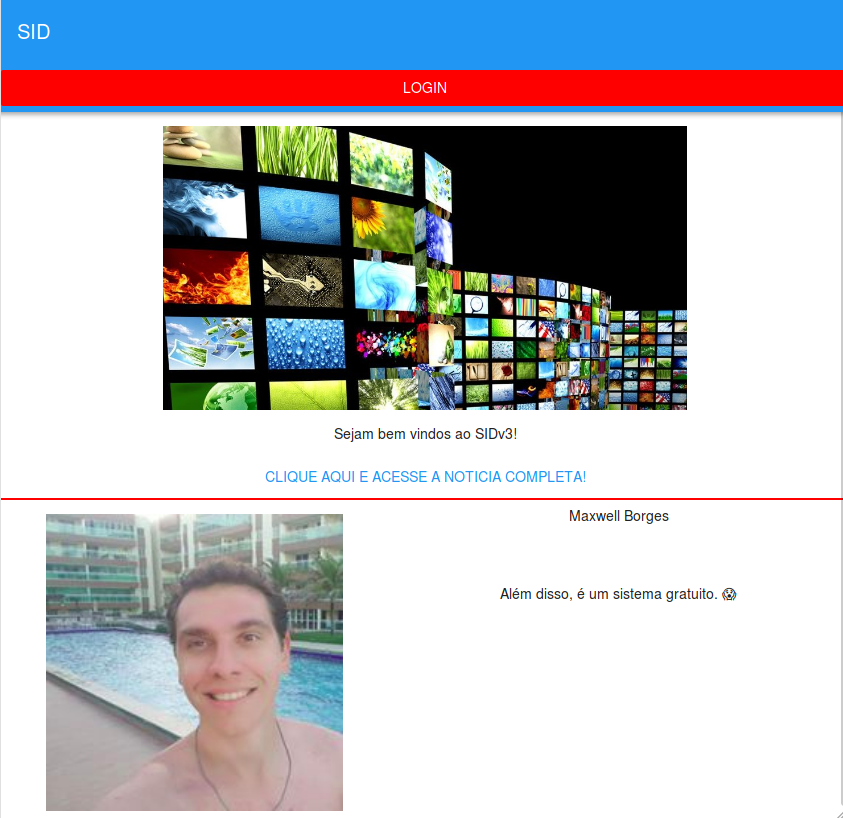
\includegraphics[scale=0.5]{figuras/mobile1}
\caption{Página de inserção no módulo administrador.}
\label{fig:mobile1}
\end{figure}

A funcionalidade de login é indispensável para que alunos e professores efetuem a autenticação e possam acessar as páginas restritas destinadas a cada um.

A tela do aluno será apresentada como na Figura \ref{fig:mobile2}, após o login, será apresentado ao aluno todas as mensagens que o aluno possui em ordem cronológica da mais nova para a mais antiga. Os campos apresentados são os de professor, turma e mensagem, separando cada item por blocos.

\begin{figure}[H]
\centering
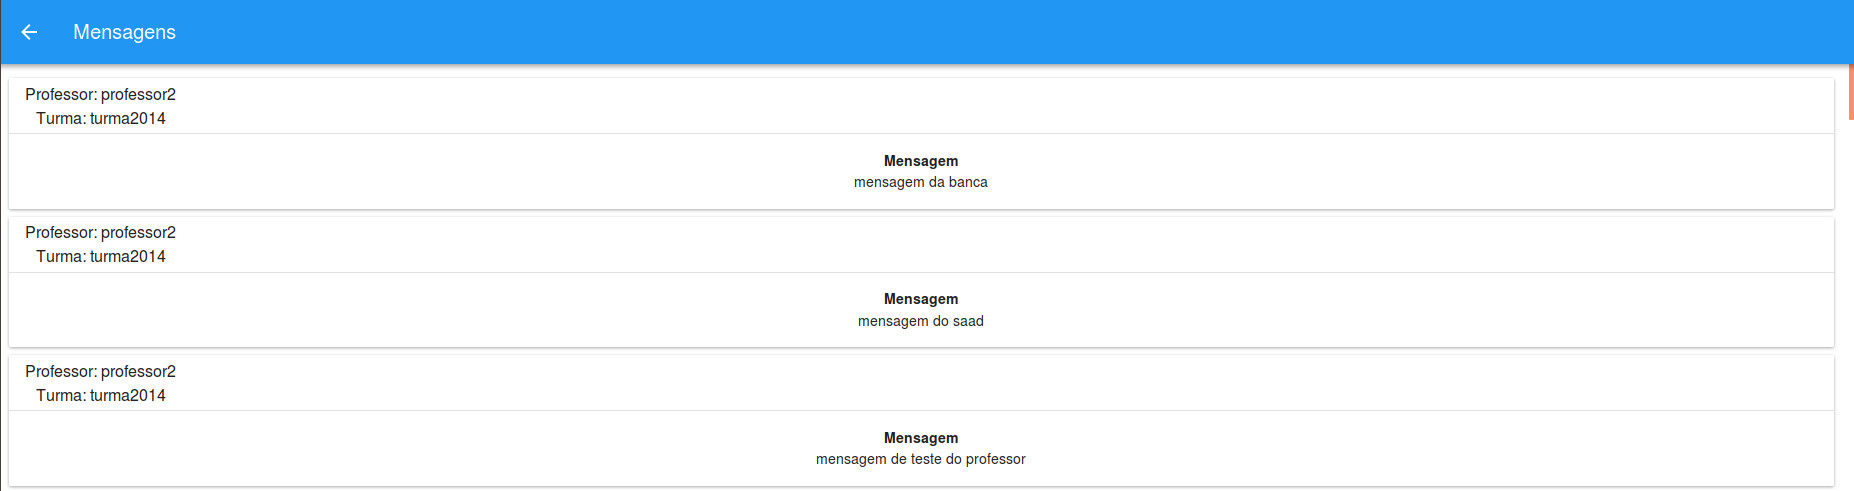
\includegraphics[scale=0.6]{figuras/mobile3}
\caption{Página do Aluno.}
\label{fig:mobile2}
\end{figure}

Já a tela do professor será apresentada conforme a Figura \ref{fig:mobile3}, após o login, será apresentado ao professor a matricula dele, a lista de turmas que ele leciona e uma caixa de texto que o professor usará para digitar a mensagem.

\begin{figure}[H]
\centering
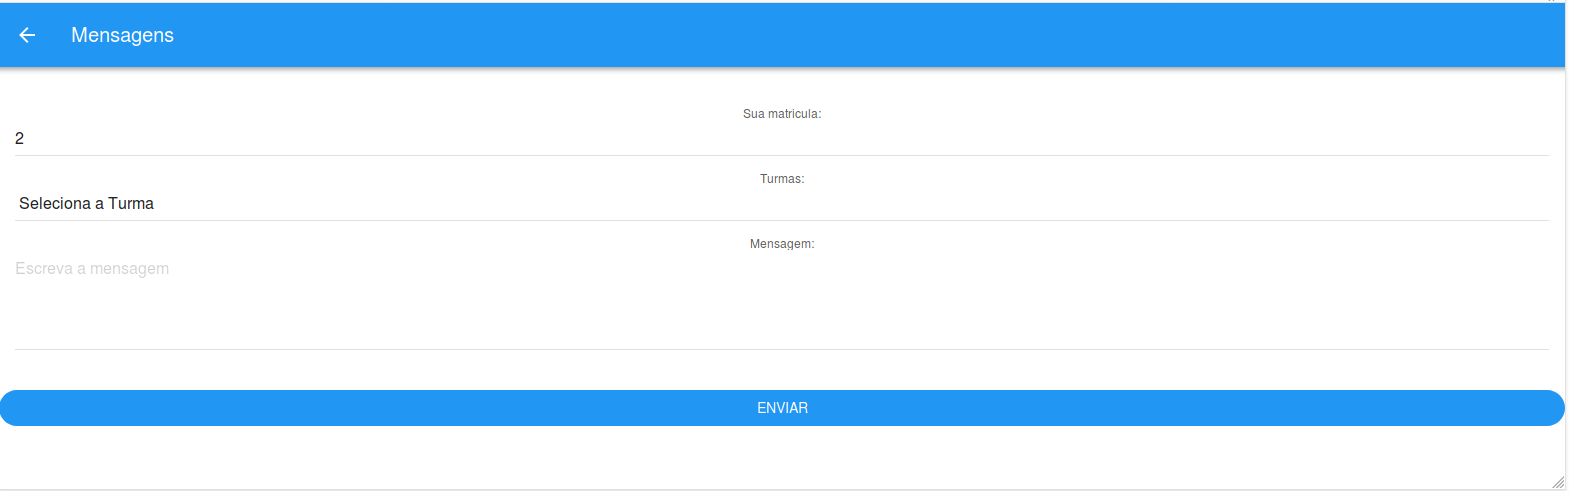
\includegraphics[scale=0.5]{figuras/mobile2}
\caption{Página do professor.}
\label{fig:mobile3}
\end{figure}

Todos os campos são de preenchimento obrigatório e caso algum erro ocorra no processo de envio, o sistema apresentará um notificação para o professor com o erro ocorrido.

\section{Integração}
A integração entre o sistema e o Facebook se dá com o uso da Graph API. Ferramenta disponibilizada pela rede social para que feita a integração de sistemas externos a rede social Facebook.

Com o uso dela, pode-se recuperar os mais diversos dados de acordo com as permissões que são concedidas.

\subsection{\textit{login}, \textit{token} de acesso e permissões}
Para autenticação e efetivação de todas as requisições feitas pelo módulo administrador para o Facebook é necessário que um \textit{login} seja feito. Para isso, é utilizado a ferramenta de ``\textit{login} do Facebook''  que é disponibilizada pela rede social.

A ferramenta de ``\textit{login} do Facebook'' que é disponibilizada pelo mesmo, oferece um botão que pode ser colocado na página que possui a finalidade de iniciar o processo de login. Após ser clicado é efetuado o processo de login conforme segue padrão estabelecido, solicitando as credenciais cadastradas na rede social, com isso é feito a requisição com as permissões necessárias conforme Listagem \ref{lst:solicitacaologin}.

No processo de \textit{login} são solicitados as permissões necessárias para que o sistema funcione, essas permissões são a “email”, “manage\underline{{ }}pages” e “publish\underline{{ }}pages”, sendo obrigatório o aceite para acesso ao sistema. Usadas respectivamente para que seja possível a identificação do usuário do SID, para recuperar as permissões de acesso a página e a última para permitir que aplicativos publiquem na página \cite{facebook2018a}.

Após a efetivação do login o sistema realiza a requisição da Listagem \ref{lst:permissoesaceitas} para verificar as permissões que o usuário concedeu, onde o retorno será um JSON contendo todas as permissões concedidas.

\begin{lstlisting}[caption={Permissões concedidas},label={lst:permissoesaceitas}]
  	$response = $fb->get(
    	'/me/permissions',
		'{access-token}'
	);
	
	$graphNode = $response->getGraphNode();
\end{lstlisting}

Então o sistema compara as permissões aceitas com as permissões necessárias e caso alguma não esteja presente, o acesso é negado, retornando para a página de login e apresentado a mensagem de erro para o usuário.

A existência de um usuário vinculado a rede social é irrefutável, pois existe a necessidade da página apresentar qual o perfil está realizando a ação, além da necessidade de moderação dos comentários que serão exibidos.  Além disso, para efetivação de todas as requisições feitas pelo módulo administrador para o Facebook, seja ela para requisitar informações das publicações ou realizar uma nova publicação, é usando o \textit{token} de acesso de usuário, que é obtido no processo de login, conforme Listagem \ref{lst:tokenUsuario}.

Entretanto, para o acesso é indispensável também que o um usuário esteja cadastrado no banco de dados do SID. Essa ação é necessária para que somente usuários autorizados possam realizar alteração na página usando o sistema.

Após o login, algumas informações usadas são guardadas na sessão do usuário, para usos posteriores. Porém, todo o processo de armazenamento de informações, envios ao Facebook e retornos de solicitações não devem ser visíveis ao usuário. 

\subsection{Publicar}
Todas as publicações que são realizadas no Facebook usando o SID são feitas ao nó ``/photo'', onde a cada nova publicação será gerado um ID para ela e terá a mesma estrutura de uma imagem postada por um usuário convencional desta rede social.

Na criação de uma nova publicação, usando o SID, são passados para a Graph API dois parâmetros para inserção através do método POST, conforme Listagem \ref{lst:requisicao9}. O primeiro deles é “message”, onde será passado o texto que será exibido na publicação e o outro é “source”, onde será passado a imagem para ser exibida juntamente com o texto. Para envio de imagem para a rede social, é necessário passar na imagem como parâmetro o método “fileToUpload” conforme Listagem \ref{lst:appesdk}. 

Alguns dos elementos que são solicitados pela aplicação na criação de uma nova publicação são omitidos no envio para o Facebook, pois esses dados serão usados apenas para serem armazenados no banco para uso do módulo cliente. Os elementos omitidos são os campos data de início, a data de termino e a legenda. 

A Figura \ref{fig:imgfacebook1} apresenta como fica uma publicação no Facebook após o uso do SID para criação da mesma, enquanto a Figura \ref{fig:cliente1} apresenta como será exibido no módulo cliente. Nela são apresentadas informações como quem realizou a publicação, o texto e a imagem que foram informados durante a criação da divulgação pelo SID.

\begin{figure}[H]
\centering
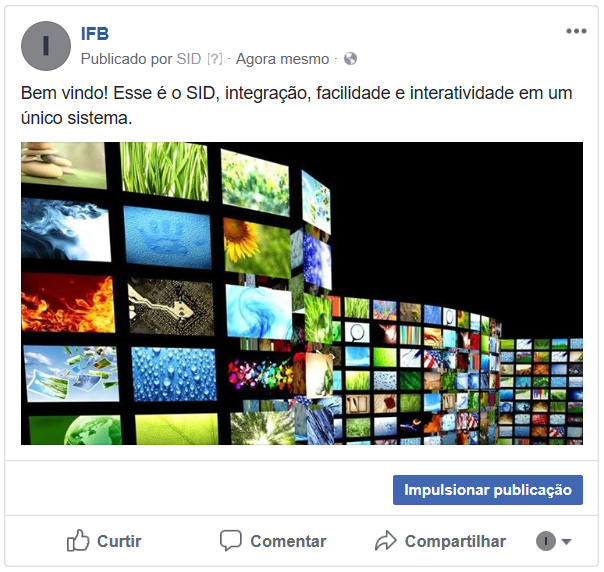
\includegraphics[scale=0.8]{figuras/imgfacebook1}
\caption{Divulgação enviada ao Facebook com auxílio do SID}
\label{fig:imgfacebook1}
\end{figure}


\subsection{Requisição}
Usando o ID da foto é possível recuperar informações das arestas, que podem ser a URL, os comentários e as curtidas conforme Listagem \ref{lst:requisicao8}. 

Esse recurso é utilizado para recuperar os mais diversos elementos que as permissões concedidas autorizam, entre os elementos recuperados estão o endereço da publicação, os comentários, curtidas e a imagem de perfil que serão apresentados respectivamente nos campos destinados ao QR Code e na coluna de comentários do módulo cliente.

A URL da publicação que é criada, é armazenada no banco de dados no momento da criação da mesma pelo modulo administrador. A requisição segue a Listagem \ref{lst:requisitarurl}.

\begin{lstlisting}[caption={Foto de usuário},label={lst:requisitarurl}]
  	$response = $fb->get(
    	'/{ID PUBLICACAO}?fields=link',
		'{access-token}'
	);
	
	$graphNode = $response->getGraphNode();
\end{lstlisting}

A recuperação dos outros dados necessários é feito pelo módulo API, onde ele realiza requisições a Graph. As requisições feitas pelo módulo são para recuperação de comentários da Listagem \ref{lst:comentariosPostagem}, de curtidas desses comentários, conforme Listagem \ref{lst:curtidasComentario} e foto de perfil do usuário que realizou o comentário conforme Listagem \ref{lst:fotousuario}.

\begin{lstlisting}[caption={Foto de usuário},label={lst:fotousuario}]
  	$response = $fb->get(
    	'/{ID USUARIO}?fields=picture',
		'{access-token}'
	);
	
	$graphNode = $response->getGraphNode();
\end{lstlisting}

A recuperação dos comentários e da foto do perfil do usuário que publicou cada comentário é crucial para que essa informação seja exibida no módulo cliente, no elemento 5, conforme a Figura \ref{fig:cliente1}.

A recuperação de curtidas é necessária para que possa ser feito a moderação dos comentários a serem exibidos. A moderação é feita de forma a verificar o ID de todos os usuários que curtiram cada comentário a fim de verificar se algum dos IDs encontrados é o ID do administrador que está cadastrado no banco.

Os comentários que possuem a curtida do administrador é registrado para exibição no elemento 5 da Figura \ref{fig:cliente1}.

\section{Possível solução para Implantação - Raspberry}
Para viabilizar uma implementação barata ao \textit{Campus} Taguatinga, computadores Raspberry Pi podem ser utilizados.

Teste do \cite{aristotelous2016} apresenta a possibilidade de se ter um servidor completamente funcional com sistema operacional Linux por um equipamento de 35\$, possibilitando a criação de um servidor, por exemplo de um repositório na nuvem com um baixo custo, flexibilidade e eficiência energética. 

Para \cite{cusick2014}, placas de circuito oferecem vantagens como: Uso de pouco espaço; Desempenho significante com baixo custo e consumo; Suporte a diversas soluções de software, oferecendo múltiplas opções de interface com uma variante do Linux. 

Portanto, este tipo de dispositivo provê diversos benefícios que podem ser de grande importância na escolha de um sistema para implementação do módulo cliente do SID.
\chapter[Resultados]{Resultados}
A ideia anterior do SIDv2, desenvolvido por \cite{sobrinho2017}, era a de um sistema inteligente de divulgação, entretanto, no presente trabalho a ideia foi alterada para um sistema integrado de divulgação. Isso se deu pelo fato de o sistema não possuir nenhum tipo de inteligência própria e sim realizar a integração entre redes sociais e usuário.

O SID passou por diversas reformulações de suas concepções iniciais. Em sua versão anterior, ele possuía integração bastante limitada, nenhum tipo de aplicativo mobile para melhor interação acadêmica e pouca interatividade do sistema com o usuário e vice-versa. Então, no presente trabalho foi implementado toda a integração com o Facebook, melhorado a interação com o usuário, além da criação de um protótipo \textit{mobile}.

O presente trabalho apresenta a terceira versão do SID, com melhorias significantes como as apresentadas no Capítulo \ref{cap:sid}, estando pronto para implantação de modo a servir de aparato ao campus no processo de veiculação de informações.

Por falta de uma documentação anterior, foi necessário a criação de uma extensa documentação do software de modo a possibilitar futuras modificações e melhorias de maneira fácil.

No módulo administrador, foi possível alcançar todos os objetivos desejados, ficando responsável por todo o processamento e gerenciamento das informações no banco de dados. A partir dele é possível inserir, listar, deletar e editar as informações que servirão para que módulo API forneça os dados conforme a estrutura de uma arquitetura REST, permitindo que outras aplicações futuramente venham a consumir esta API.

Além disso, foi implementado uma verificação de segurança no processo de login que não existia no SIDv2, onde qualquer usuário cadastrado poderia acessar a aplicação. Entretanto, algumas funcionalidades oferecidas pelo módulo só estão disponíveis se forem concedidas algumas permissões específicas. Portanto, o login no módulo só é realizado caso todas as permissões solicitadas sejam aceitas.

O submódulo API, parte do módulo administrador, é estruturado de acordo com a arquitetura REST, com a capacidade de realizar um CRUD nas publicações e nas mensagens entre professor aluno.

Este submódulo foi implementado com duas funcionalidades distintas. A primeira é obter os dados do armazenados no banco e realizar as chamadas a Graph para obter os dados dos comentários das publicações que serão exibidas e organizar esses dados para que sejam enviados. A segunda, é servir de aparato ao aplicativo, para que ele possa simular o consumo de uma API externa. 

O módulo cliente do SID ficou estruturado e pronto para ser implantado e executado em diversos dispositivos, bastando o mesmo possuir um navegador de paginas \textit{WEB} e conexão constante a internet para que sejam realizadas as consultas HTTP. Essa facilidade é possível graças a implementação em arquitetura cliente-servidor, esse arquitetura foi proposta para que o módulo consumisse poucos recursos, permitindo o uso de dispositivos que dispõem de uma grande eficiência energética, como: \textit{Raspberry} PI, \textit{BoxTVs} ou até mesmo em sistemas integrados as próprias \textit{smartTvs}.

No protótipo do aplicativo mobile, foi implementado a funcionalidade de consumo de uma REST API fictícia, simulando o Sistema de Gestão Acadêmica do IFB, para exibição das divulgações e um sistema de comunicação interna entre professores e alunos, onde é necessário um login criado de maneira fictícia para simulação de um sistema acadêmico. necessitando apenas da liberação dos dados do SGA para autenticação do sistema e a adaptação das consultas feitas a esta API.

Na busca de soluções que seguem a ideia de criação de publicação para apresentação em dispositivos externos, foram encontradas diversas ferramentas com essa finalidade, todas elas usando o conceito de arquitetura cliente-servidor, as que apresentaram melhores funcionalidades foram a OOZO, a MangoSings, o SID versão 2, a Screenly e a XIBO.

O OOZO, apresentado na sessão \ref{sec:oozo}, é um sistema pago, porém possui uma versão gratuita com acesso limitado aos recursos oferecidos. Ele oferece suporte a multiplataformas, controle WEB, integração a redes sociais e acesso a publicações via QRCode. Apresentando duas limitações, uma é no que tange a integração com as redes sociais, onde é possível apenas recuperar e deletar publicações, a outra limitação está no acesso as divulgações por dispositivo móvel, onde é necessário o uso de navegadores \textit{WEB}. 

A MangoSigns, apresentado na sessão \ref{sec:mango}, é um sistema pago que possui uma versão gratuita com acesso limitado. A ferramenta possui acesso multiplataformas, inclusive móvel, diversos temas para apresentação e integração com as redes sociais. Possuindo a limitação da integração está disponível apenas na versão paga, além de ser possível apenas recuperar as publicações.

O SID versão 2, apresentado na sessão \ref{sec:sid}, é um sistema gratuito, que possui acesso somente \textit{WEB}, aceso a publicação via QRCode e integração as redes sociais. Nele é possível apenas realizar publicação da página de perfil do usuário, não sendo possível recuperar nenhum dado.

O Screenly, além de usar um aplicativo proprietário, necessitando de um \textit{raspberry}, ele não possui aplicativo \textit{mobile} e nenhuma forma de integração com as redes sociais.

Já o Xibo, apesar de ser uma ferramenta gratuita, não possui aplicativo mobile e nenhuma integração com as redes sociais. 

Comparando cada uma das ferramentas encontradas com o SIDv3 é possível notar diversas funcionalidades que não estão presentes, são limitadas ou não são gratuitas, portanto diversos pontos que são considerados como essenciais e foram implementados no SIDv3, as ferramentas apresentadas não suportam.

Entre esses pontos, está a visualização das publicações por meio de um aplicativo móvel, onde com exceção do MangoSings, nenhum dos sistemas ofereciam um aplicativo para \textit{smartphones}, necessitando de um dispositivo que possuísse um navegador WEB para acesso.

Outro ponto é o de integração com as redes sociais, nenhum das solução analisadas realizavam uma integração tão completa quanto ao do SIDv3, como a possibilidade de criação de novas publicações, recupeção de comentários, curtidas e fotos de perfil, além do filtro de comentários a serem exibidos. 

Além disso, nenhum deles possuía um aplicativo que realiza a integração com um sistema acadêmico, para integração entre professores e alunos.

A tabela \ref{tlb:comparacaoresultados} tem o intuito de fazer um comparativo entre os sistemas apresentados, agora com inclusão do SID em sua terceira versão, comparando algumas das funcionalidades consideradas importantes para sistemas que trabalham com a implantação de sinalização digital e \textit{maketing} digital, na qual seus elementos comparativos são descritos a seguir:

\begin{enumerate}[label=\Roman*)]
\label{tlb:comparacaoresultados}
	\item Comprometimento com o propósito: o sistema em questão possibilita a veiculação de informações através de mecanismos de sinalização digital?
	\item Criação simples de divulgações: o operador possui facilidade de incluir novas divulgações com aspecto atrativo?
	\item Portabilidade \textit{mobile}: o módulo cliente está disponível para a plataforma \textit{mobile} em forma de aplicativo?
	\item Integração com redes sociais: o sistema realiza integração completa com as redes sociais, oferecendo recuperação e envio de dados.
	\item A versão gratuita explora toda a capacidade do programa?
	\item É possível criar uma nova publicação e envia-la para as redes sociais?
\end{enumerate}

\begin{table}[h!]
	\caption{Comparativo}
	\label {tlb:comparativo2}
	\centering
	\begin{tabular}{|c|c|c|c|c|c|c|}
		\hline
		Quesito/Sistema & OOZO & MangoSigns & SID v2 & Screenly & XIBO & SIDv3 \\ \hline
		I 				& SIM  & SIM		& SIM & SIM 	 & SIM	& SIM \\ \hline
		II 				& SIM  & SIM 		& SIM & SIM 	 & SIM		& SIM \\ \hline
		III				& NÃO  & SIM 		& NÃO & NÃO 	 & NÃO		& SIM \\ \hline
		IV 				& NÃO  & NÃO 		& NÃO & NÃO 	 & NÃO		& SIM \\ \hline
		V 				& NÃO  & NÃO 		& SIM & NÃO 	 & SIM		& SIM \\ \hline
		VI 				& NÃO  & NÃO 		& SIM & NÃO 	 & NÃO		& SIM \\ \hline
	\end{tabular}
\end{table}

Portanto, a tabela mostra que o SIDv3 atende a todas os requisitos desejados para o sistema.

\section{Dificuldades encontradas}
Durante o desenvolvimento do sistema, foram enfrentados diversos problemas, entre eles estão a falta da documentação detalhada da versão anterior, problemas com a aprovação de permissões solicitadas para o Facebook, a limitação do \textit{token} de aplicativo e o não disponibilização da API do SGA.

A falta de uma documentação detalhada do SIDv2 acabou influenciando no entendimento de como as classes, métodos e o banco de dados se interagiam um com os outros. Sendo necessário um maior tempo de pesquisa e entendimento do sistema, além de ter sido necessário a criação de uma documentação totalmente nova, não sendo possível o aproveitamento de nenhuma anterior.

Com exceção da permissão ``email'' e ``\textit{public\underline{{ }}profile}'', todas as outras permissões necessitam passar pelo processo de análise do Facebook, sendo necessário o envio de um vídeo demostrando o uso da permissão. O processo de análise não foi concluído até a finalização deste documento, portanto, o uso das permissões estão concedidas por tempo limitado.

Os \textit{tokens} de aplicativo apresentam a limitação de não autorizar que sejam recuperados dados considerados privados pela rede social, como as curtidas de um comentário, que são usadas para moderação dos comentários que serão exibidos. Para contornar o problema, foi necessário o uso de um \textit{token} de usuário para realizar as requisições de solicitação de dados.

Uma dos objetivos do aplicativo \textit{mobile}, é o uso de informações de alunos e professores presentes no SGA para efetivação da autenticação do usuário. Entretanto, o IFB não disponibilizou em tempo hábil a base de dados para que fosse possível a sua implementação. O problema foi contornado com o uso de uma base de dados fictícia, para posterior migração. 


\chapter[Considerações Finais]{Considerações Finais}
\label{consideracoes}
Foram usados diversos conceitos e ferramentas para implementação das melhorias apresentadas, visando apresentar novos meios de comunicação do IFB - \textit{Campus} Taguatinga. Inserindo interação com o usuário que visualiza as divulgações, além de um sistema que simula o consumo da API do SGA, para possibilitar uma posterior inclusão assim que a interface do SGA for disponibilizada.

O SID está divido em módulo administrador, módulo cliente e aplicativo. O administrador é responsável por desempenhar todo o processamento de envio, recuperação, armazenamento e estruturação dos dados, enquanto o módulo cliente e o aplicativo realizam a função de exibição desses dados para o usuário. 

Entre os benefícios apresentados estão: integração completa com as redes sociais, possibilitando recuperação de comentários, curtidas e postagens; divulgação de eventos e notícias através de telas espalhadas pelo \textit{Campus}; unificação de dois meios de comunicação distintos, tendo em vista a disseminação de informações; consumo de uma API fictícia visando a simulação com o SGA para posterior integração com o mesmo, quando esta API do SGA estiver disponível.

\section{Trabalhos Futuros}
Apesar de atingido todos os objetivos, a implementação de uma REST API abre diversas possibilidades de ampliação do sistema. Sendo possível a inserção de novos módulos e funcionalidades.

\subsection{Aplicativo móvel}
A melhoria e finalização do aplicativo móvel é uma das propostas para melhoria, onde pode ser feita uma melhor integração com o SGA após a liberação da interface para acesso ao SGA.

\subsection{Moderação dos comentários}
Além disso, é necessário uma nova forma de moderação dos comentários, pois existem as limitações descritas para os \textit{tokens} de aplicativo.

\subsection{Atraso da recuperação de dados}
Alguns dados que são recuperados pelo módulo API, são repassados para o cliente em forma de URL, sendo fundamental a busca \textit{online} desse dado pelo cliente, o que pode acabar gerando um atraso da entrega da informação. Implementar uma nova forma de recuperação desses dados como a utilização de um \textit{cache}, poderia diminuir o atraso. 


% References

\begin{references}
  \bibliography{bib/bibliografia}
\end{references}

% Appendix

\theappendix
\chapter{Documentação}
\label{apendice}
\clearpage

\section{Prototipação}
\label{prototipacao}
\subsection{Visão Geral}
O Sistema possuirá duas interfaces, sendo elas a de administrador e a do cliente.
A  interface  do  administrador  é  usada  pelo  administrador  do  sistema  para  criar, editar, listar ou visualizar as publicações. Enquanto a interface de cliente apresenta ao  usuário  uma  tela  com  as  informações  criadas,  comentários  feitos  nas  redes  sociais e um link em formato QR para que acessar a página \textit{web} da publicação.


\subsection{Interface de usuário}
\begin{table}[H]
\caption{Interfaces de Usuário}
\resizebox{\textwidth}{!}{%
\begin{tabular}{|c|l|}
\hline
Nome & \multicolumn{1}{c|}{Descrição} \\ \hline
Interface de administrador (logar) & Tela inicial apresentada quando se quer acessar as funcionalidades de administrador. \\ \hline
Interface do administrador (Inserir) & Interface para criação das novas publicações que serão exibidas para o cliente. \\ \hline
Interface do administrador (Listar) & Interface que lista todas as publicações criadas até o momento na tela de criação. \\ \hline
Interface do administrador (Editar) & \begin{tabular}[c]{@{}l@{}}Interface que possibilita a edição de alguns dados que foram inseridos.\end{tabular} \\ \hline
Interface do administrador (Detalhar) & Interface que apresenta os detalhes e cada campo que foi criado de uma determinada publicação. \\ \hline
Interface do Cliente & Interface onde é possível o cliente visualizar e acessar a publicação criada. \\ \hline
\end{tabular}%
}
\end{table}

    \subsubsection{Interface do administrador (Logar)}
    \begin{itemize}
        \item Leiaute
            \begin{figure}[H]
                \centering
                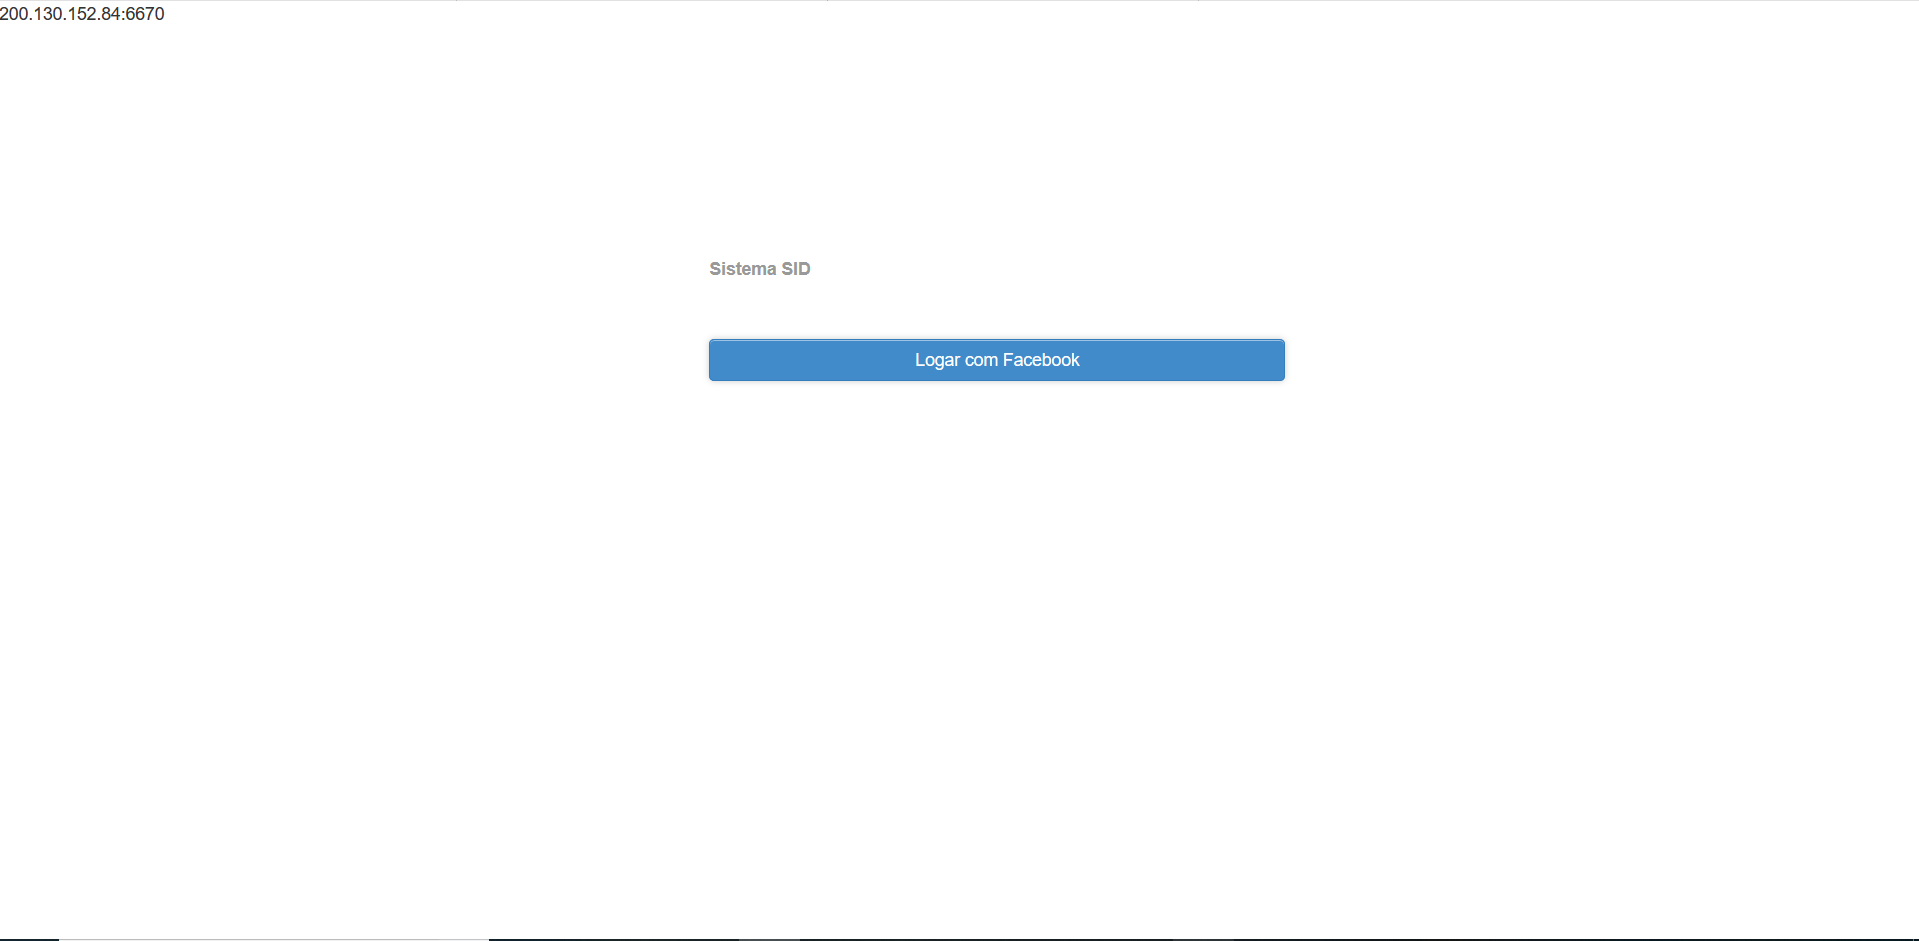
\includegraphics[width=\textwidth]{figuras/telalogar}
                \caption{Tela de login do Administrador}
            \end{figure}
        \item Campos\\
            Não se aplica.
        \item Comandos
            \begin{table}[H]
                \caption{Comandos da tela de logar}
                \resizebox{\textwidth}{!}{%
                \begin{tabular}{|c|c|c|c|c|}
                \hline
Nome & Descrição & Grupo & Requisitos de validade & Requisitos Diversos \\ \hline
Logar com Facebook & Usa a conta do Facebook do usuário para fazer login. & Todos & Autoriza se a conta estiver registrada no banco. & Deve possuir uma conta no Facebook. \\ \hline
                \end{tabular}%
                }
            \end{table}
    \end{itemize}
        
    \subsubsection{Interface do Administrador (Inserir)}
       \begin{itemize}
        \item Leiaute
            \begin{figure}[H]
                \centering
                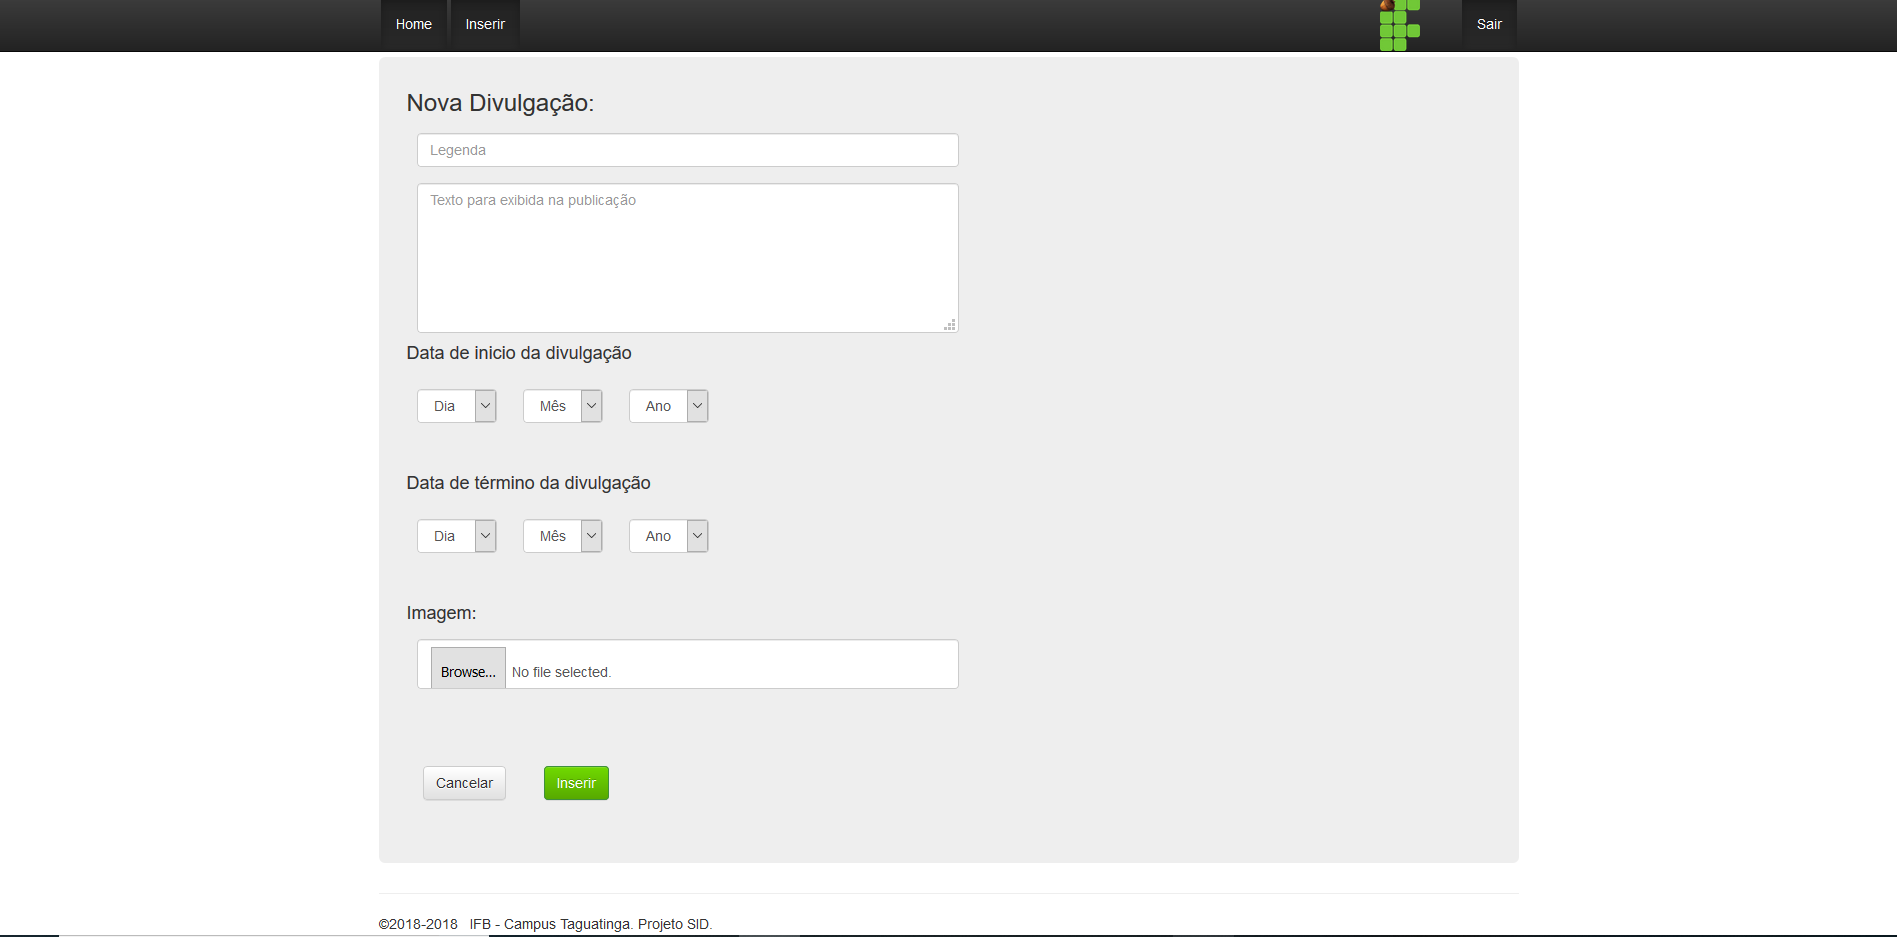
\includegraphics[width=\textwidth]{figuras/telainserir}
                \caption{Tela de inserção de novas publicações}
            \end{figure}
        
        \item Campos
        \begin{table}[H]
            \caption{Campos da tela de inserção}
            \resizebox{\textwidth}{!}{%
                \begin{tabular}{|c|c|c|c|c|c|}
                \hline
Nome & Descrição & Grupo & Requisitos de conteúdo & Requisitos de edição & Requisitos Diversos \\ \hline
Legenda & Legenda que irá ser apresentada no cliente. & Admin & Texto & -- & -- \\ \hline
Texto & Texto da publicação que será postada no Facebook. & Admin & Texto & -- & -- \\ \hline
Data de início & Data em que a publicação começará a ser exibida no cliente. & Admin & Inteiro selecionável entre as opções apresentadas & -- & -- \\ \hline
Data de Término & Data em que a publicação deixará de ser exibida no cliente. & Admin & Inteiro selecionável entre as opções apresentadas & -- & -- \\ \hline
Imagem & Imagem que irá ser apresentada na publicação do Facebook e no Cliente. & Admin & Arquivo do tipo imagem. & -- & A imagem deve ter o formato suportado pelo Facebook \\ \hline
                \end{tabular}%
            }
            \end{table}
        \item Comandos
            \begin{table}[H]
                \caption{Comandos da tela de inserção}
                \resizebox{\textwidth}{!}{%
                \begin{tabular}{|c|c|c|c|c|}
                \hline
Nome & Descrição & Grupo & Requisitos de validade & Requisitos Diversos \\ \hline
Inserir & Insere no banco e no Facebook as informações descritas nos campos. & admin & Todos os campos devem estar preenchidos. & -- \\ \hline
Cancelar & Cancela a inserção dos dados e retorna para a lista de publicações criadas. & admin & -- & -- \\ \hline
                \end{tabular}%
                }
            \end{table}
    \end{itemize}
        
    \subsubsection{Interface do Administrador (Listar)}
        \begin{itemize}
        \item Leiaute
            \begin{figure}[H]
                \centering
                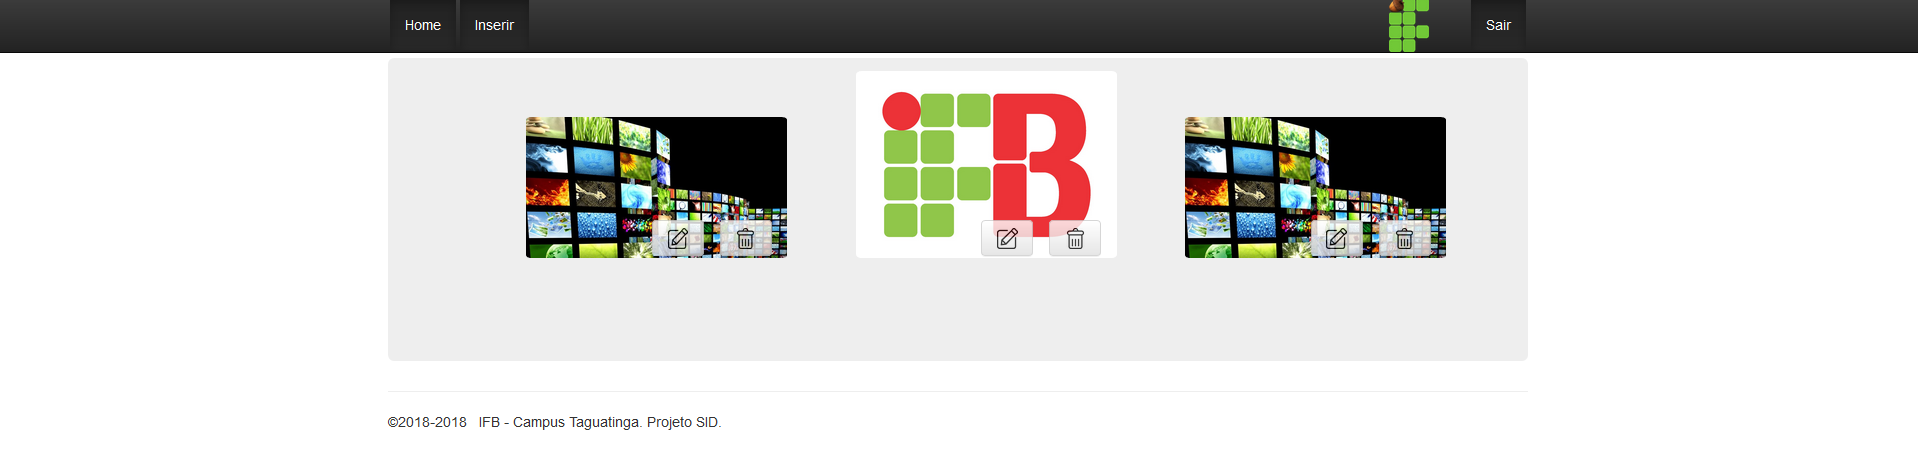
\includegraphics[width=\textwidth]{figuras/telalistar}
                \caption{Tela de listagem das publicações}
            \end{figure}
        \item Campos\\
            Não se aplica.
        \item Comandos
                \begin{table}[H]
                \caption{Comandos da tela de listagem}
                \resizebox{\textwidth}{!}{%
                \begin{tabular}{|c|c|c|c|c|}
                \hline
Nome & Descrição & Grupo & Requisitos de validade & Requisitos Diversos \\ \hline
Detalhar & Clicar sobre a imagem retorna a páginacom  detalhes da publicação. & admin & -- & -- \\ \hline
Editar & O ícone de editar, retorna pagina de edição. & admin & -- & -- \\ \hline
Deletar & O ícone de excluir, exclui a publicação do banco e do Cliente. & admin & -- & -- \\ \hline
                \end{tabular}%
                }
            \end{table}
    \end{itemize}
        
    \subsubsection{Interface do Administrador (Editar)}
        \begin{itemize}
        \item Leiaute
            \begin{figure}[H]
                \centering
                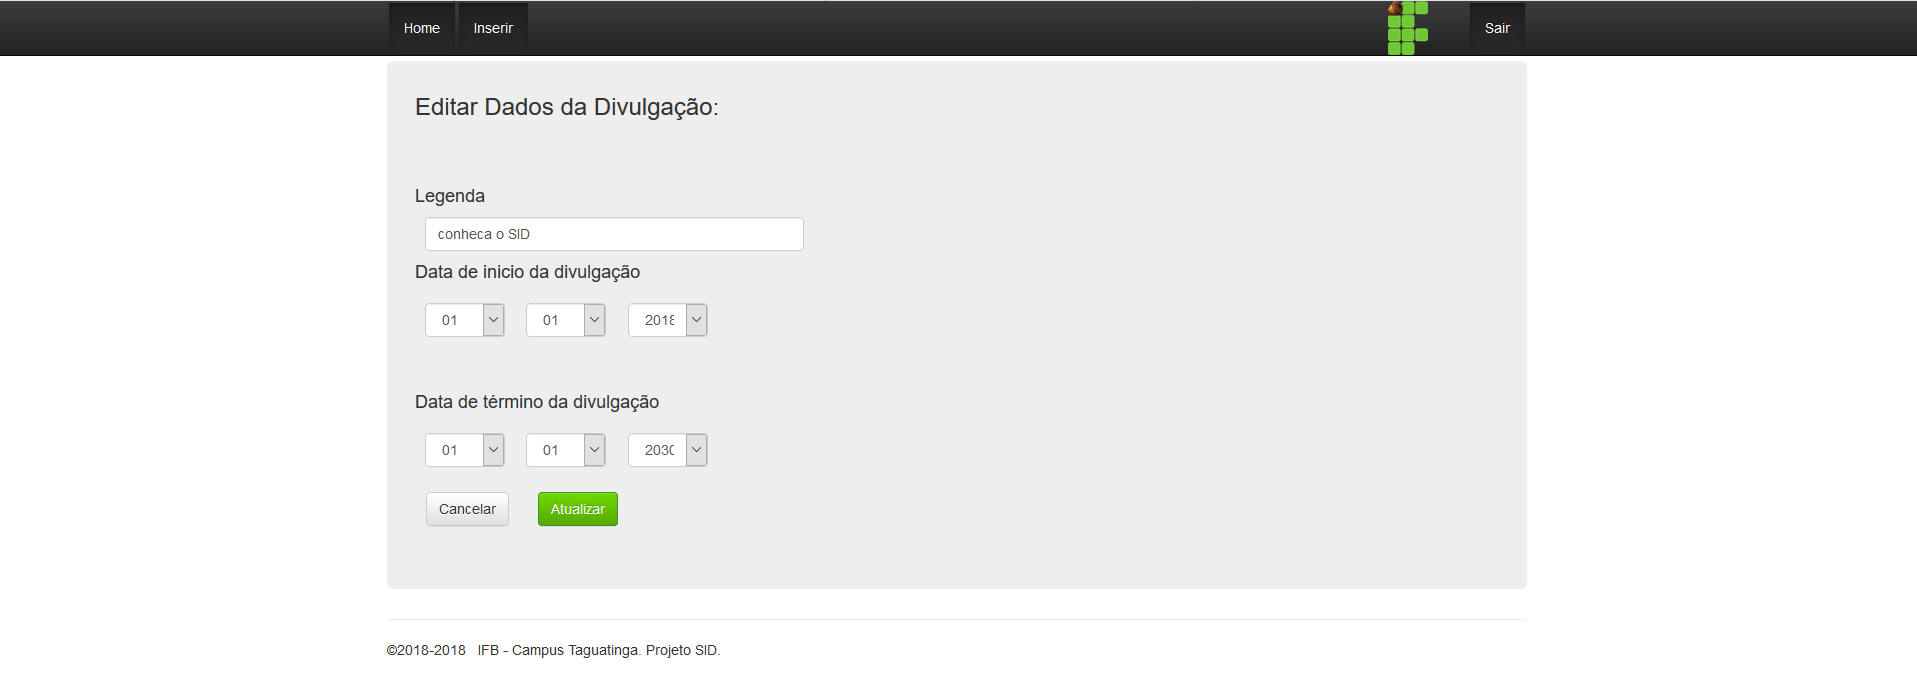
\includegraphics[width=\textwidth]{figuras/telaeditar}
                \caption{Tela de edição das publicações}
            \end{figure}
        \item Campos
\begin{table}[H]
            \caption{Campos da tela de edição}
            \resizebox{\textwidth}{!}{%
                \begin{tabular}{|c|c|c|c|c|c|}
                \hline
Nome & Descrição & Grupo & Requisitos de conteúdo & Requisitos de edição & Requisitos Diversos \\ \hline
Legenda & Legenda que irá ser apresentada no cliente. & Admin & Texto & -- & -- \\ \hline
Data de início & Data em que a publicação começará a ser exibida no cliente. & Admin & Inteiro selecionável entre as opções apresentadas & -- & -- \\ \hline
Data de Término & Data em que a publicação deixará de ser exibida no cliente. & Admin & Inteiro selecionável entre as opções apresentadas & -- & -- \\ \hline
                \end{tabular}%
            }
            \end{table}
        \item Comandos
            \begin{table}[H]
                \caption{Comandos da tela de edição}
                \resizebox{\textwidth}{!}{%
                \begin{tabular}{|c|c|c|c|c|}
                \hline
Nome & Descrição & Grupo & Requisitos de validade & Requisitos Diversos \\ \hline
Atualizar & Realiza a atualização no banco com os novos dados & admin & Todos os campos devem estar preenchidos & -- \\ \hline
Cancelar & Cancela as alterações e retorna a página de listagem & admin & -- & -- \\ \hline
                \end{tabular}%
                }
            \end{table}
    \end{itemize}
        
    \subsubsection{Interface do Administrador (Detalhar)}
        \begin{itemize}
        \item Leiaute
            \begin{figure}[H]
                \centering
                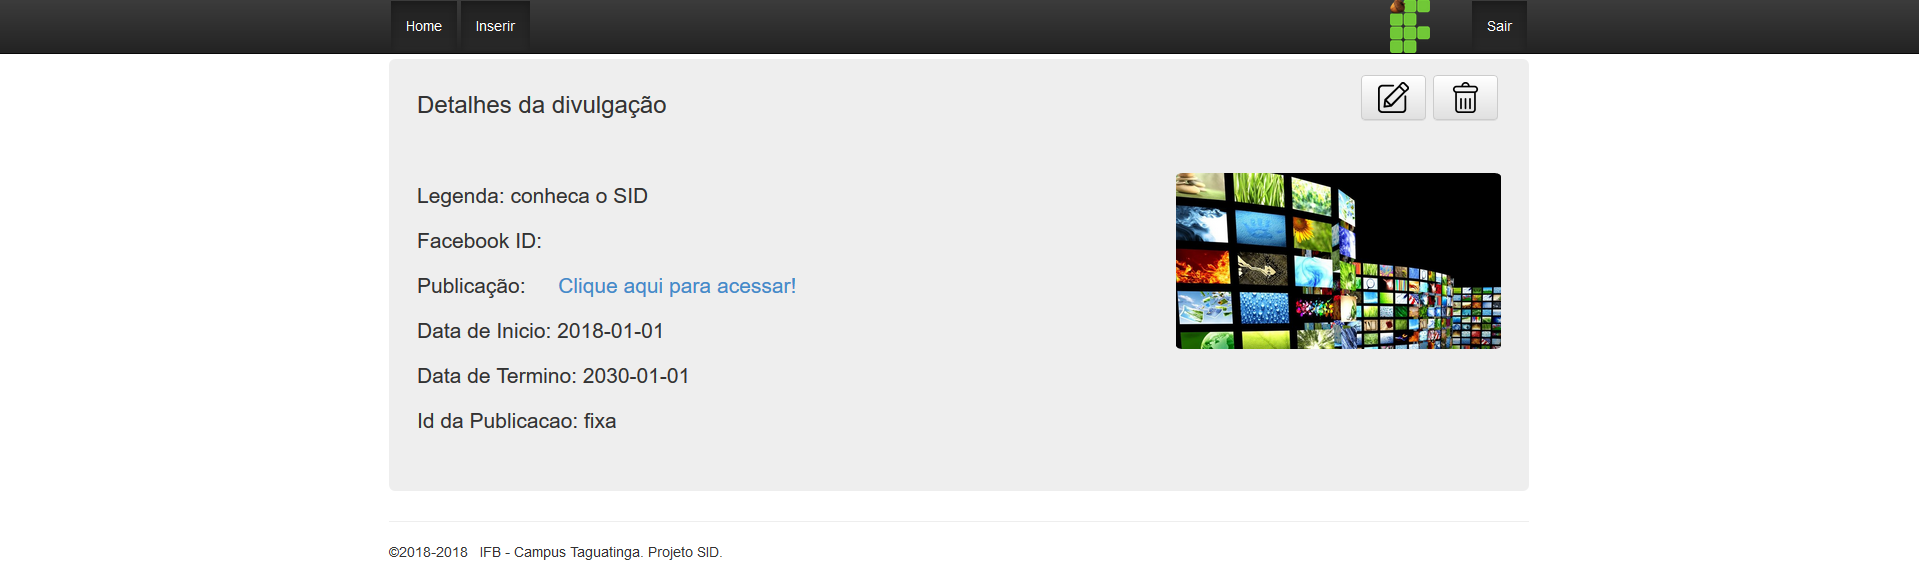
\includegraphics[width=\textwidth]{figuras/teladetalhar}
                \caption{Tela de detalhamento das publicações}
            \end{figure}
        \item Campos\\
            Não se aplica.
        \item Comandos
            \begin{table}[H]
                \caption{Comandos da tela de detalhamento}
                \resizebox{\textwidth}{!}{%
                \begin{tabular}{|c|c|c|c|c|}
                \hline
Nome & Descrição & Grupo & Requisitos de validade & Requisitos Diversos \\ \hline
Clique Aqui & Acessa aolink da publicação no Facebook. & admin & -- & -- \\ \hline
Editar & O ícone de editar, retorna pagina de edição. & admin & -- & -- \\ \hline
Deletar & O ícone de excluir, exclui a publicação do banco e do Cliente. & admin & -- & -- \\ \hline
                \end{tabular}%
                }
            \end{table}
    \end{itemize}
        
    \subsubsection{Interface Cliente}
        \begin{itemize}
        \item Leiaute
            \begin{figure}[H]
                \centering
                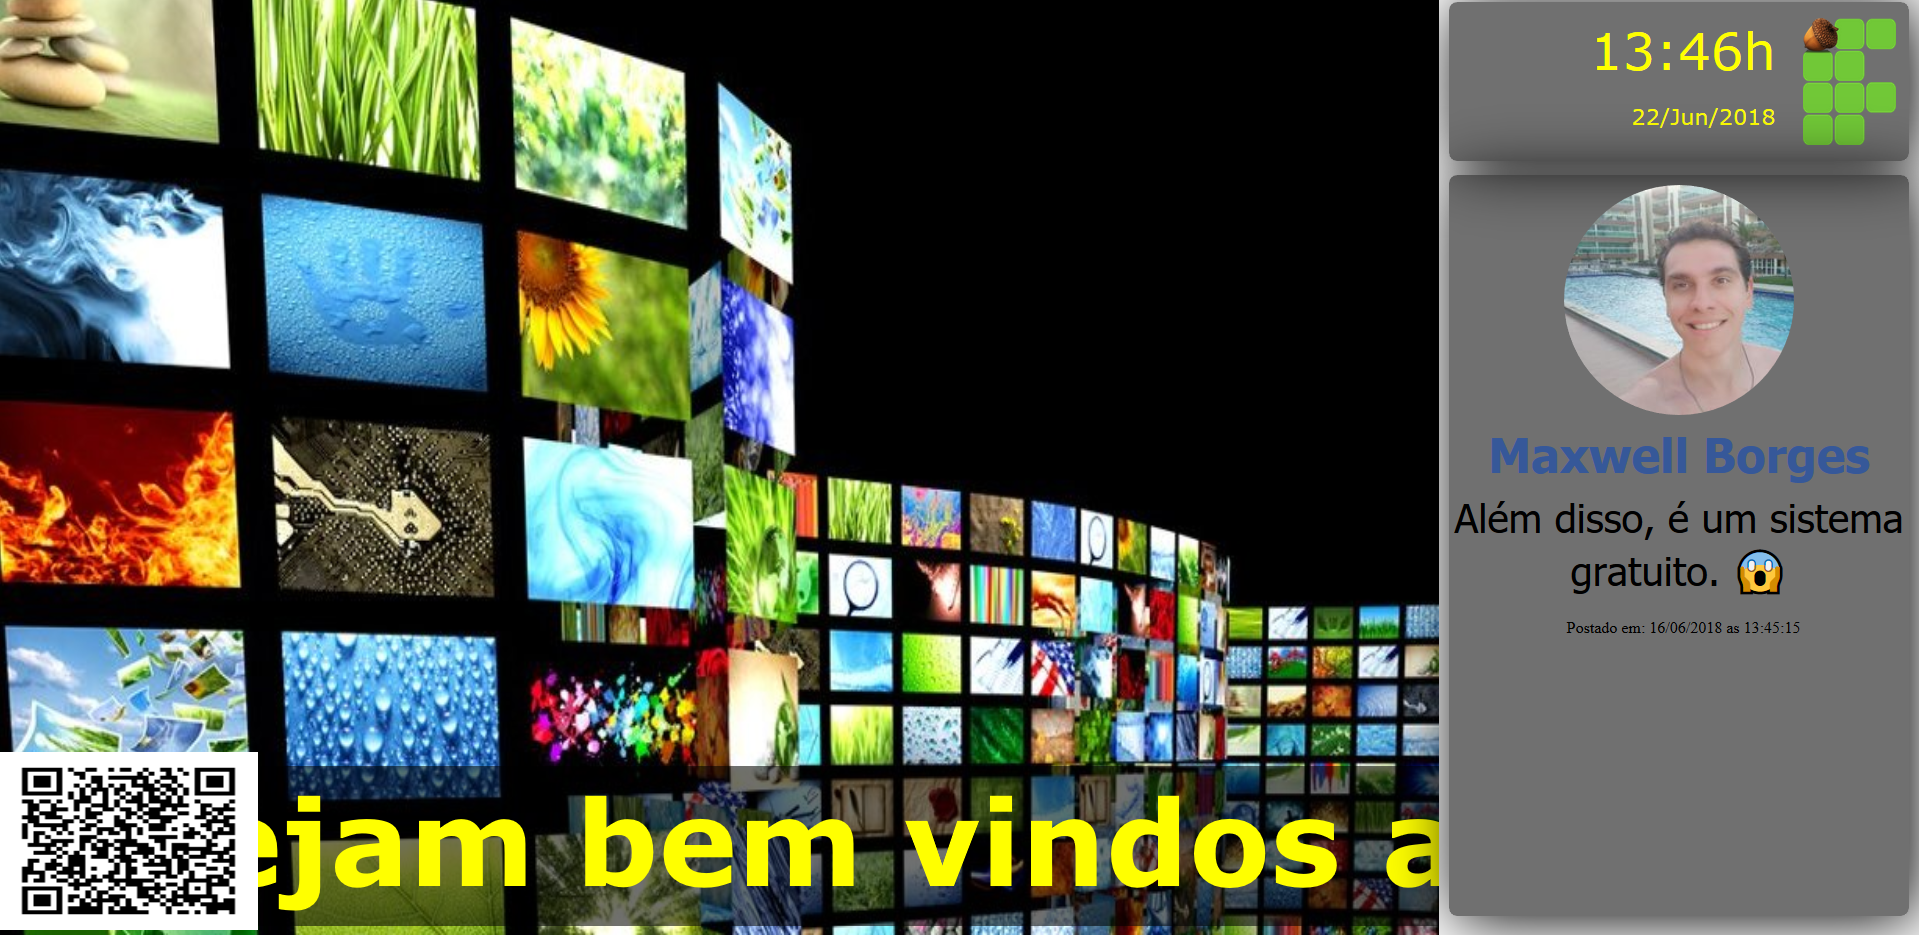
\includegraphics[width=\textwidth]{figuras/telacliente}
                \caption{Tela do cliente}
            \end{figure}
        \item Campos\\
            Não se aplica.
        \item Comandos\\
            Não se aplica.
        \end{itemize}
\clearpage

\section{Diagramas}
\label{diagramas}
\subsection{Diagramas de casos de uso}
\begin{figure}[H]
    \centering
    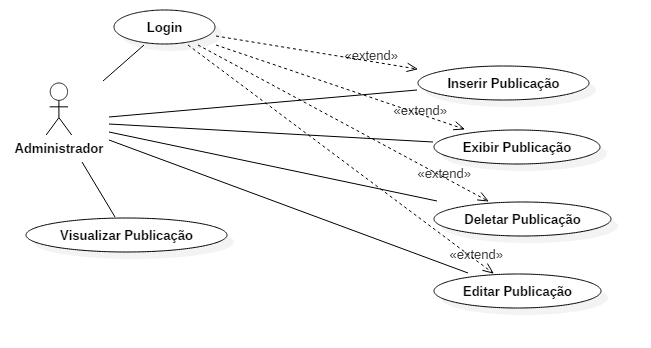
\includegraphics[width=\textwidth]{figuras/casosDeUsoADM}
    \caption{Diagrama de casos de uso do módulo administrador}
\end{figure}

\begin{figure}[H]
    \centering
    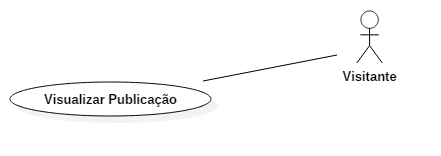
\includegraphics[width=\textwidth]{figuras/CasosDeUsoCliente}
    \caption{Diagrama de casos de uso do módulo cliente}
\end{figure}

\begin{figure}
    \centering
    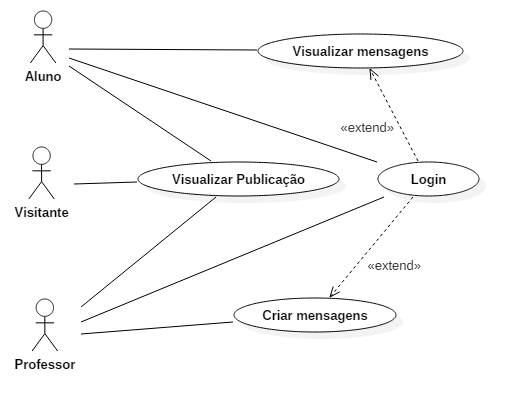
\includegraphics[width=\textwidth]{figuras/CasosDeUsoMobile}
    \caption{Diagrama de casos de uso do aplicativo móvel}
\end{figure}

\subsection{Diagramas de classe}
\begin{figure}[H]
    \centering
    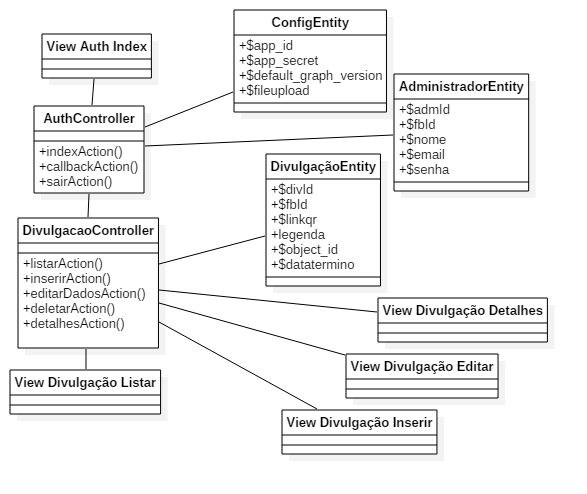
\includegraphics[width=\textwidth]{figuras/diagramaclasseADM}
    \caption{Diagrama de classes do módulo administrador}
\end{figure}

\begin{figure}[H]
    \centering
    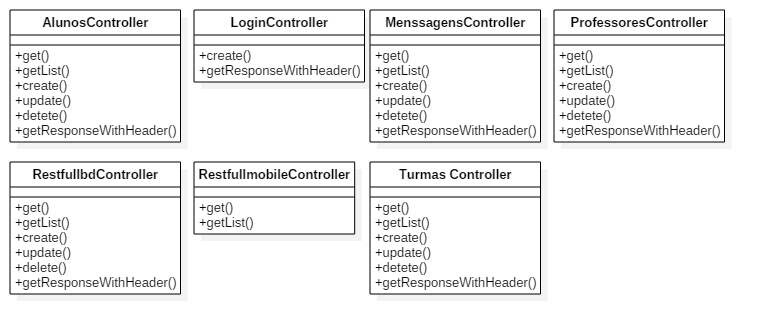
\includegraphics[width=\textwidth]{figuras/diagramaclasseAPI}
    \caption{Diagrama de classes do submódulo API}
\end{figure}

\begin{figure}[H]
    \centering
    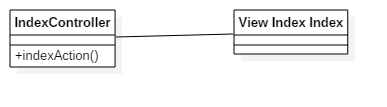
\includegraphics[width=\textwidth]{figuras/diagramaclasseCLIENTE}
    \caption{Diagrama de classes do módulo Cliente}
\end{figure}

\subsection{Diagramas entidade--relacionamento}
\begin{figure}[H]
    \centering
    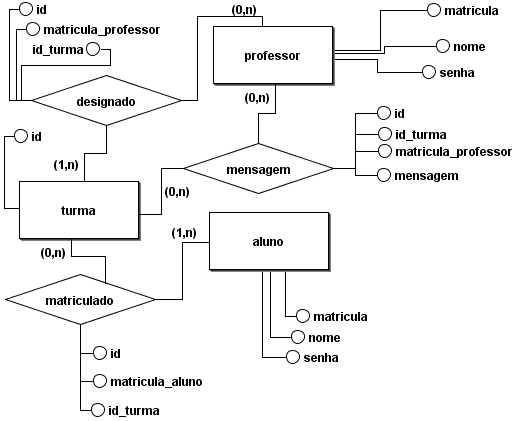
\includegraphics[width=\textwidth]{figuras/entidaderelacionamentomobile}
    \caption{Diagrama entidade--relacionamento do aplicativo móvel (API fictícia)}
\end{figure}

\begin{figure}[H]
    \centering
    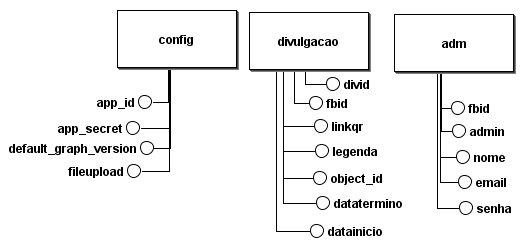
\includegraphics[width=\textwidth]{figuras/entidaderelacionamento}
    \caption{Diagrama entidade--relacionamento do \textit{web}}
\end{figure}

\subsection{Diagramas de sequência}
\begin{figure}[H]
    \centering
    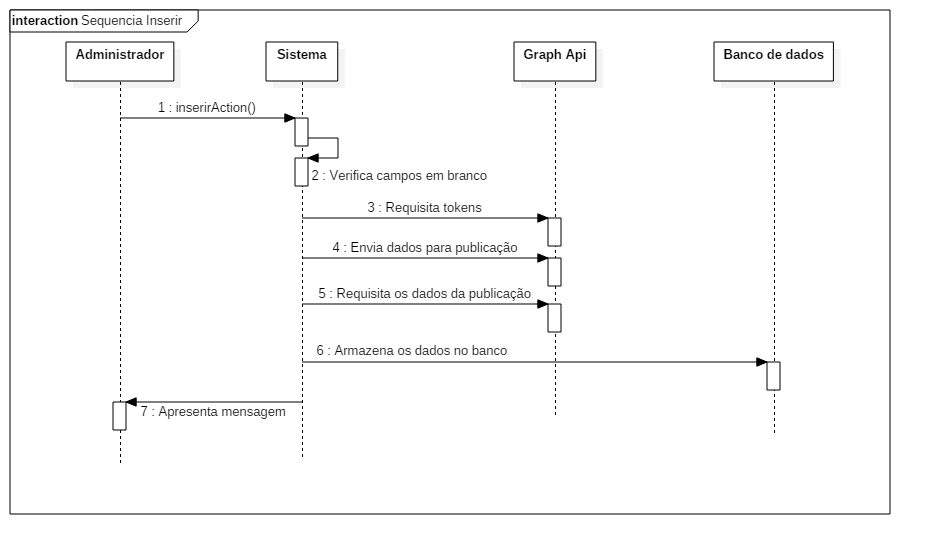
\includegraphics[width=\textwidth]{figuras/sequenciainserir}
    \caption{Diagrama de sequência para inserir}
\end{figure}

\begin{figure}[H]
    \centering
    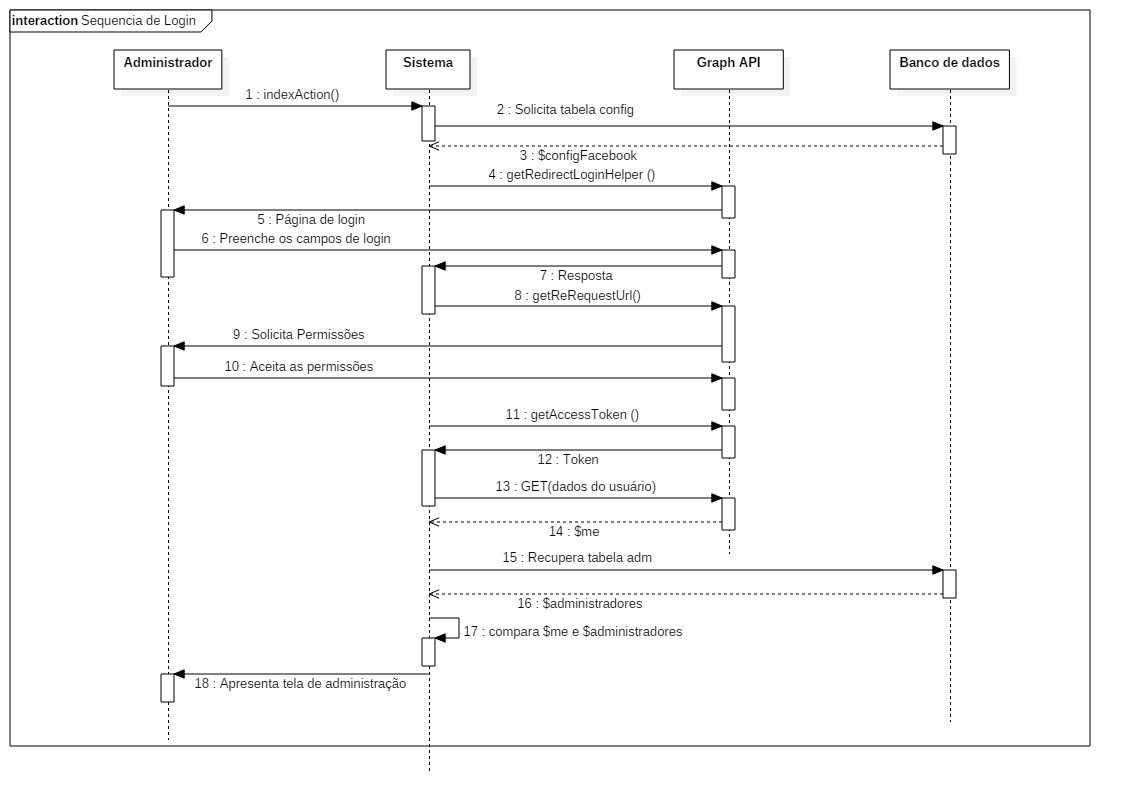
\includegraphics[width=\textwidth]{figuras/sequencialogin}
    \caption{Diagrama de sequência para login}
\end{figure}

\begin{figure}[H]
    \centering
    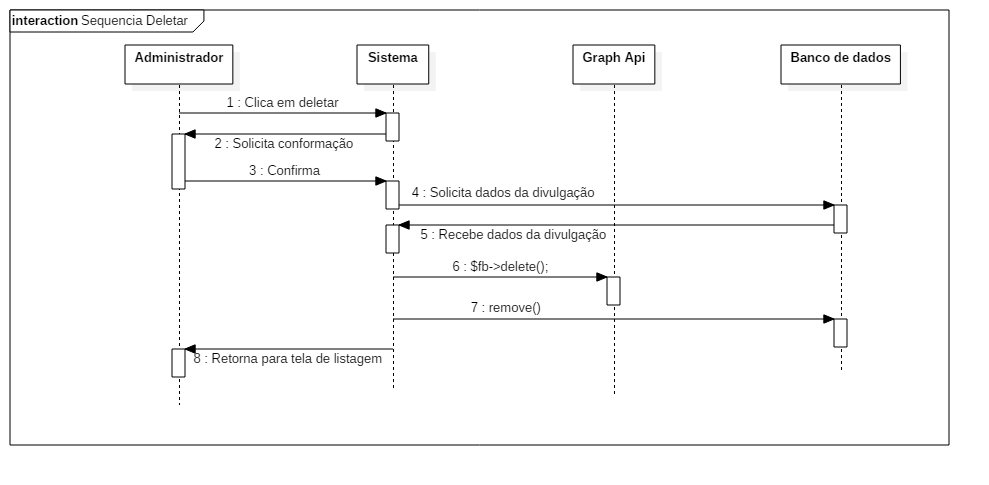
\includegraphics[width=\textwidth]{figuras/sequenciaDeletar}
    \caption{Diagrama de sequência para deletar}
\end{figure}

\begin{figure}[H]
    \centering
    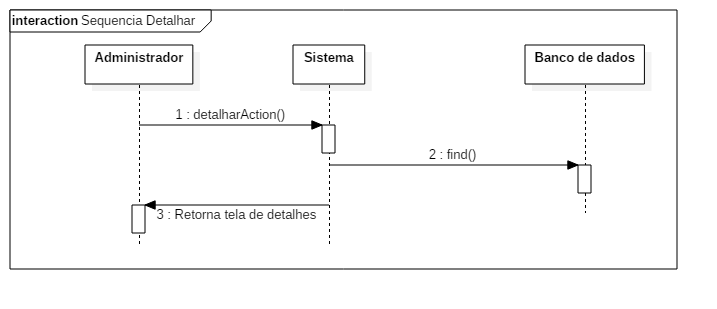
\includegraphics[width=\textwidth]{figuras/sequenciaDetalhar}
    \caption{Diagrama de sequência para detalhar}
\end{figure}

\begin{figure}[H]
    \centering
    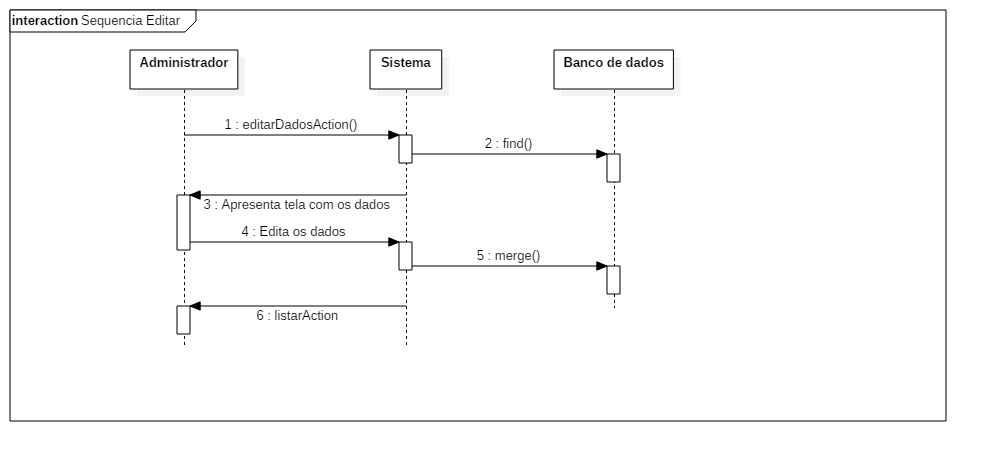
\includegraphics[width=\textwidth]{figuras/sequenciaEditar}
    \caption{Diagrama de sequência para editar}
\end{figure}

\begin{figure}[H]
    \centering
    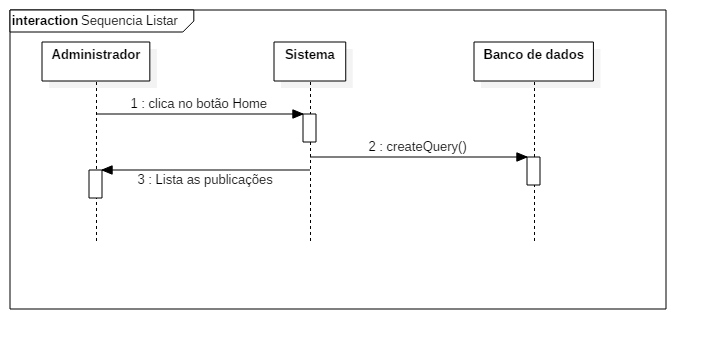
\includegraphics[width=\textwidth]{figuras/sequenciaListar}
    \caption{Diagrama de sequência para listar}
\end{figure}
\clearpage

\section{Artefatos}
\label{artefatos}
\begin{table}[H]
\fontsize{8}{12}\selectfont
\caption{Requisitos de usuário}
\resizebox{\textwidth}{!}{%
\begin{tabular}{p{0.7cm}p{8cm}}
{[}RU01{]} & O sistema deverá permitir login dos administradores através do Facebook ou usando e--mail e senha do usuário cadastrados, autorizando que acessem ao sistema e nele realize as funções permitidas. \\
{[}RU02{]} & O sistema deverá permitir que o usuário devidamente cadastrado consiga criar publicações. \\
{[}RU03{]} & O sistema deverá permitir que o usuário devidamente cadastrado consiga editar as publicações que foram criadas. \\
{[}RU04{]} & O sistema deverá permitir que o usuário devidamente cadastrado consiga excluir uma ou mais publicações criadas. \\
{[}RU05{]} & O sistema deverá confirmar se o usuário deseja excluir uma publicação. \\
{[}RU06{]} & O sistema deverá listar todas as publicações criadas. \\
{[}RU07{]} & O sistema deverá armazenar todas as informações que forem inseridas para que possam serem feitas as edições, listagens e exclusões. \\
{[}RU08{]} & O sistema deverá possuir uma página de acesso público. \\
{[}RU09{]} & O sistema deverá apresentar apenas as publicações e comentários autorizados. \\
{[}RU10{]} & O sistema deverá possuir internet conectada. \\
{[}RU11{]} & O sistema deverá funcionar nos navegadores de internet dos sistemas operacionais Linux, Windows.
\end{tabular}%
}
\end{table}

\begin{figure}
    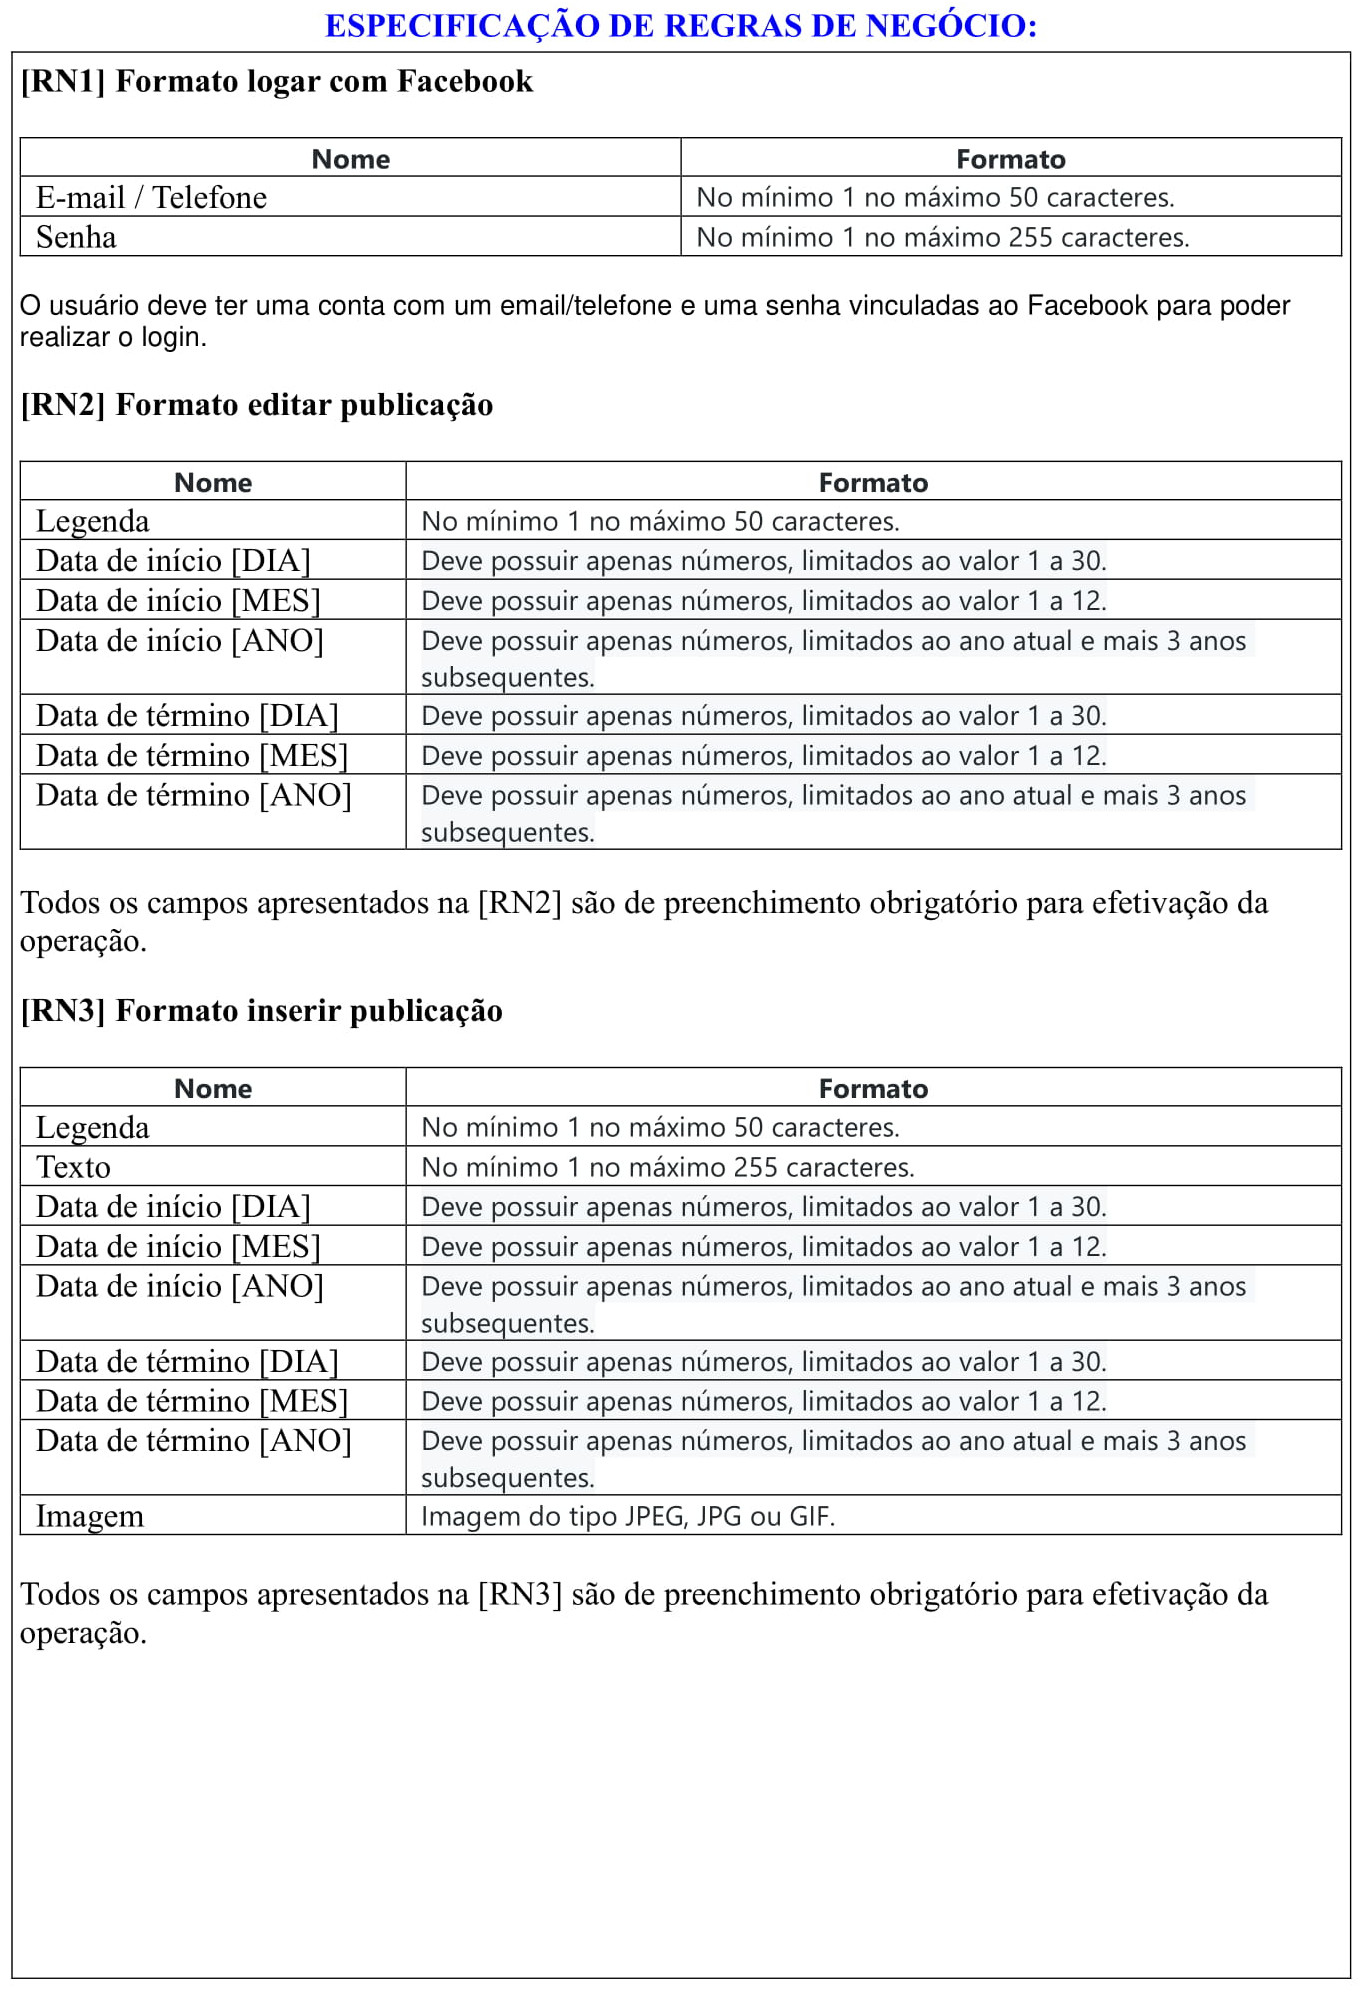
\includegraphics[width=\textwidth]{documentacao/ModeloArtefatos-01.jpg}
\end{figure}

\begin{figure}
    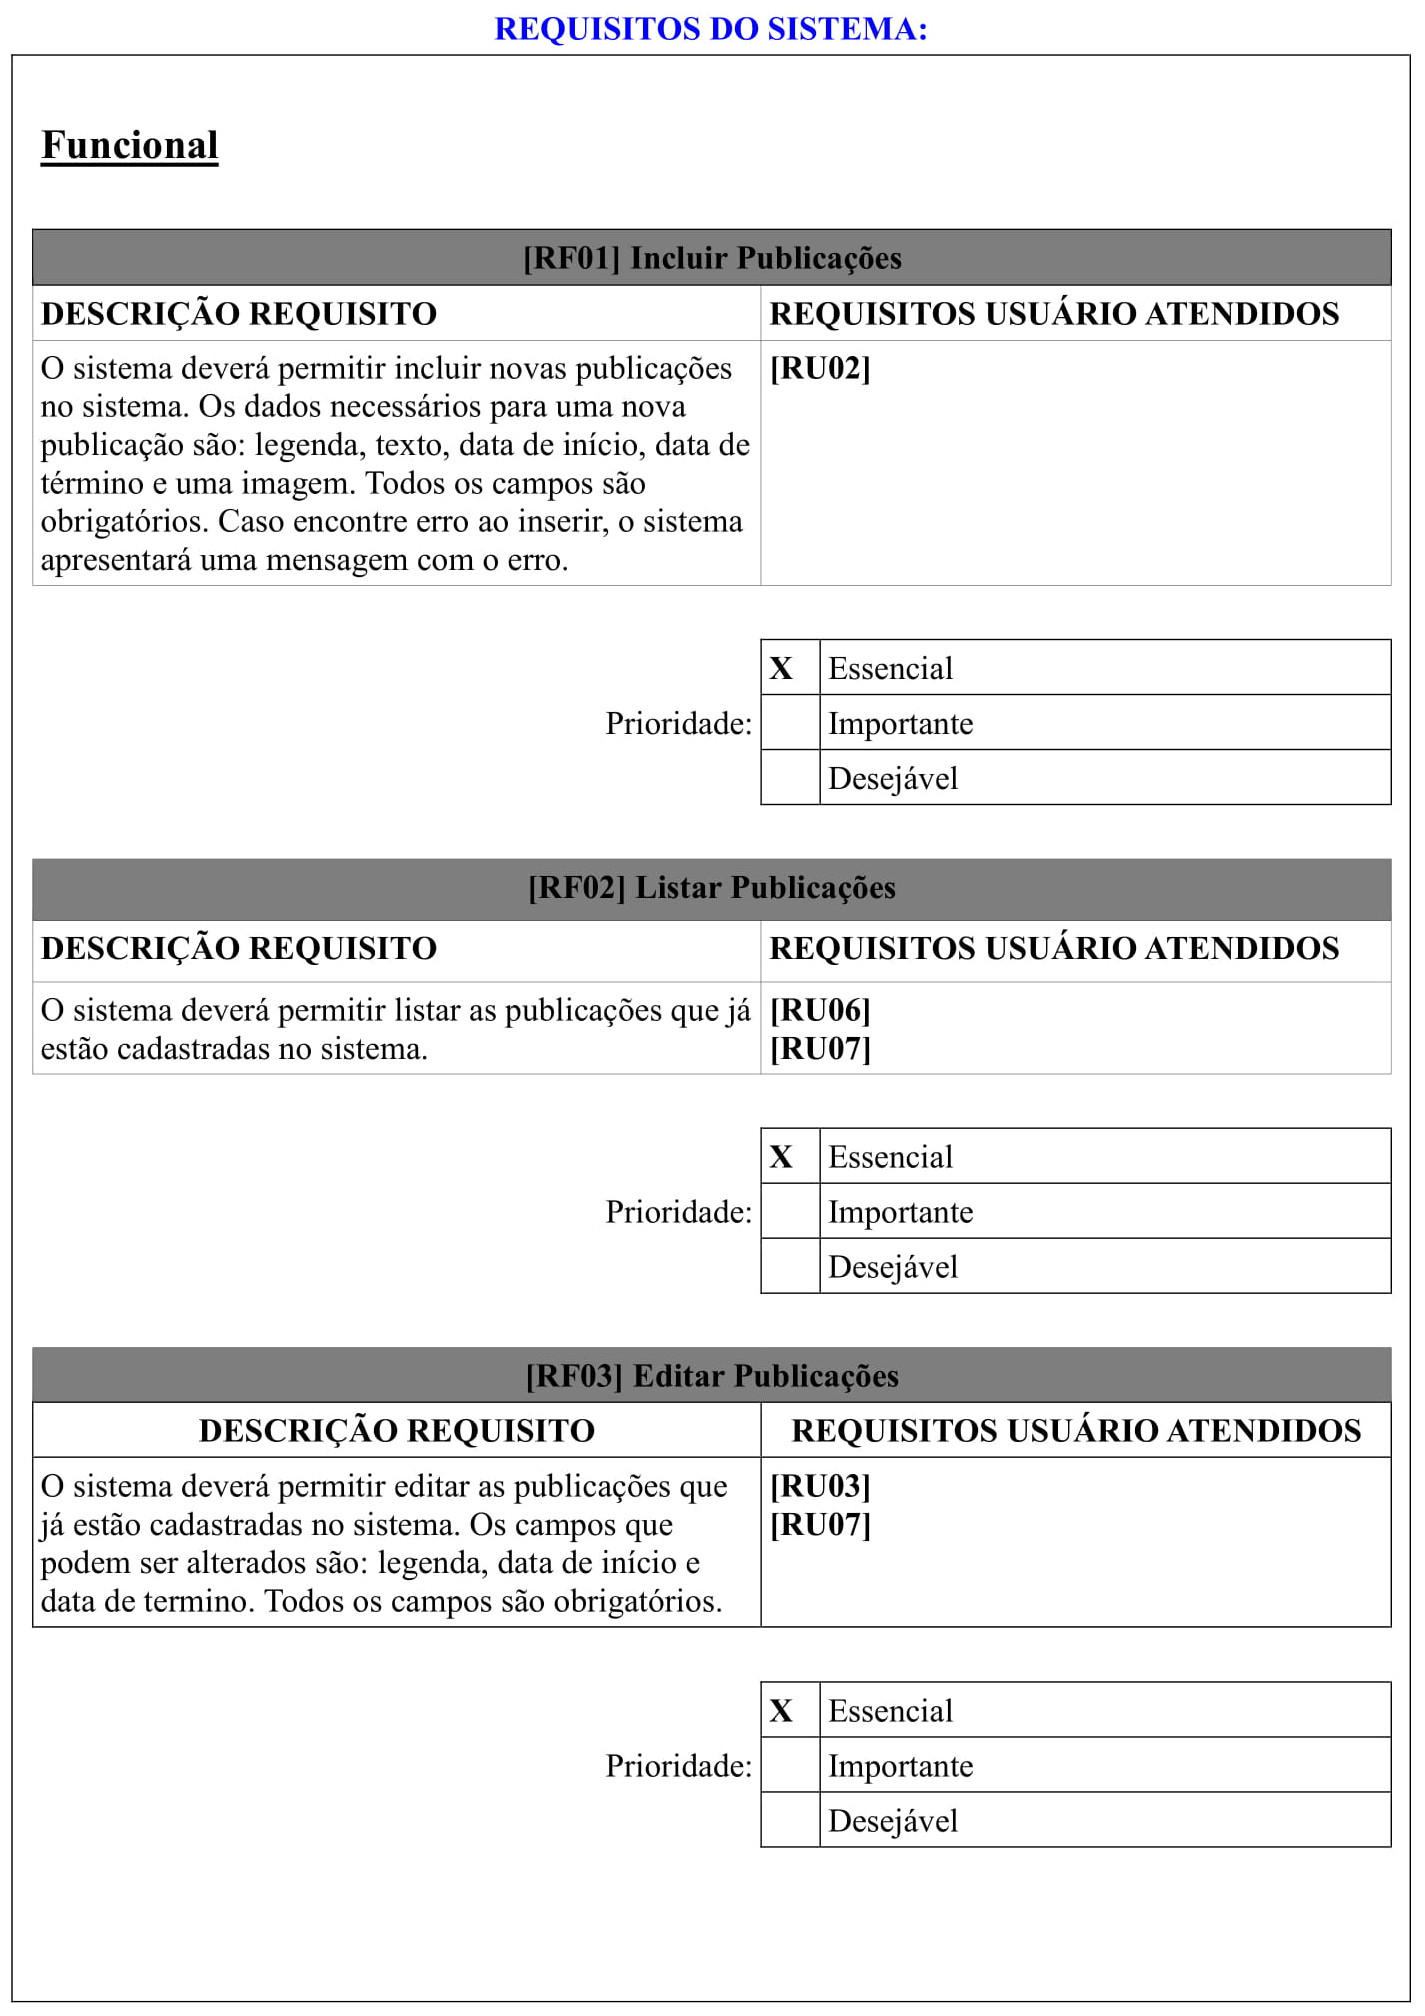
\includegraphics[width=\textwidth]{documentacao/ModeloArtefatos-02.jpg}
\end{figure}

\begin{figure}
    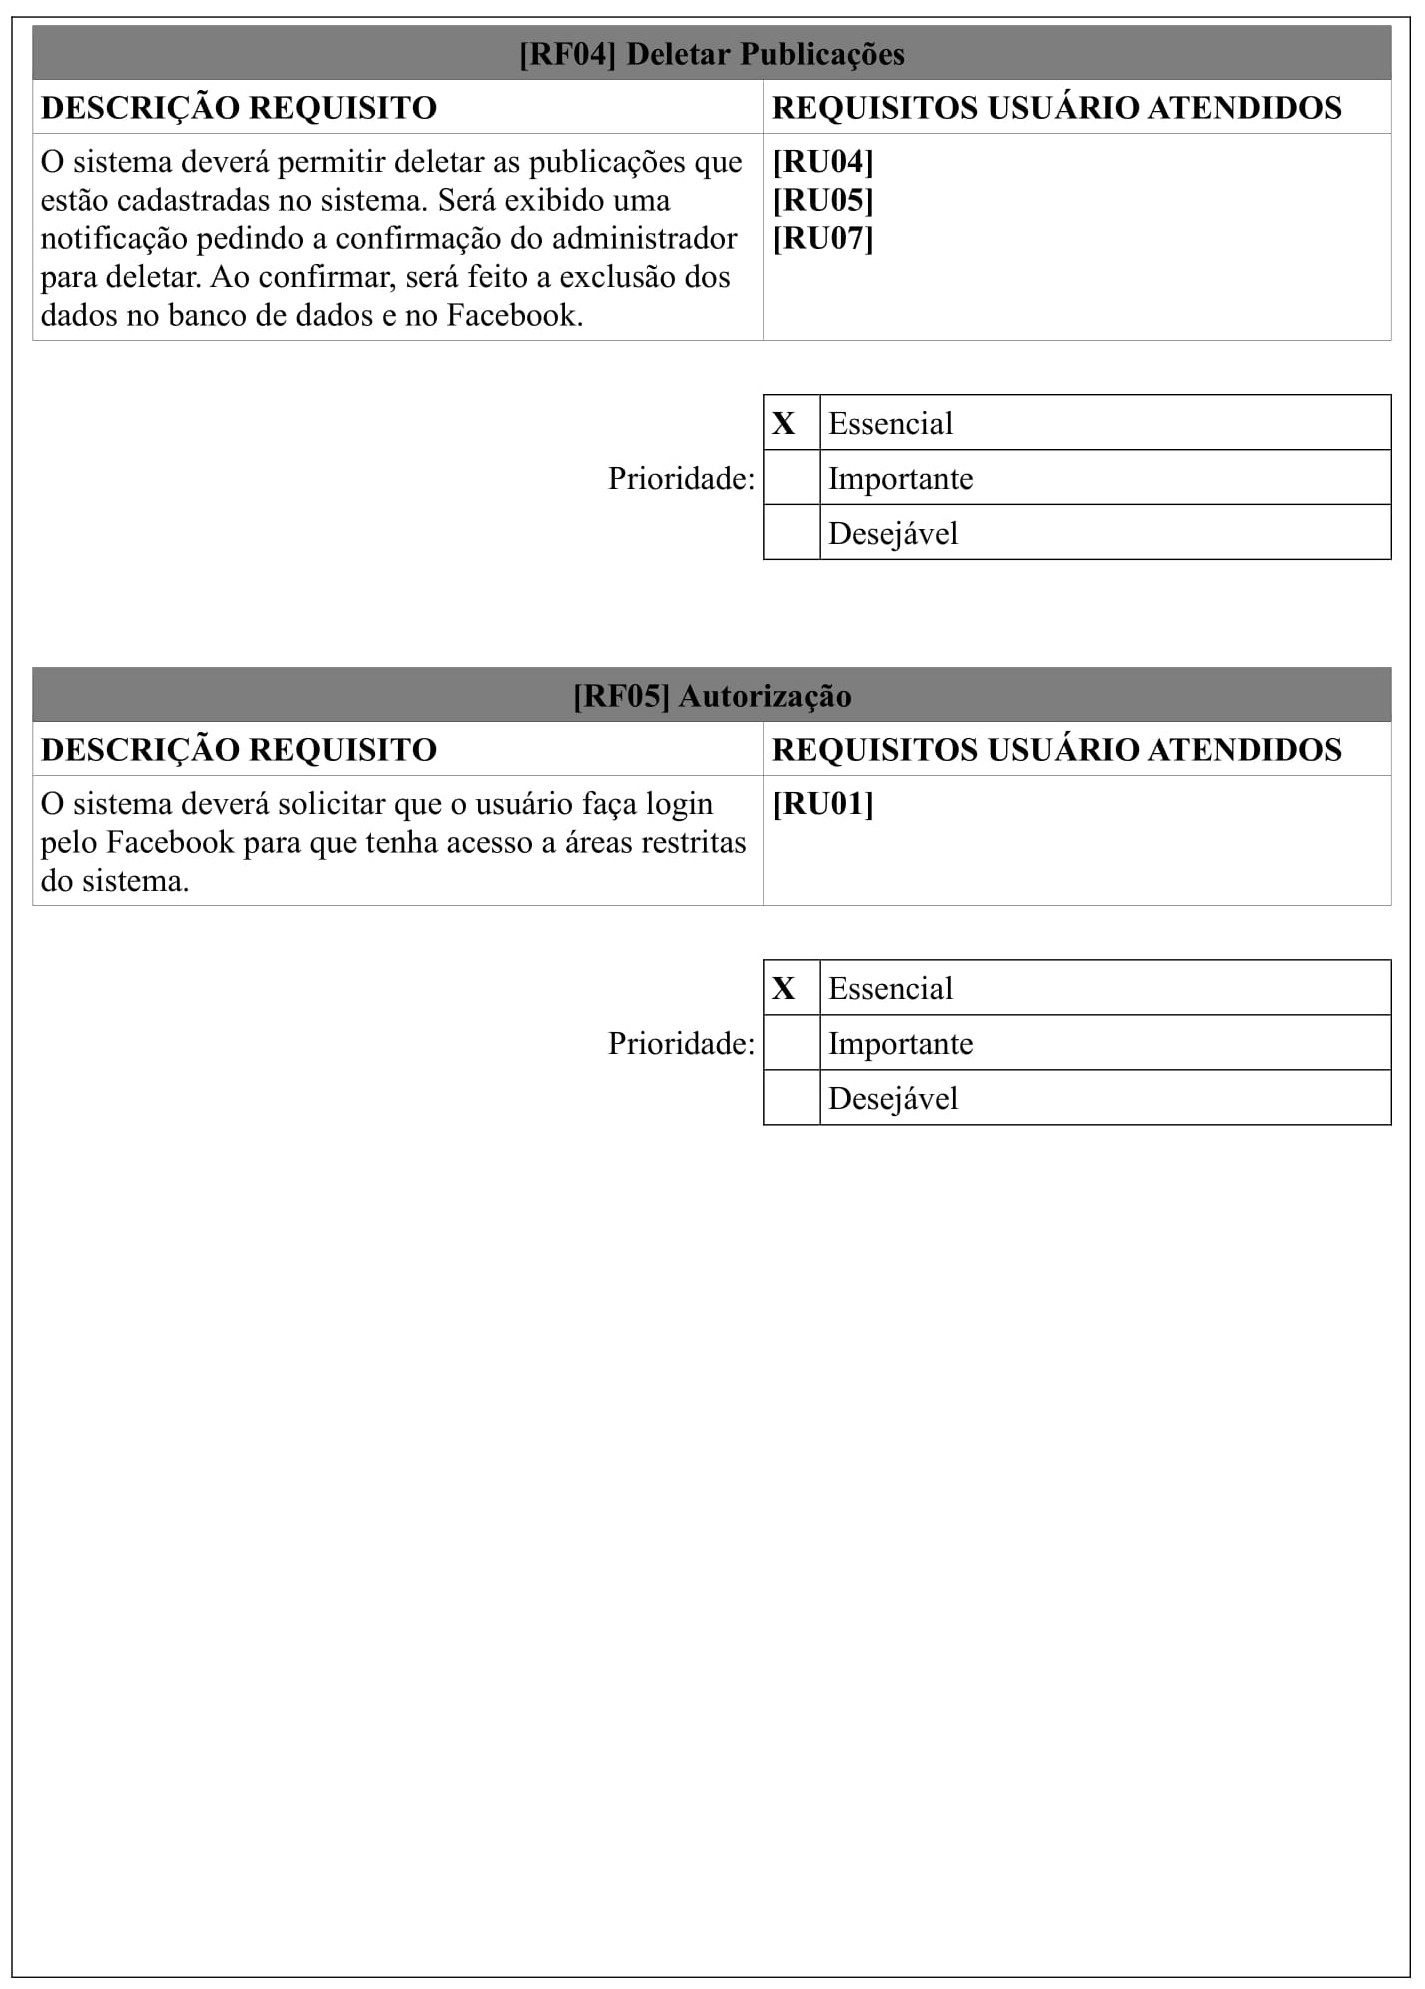
\includegraphics[width=\textwidth]{documentacao/ModeloArtefatos-03.jpg}
\end{figure}

\begin{figure}
    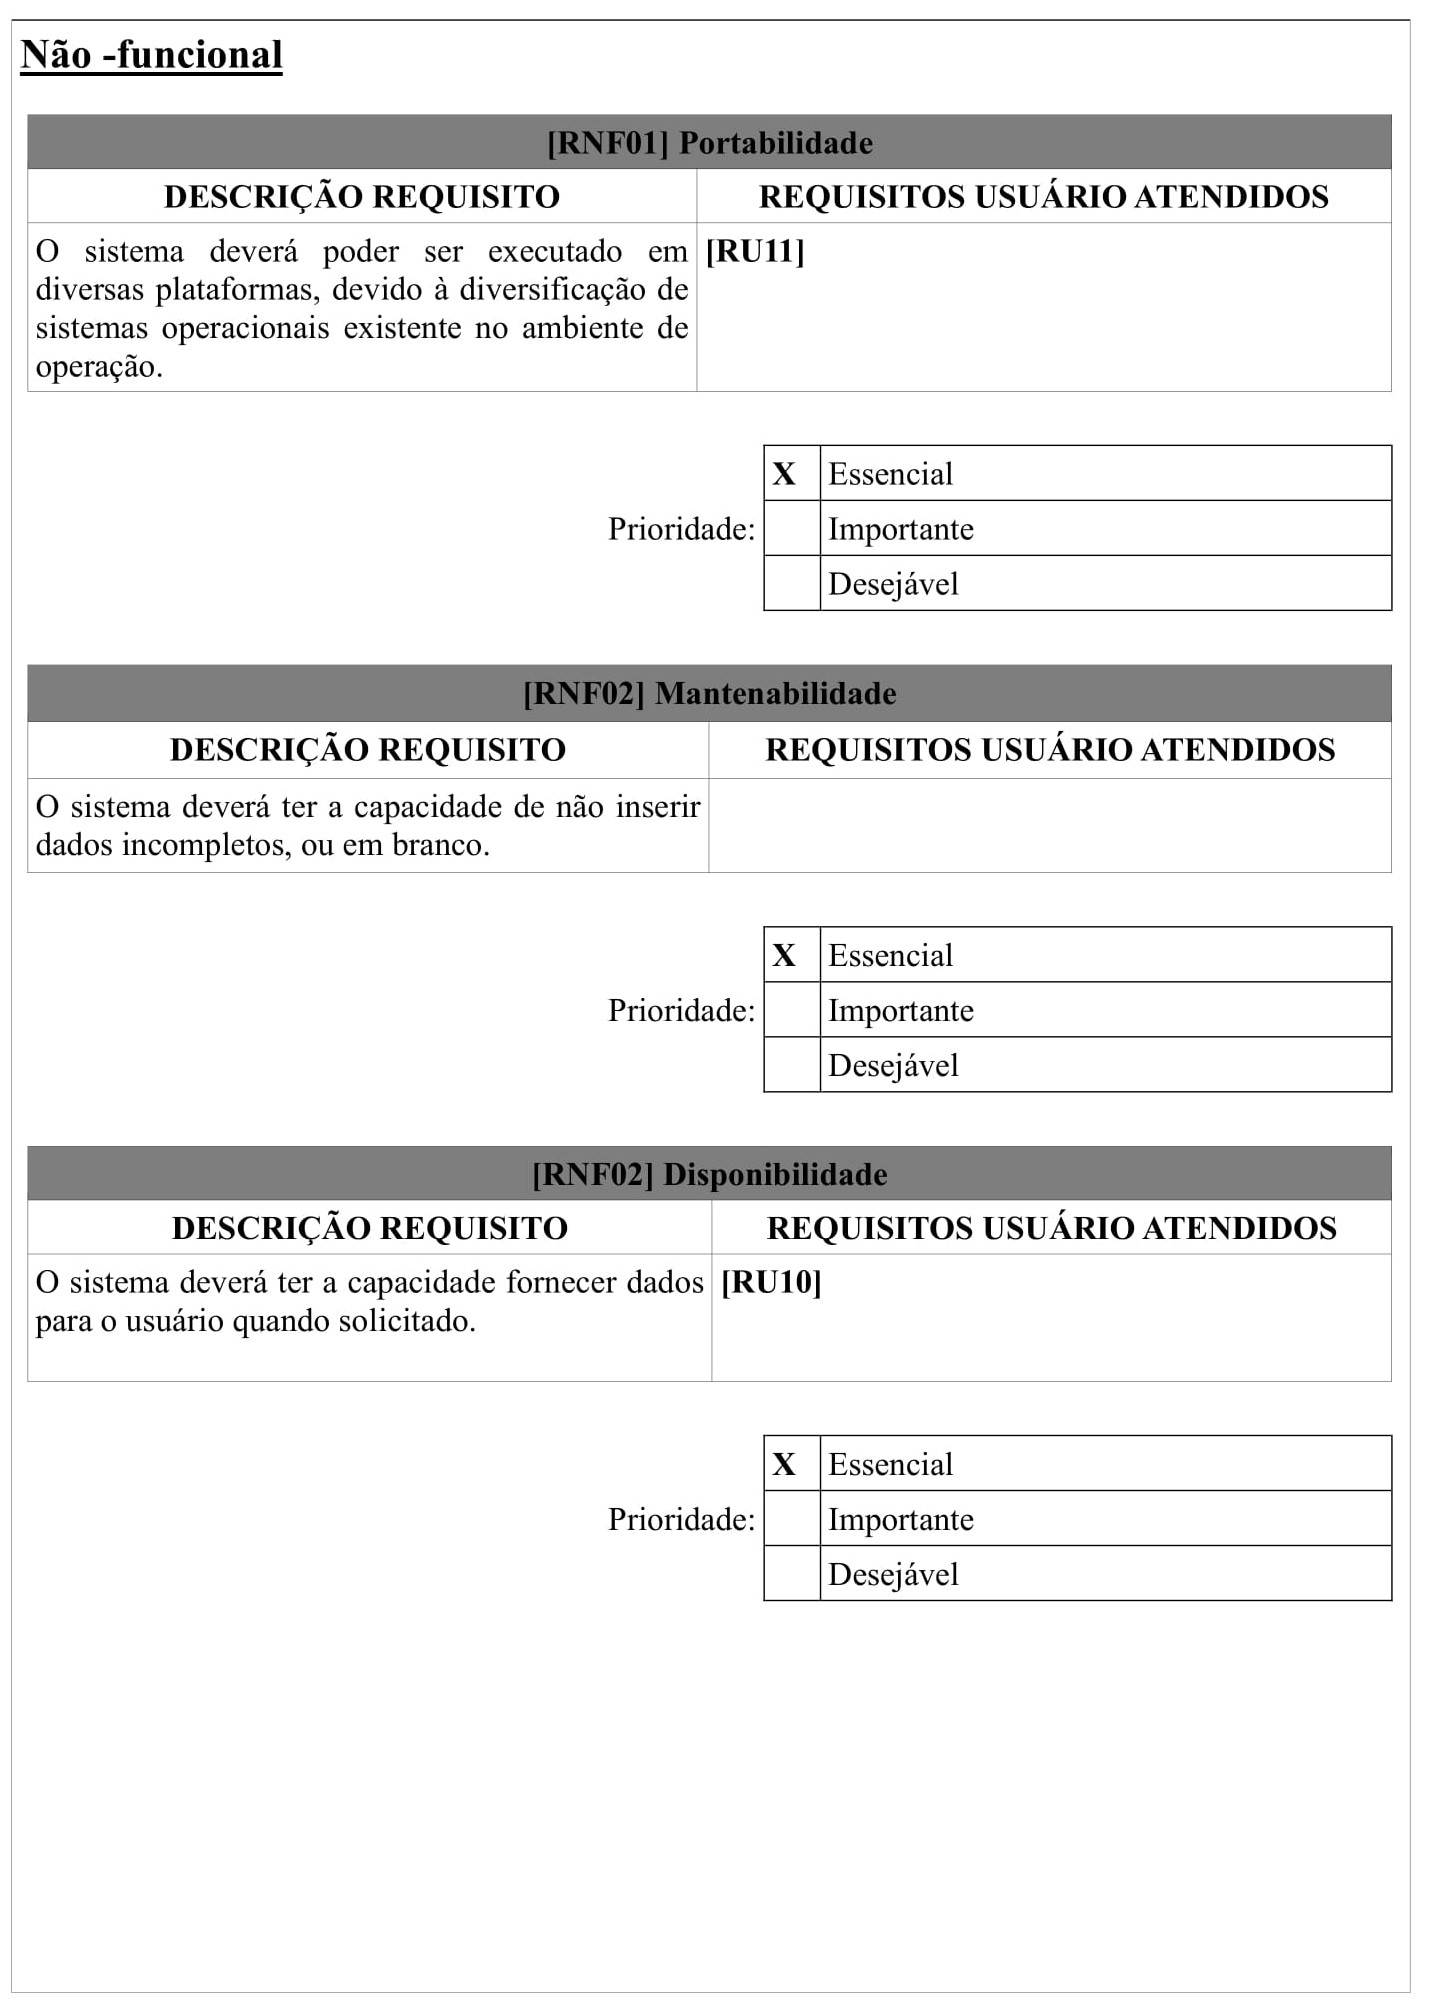
\includegraphics[width=\textwidth]{documentacao/ModeloArtefatos-04.jpg}
\end{figure}

\begin{figure}
    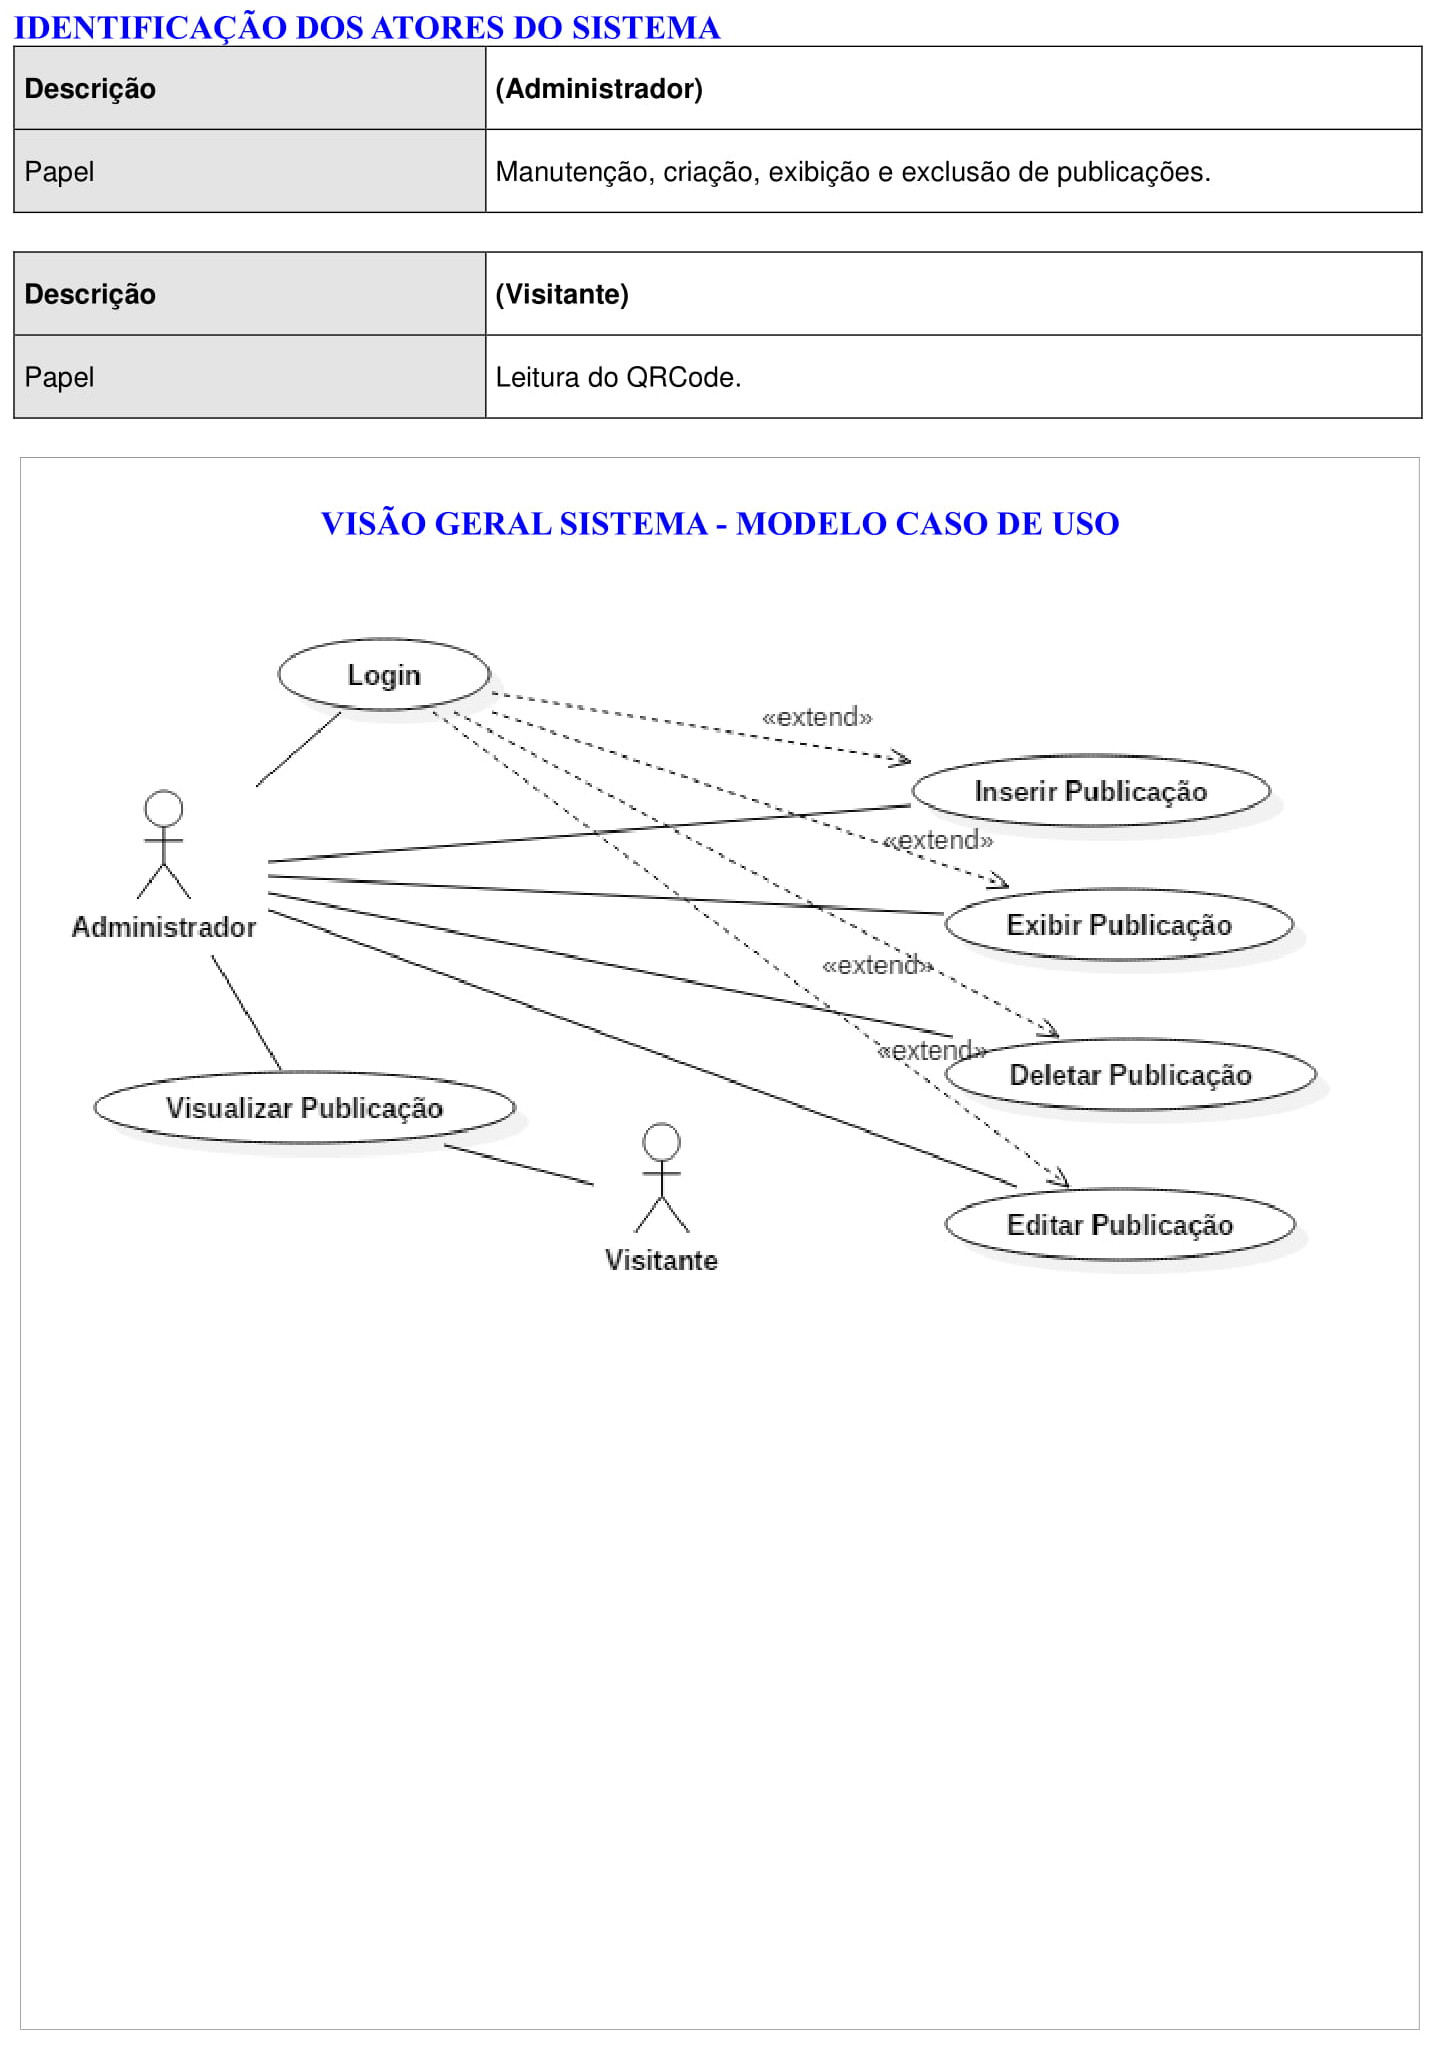
\includegraphics[width=\textwidth]{documentacao/ModeloArtefatos-05.jpg}
\end{figure}

\begin{figure}
    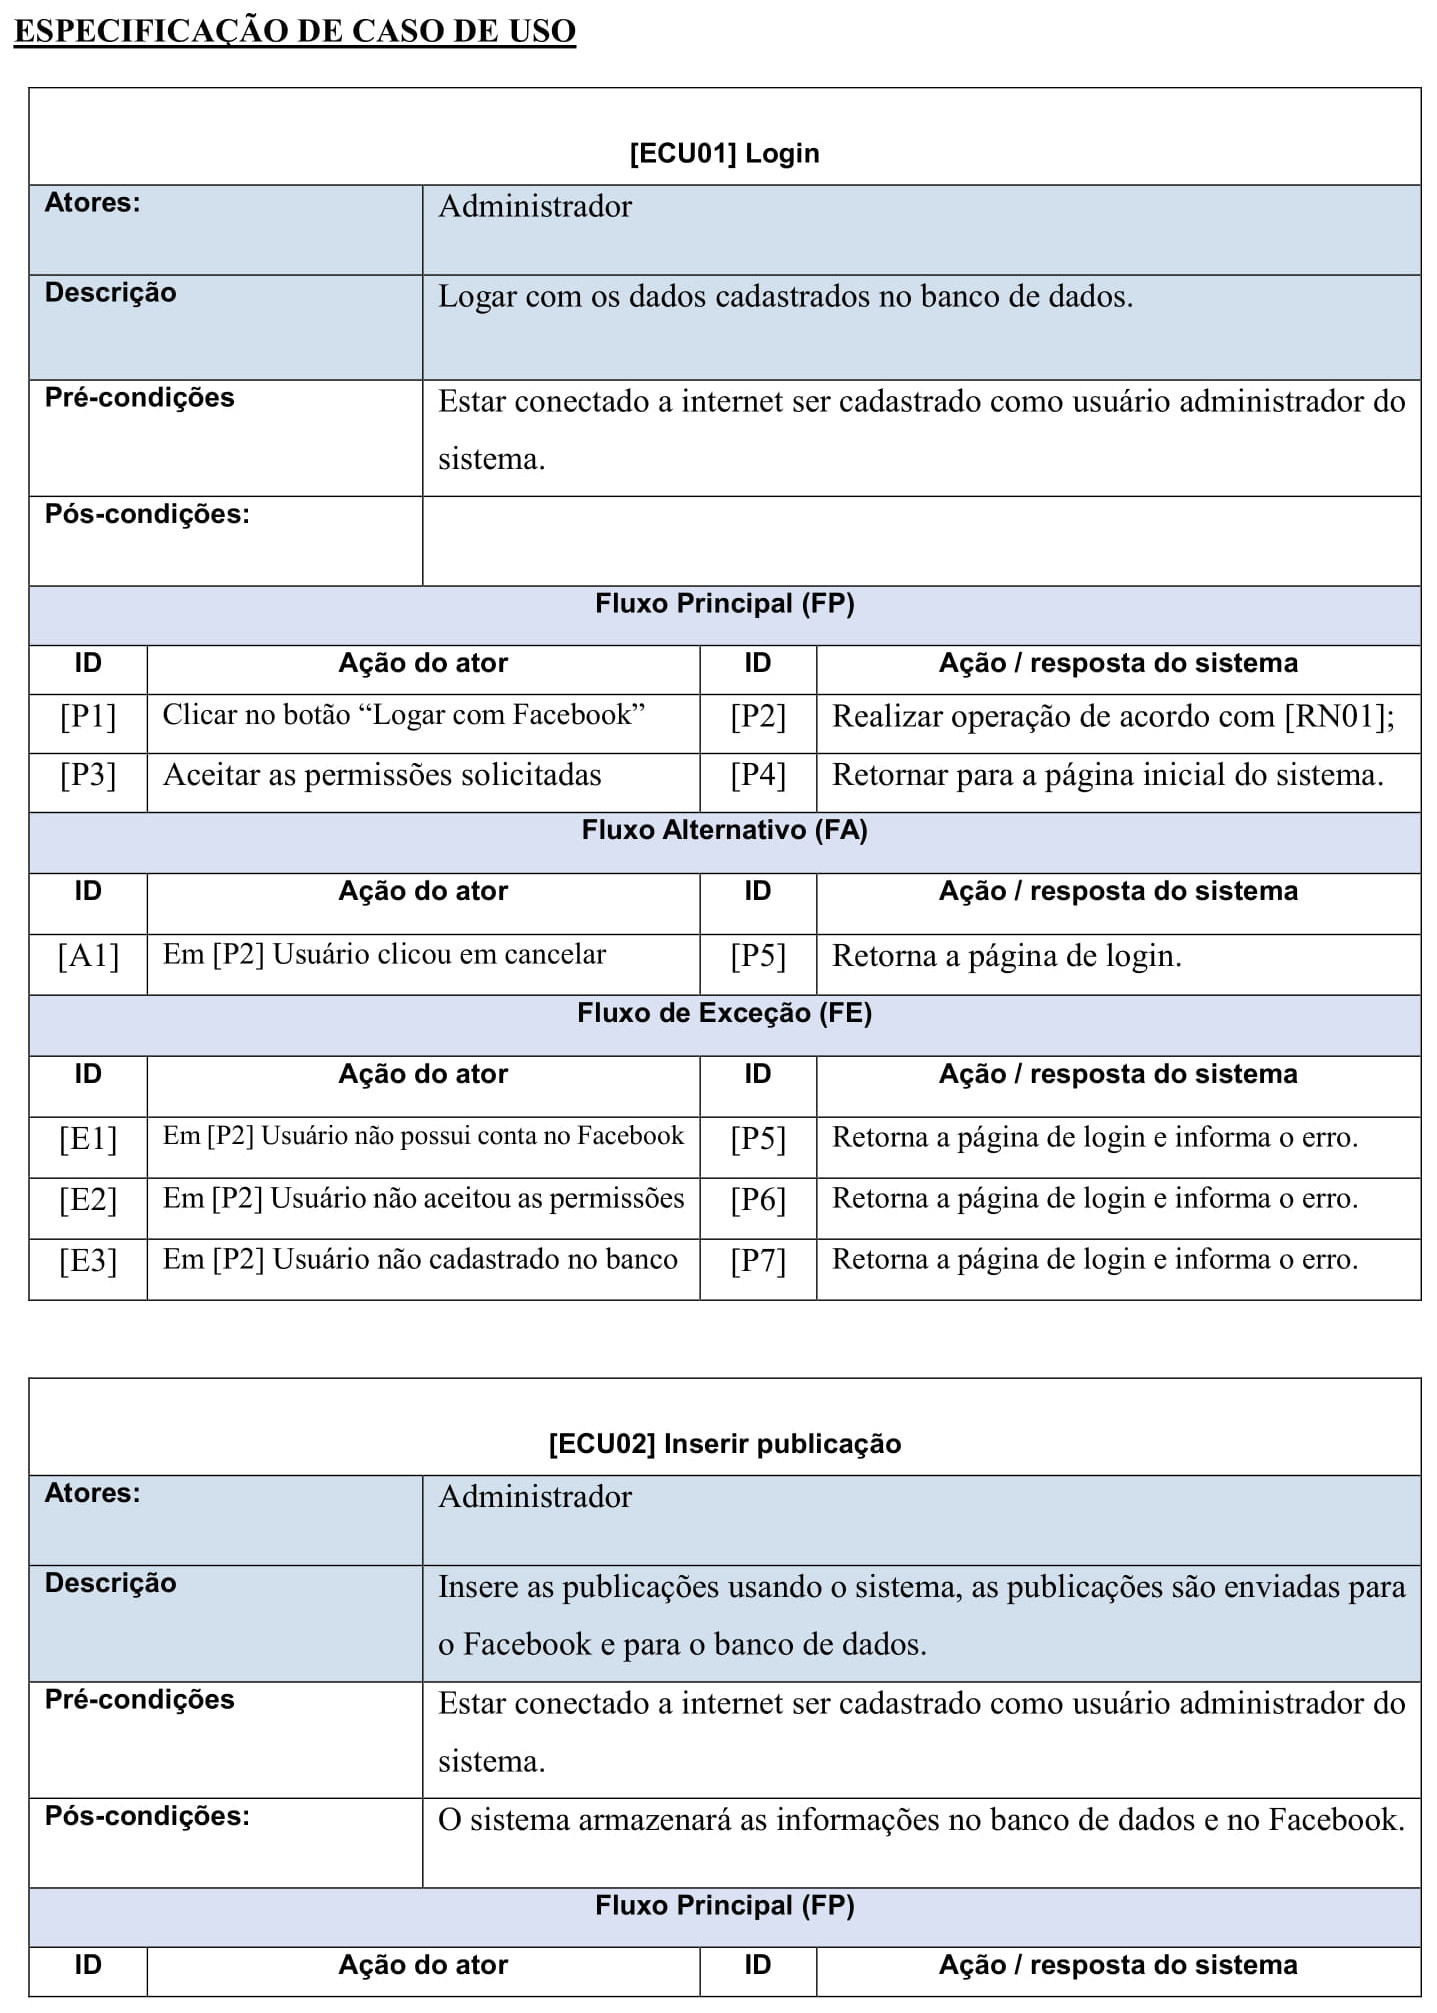
\includegraphics[width=\textwidth]{documentacao/ModeloArtefatos-06.jpg}
\end{figure}

\begin{figure}
    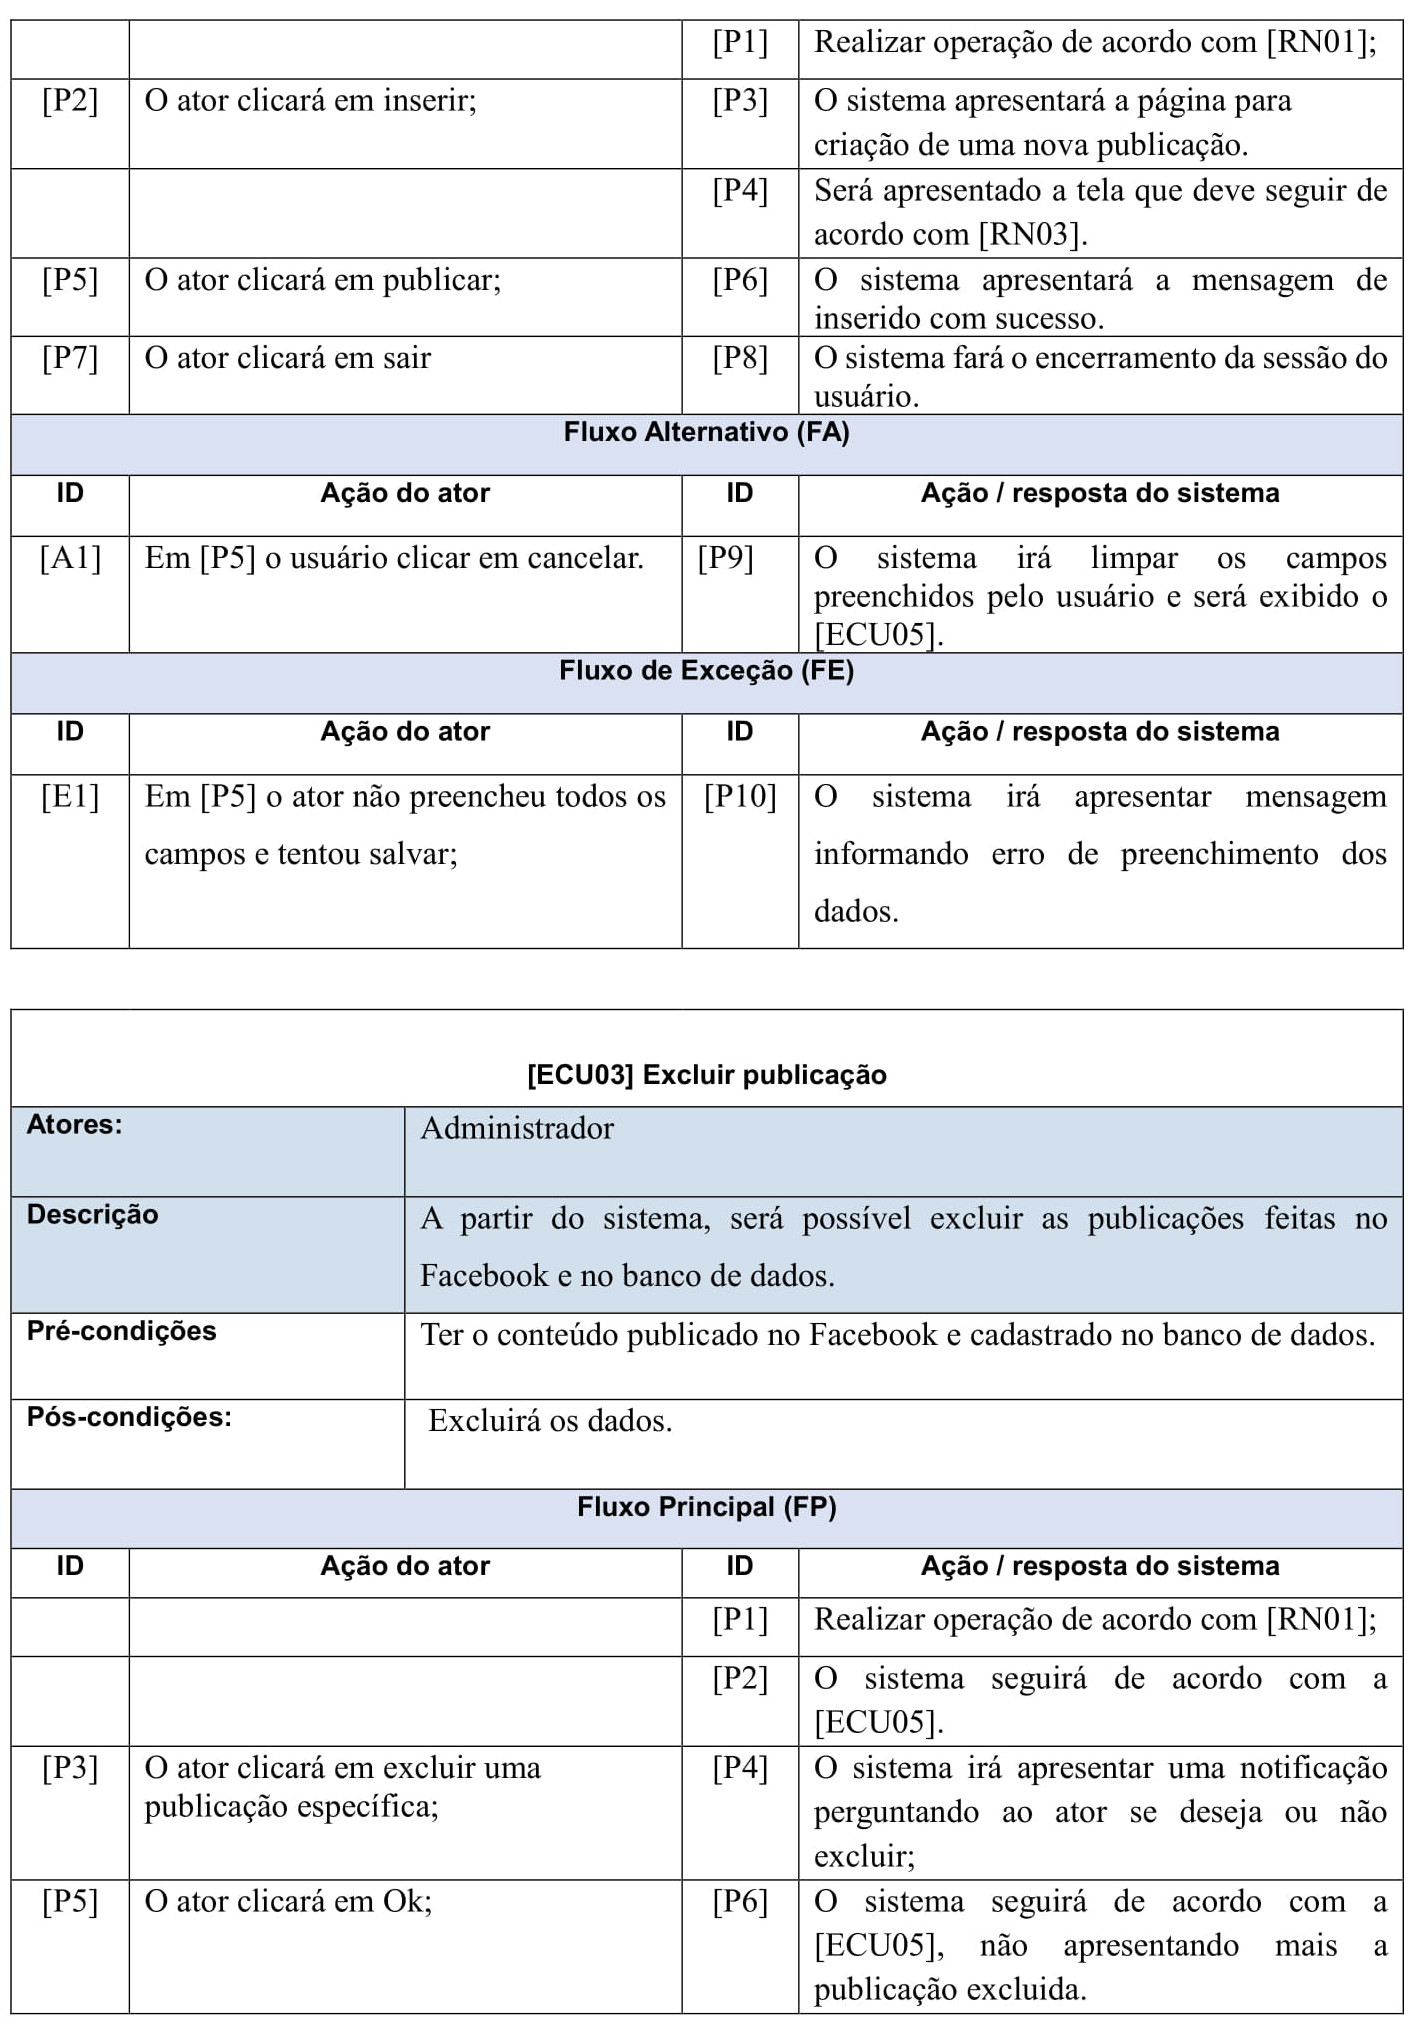
\includegraphics[width=\textwidth]{documentacao/ModeloArtefatos-07.jpg}
\end{figure}

\begin{figure}
    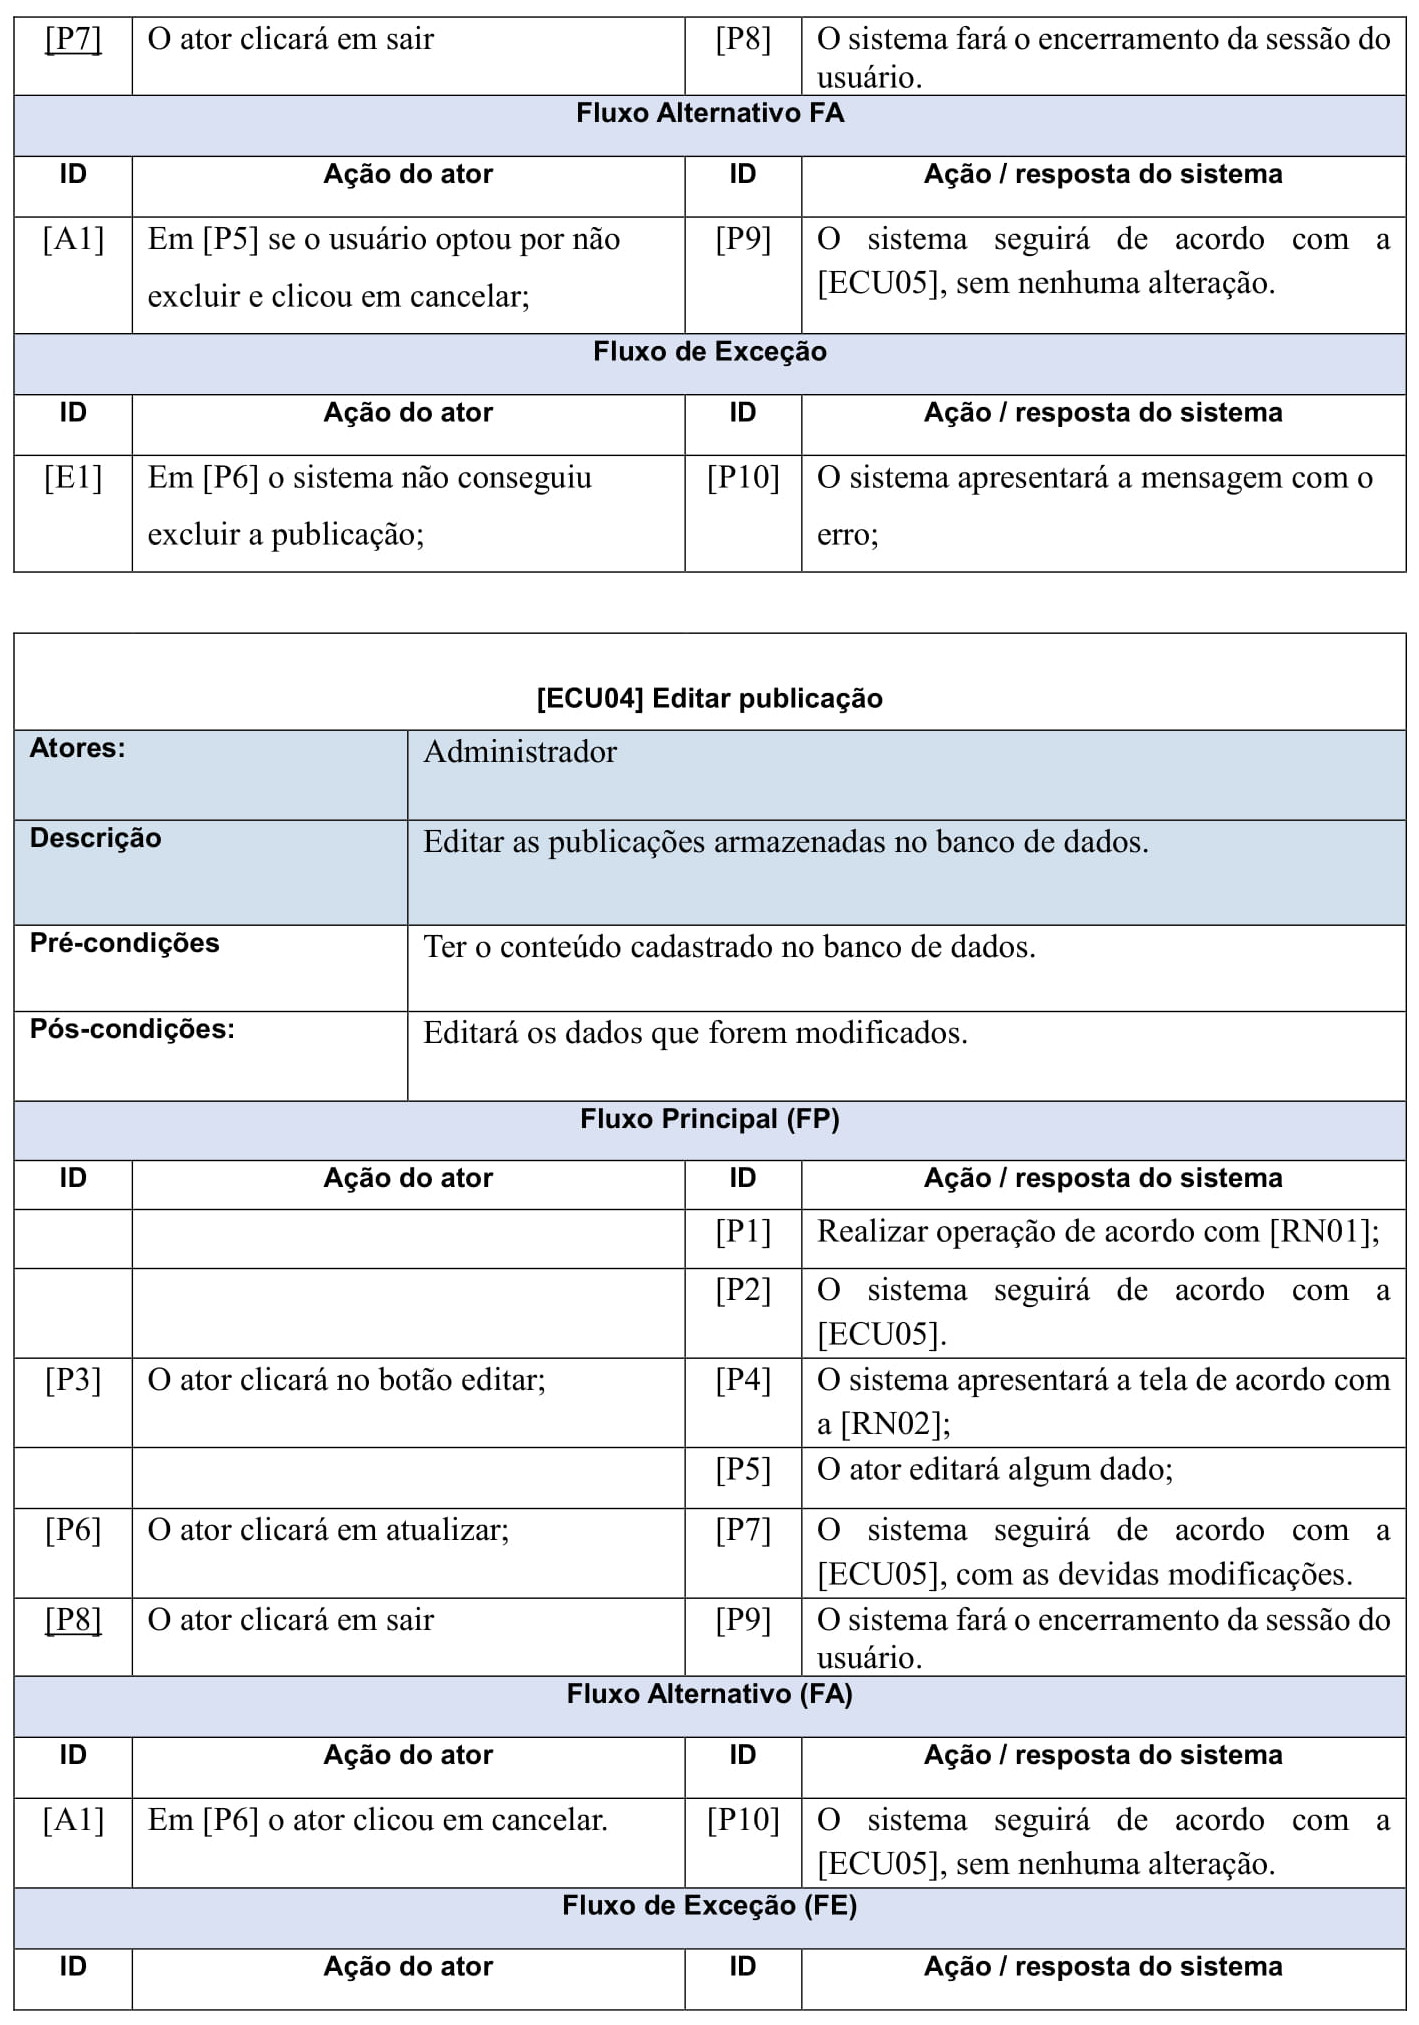
\includegraphics[width=\textwidth]{documentacao/ModeloArtefatos-08.jpg}
\end{figure}

\begin{figure}
    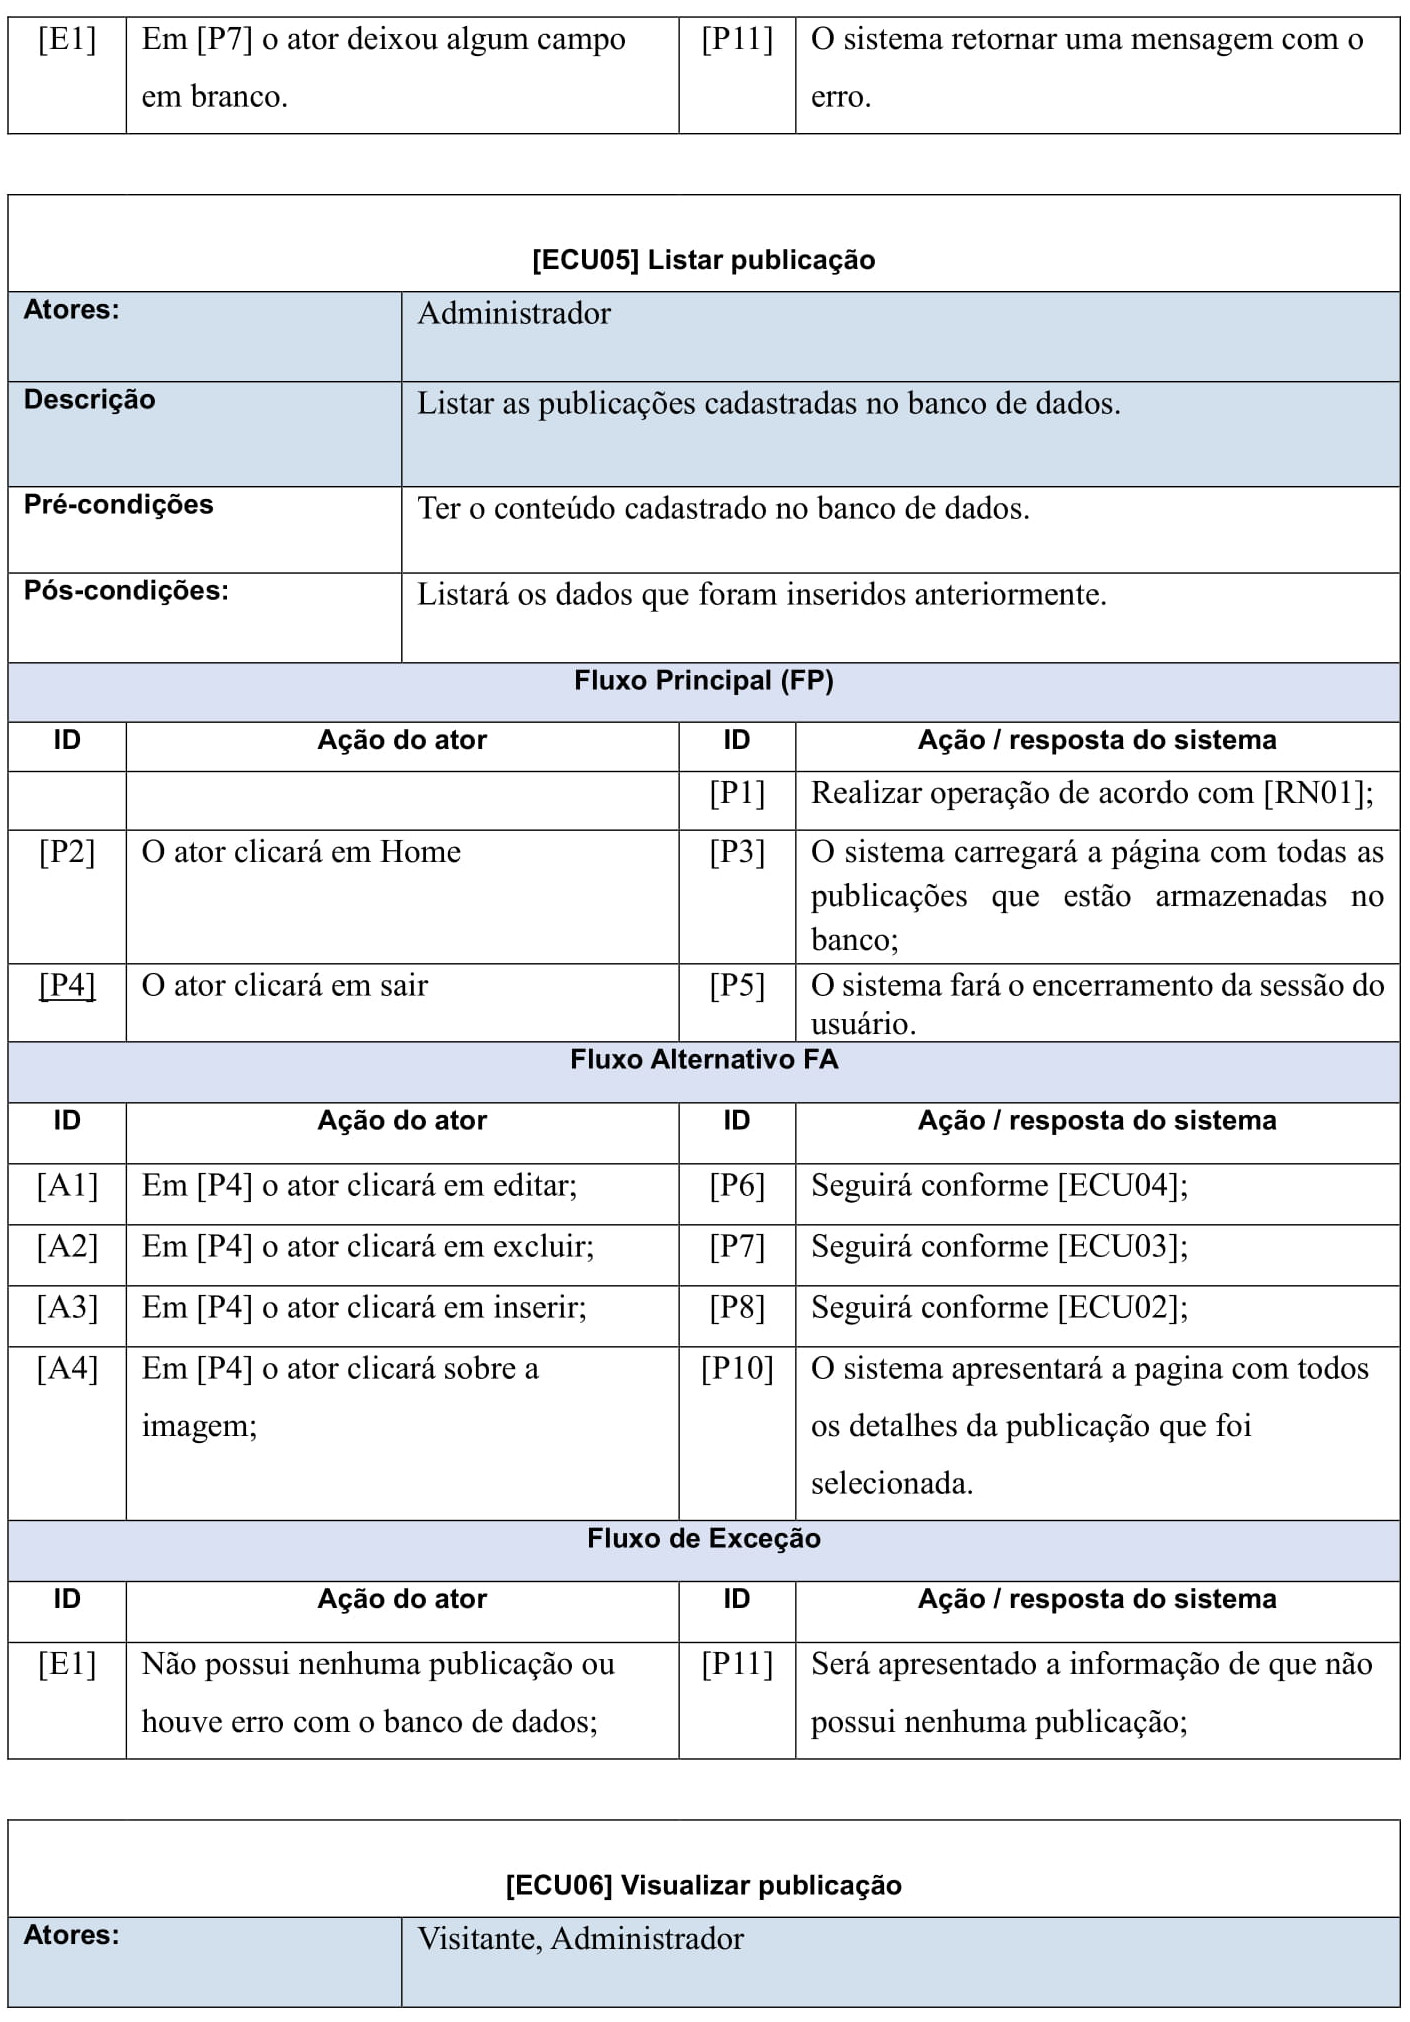
\includegraphics[width=\textwidth]{documentacao/ModeloArtefatos-09.jpg}
\end{figure}

\begin{figure}[H]
    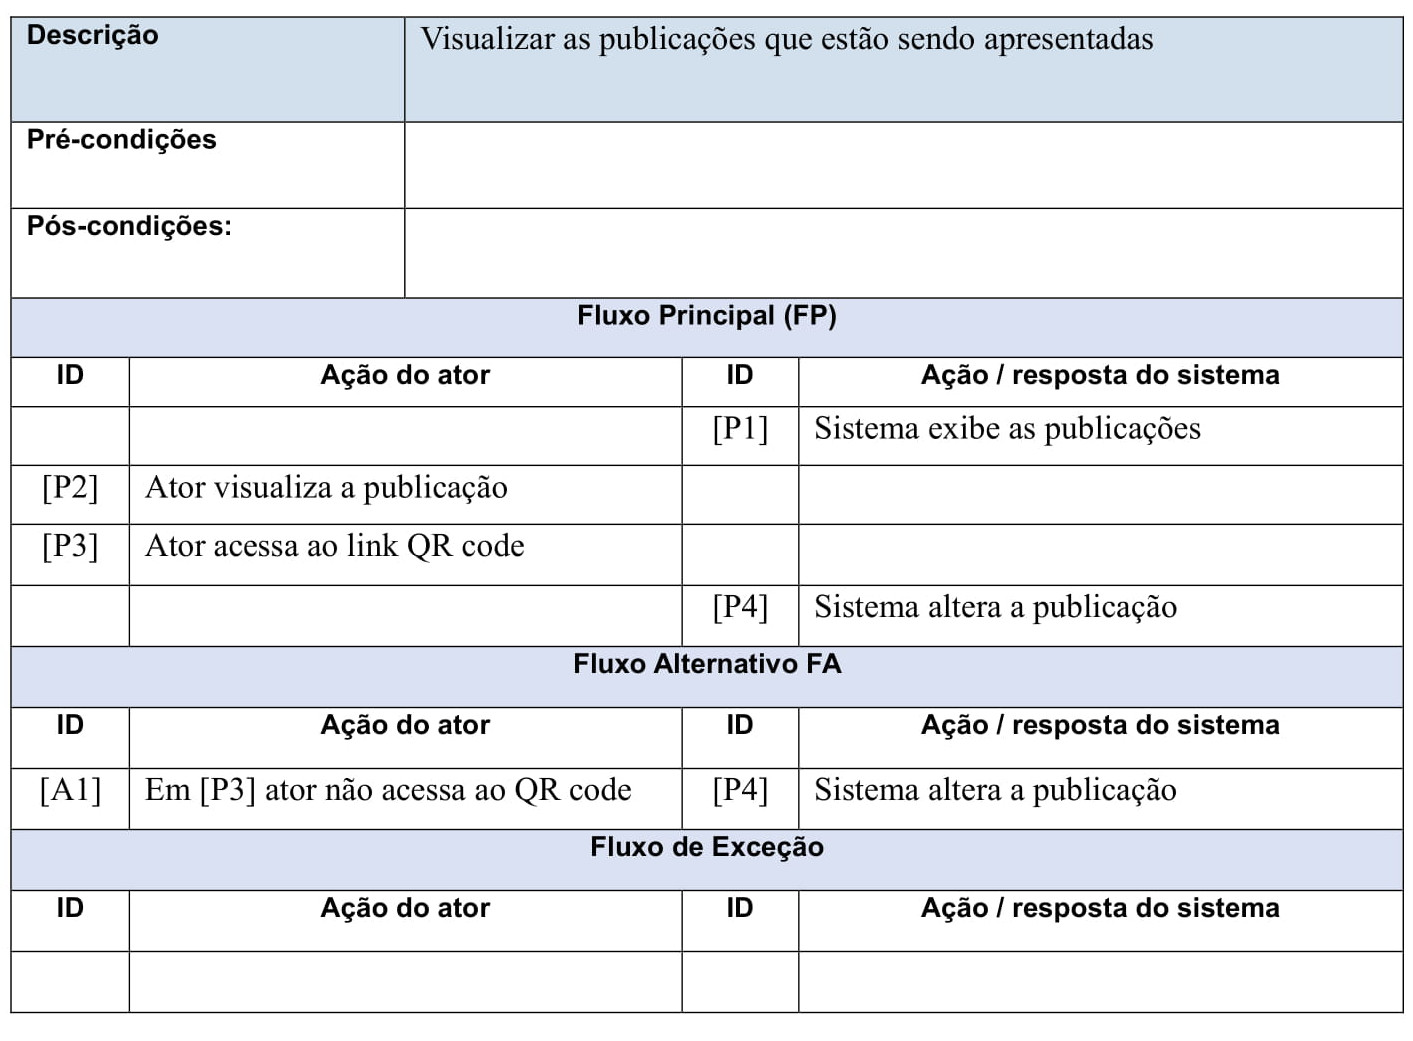
\includegraphics[width=\textwidth]{documentacao/ModeloArtefatos-10.jpg}
\end{figure}



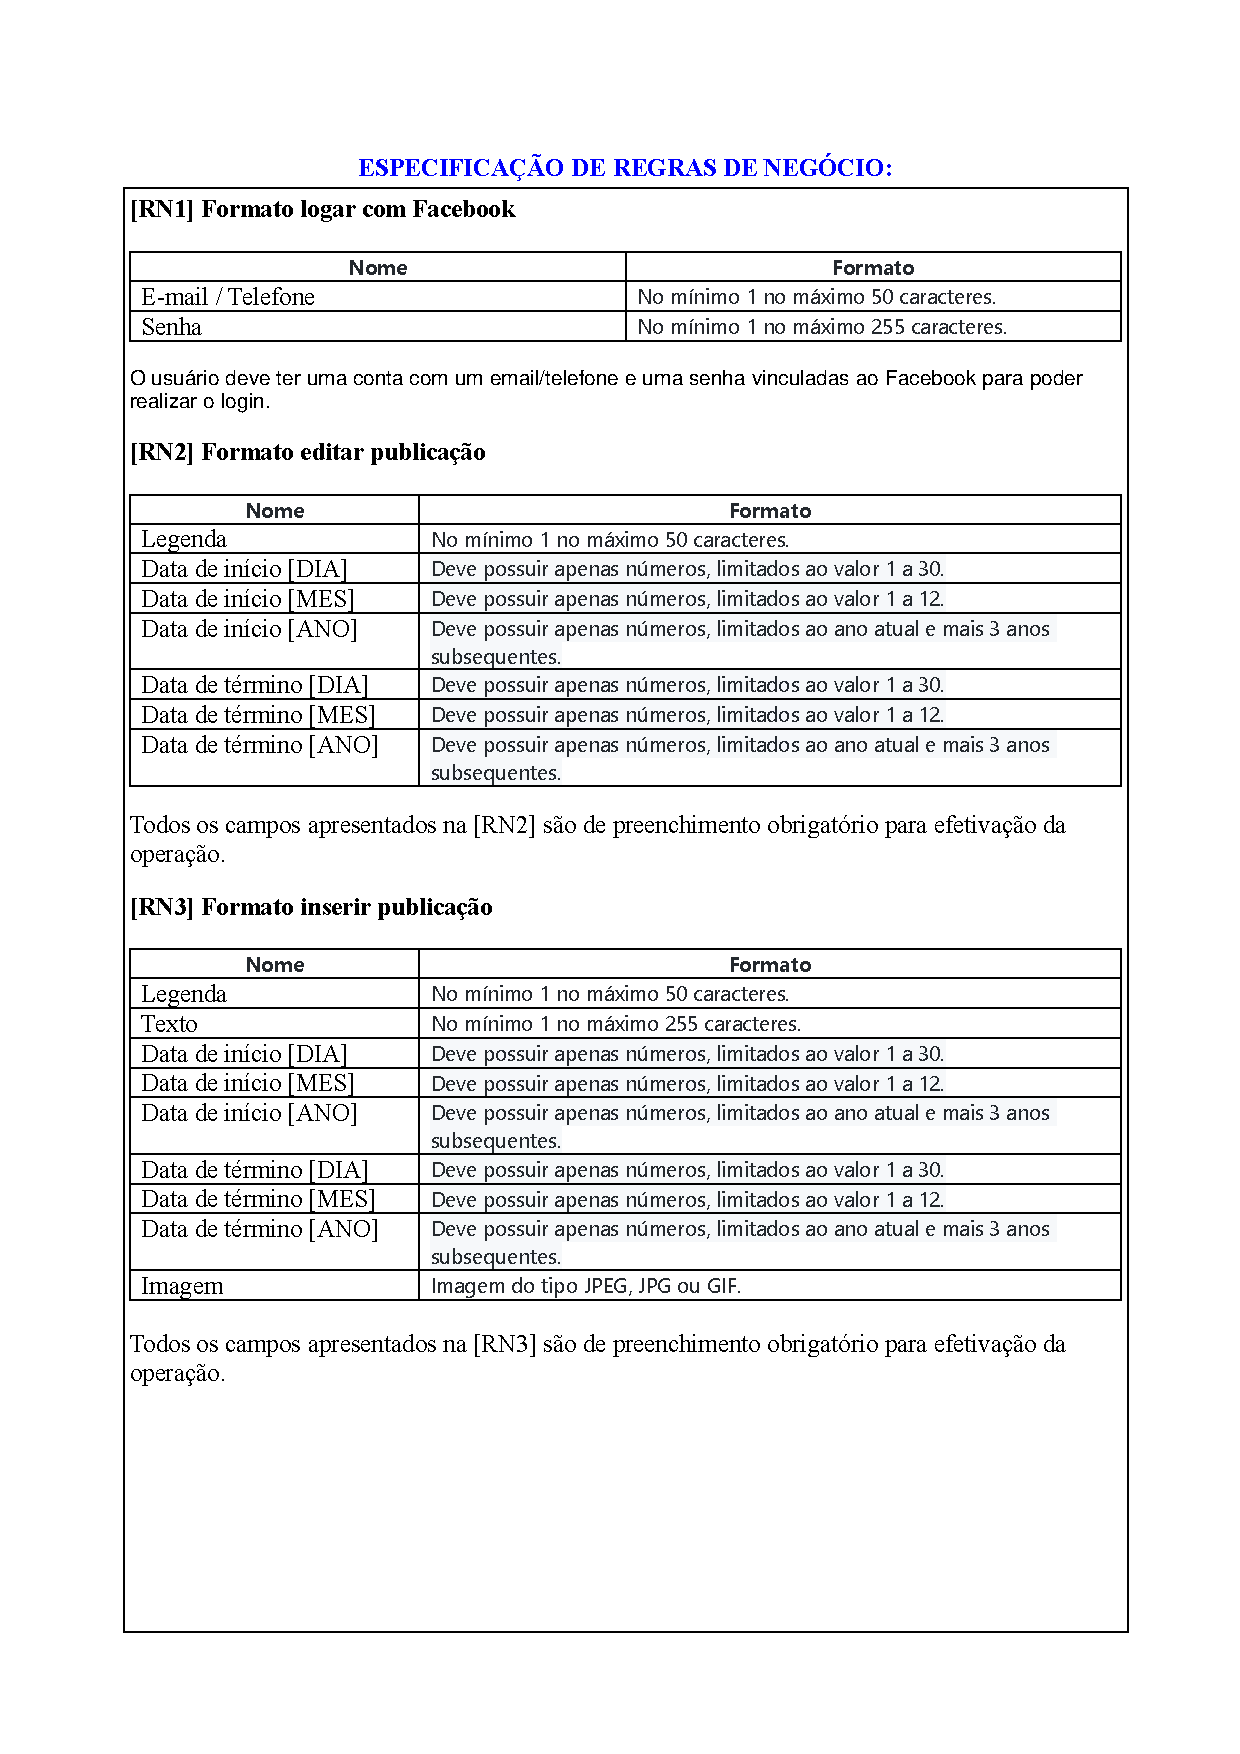
\includepdf[pages=-]{documentacao/ModeloArtefatos.pdf}

\end{document}
